\documentclass[../main.tex]{subfiles}
\begin{document}
		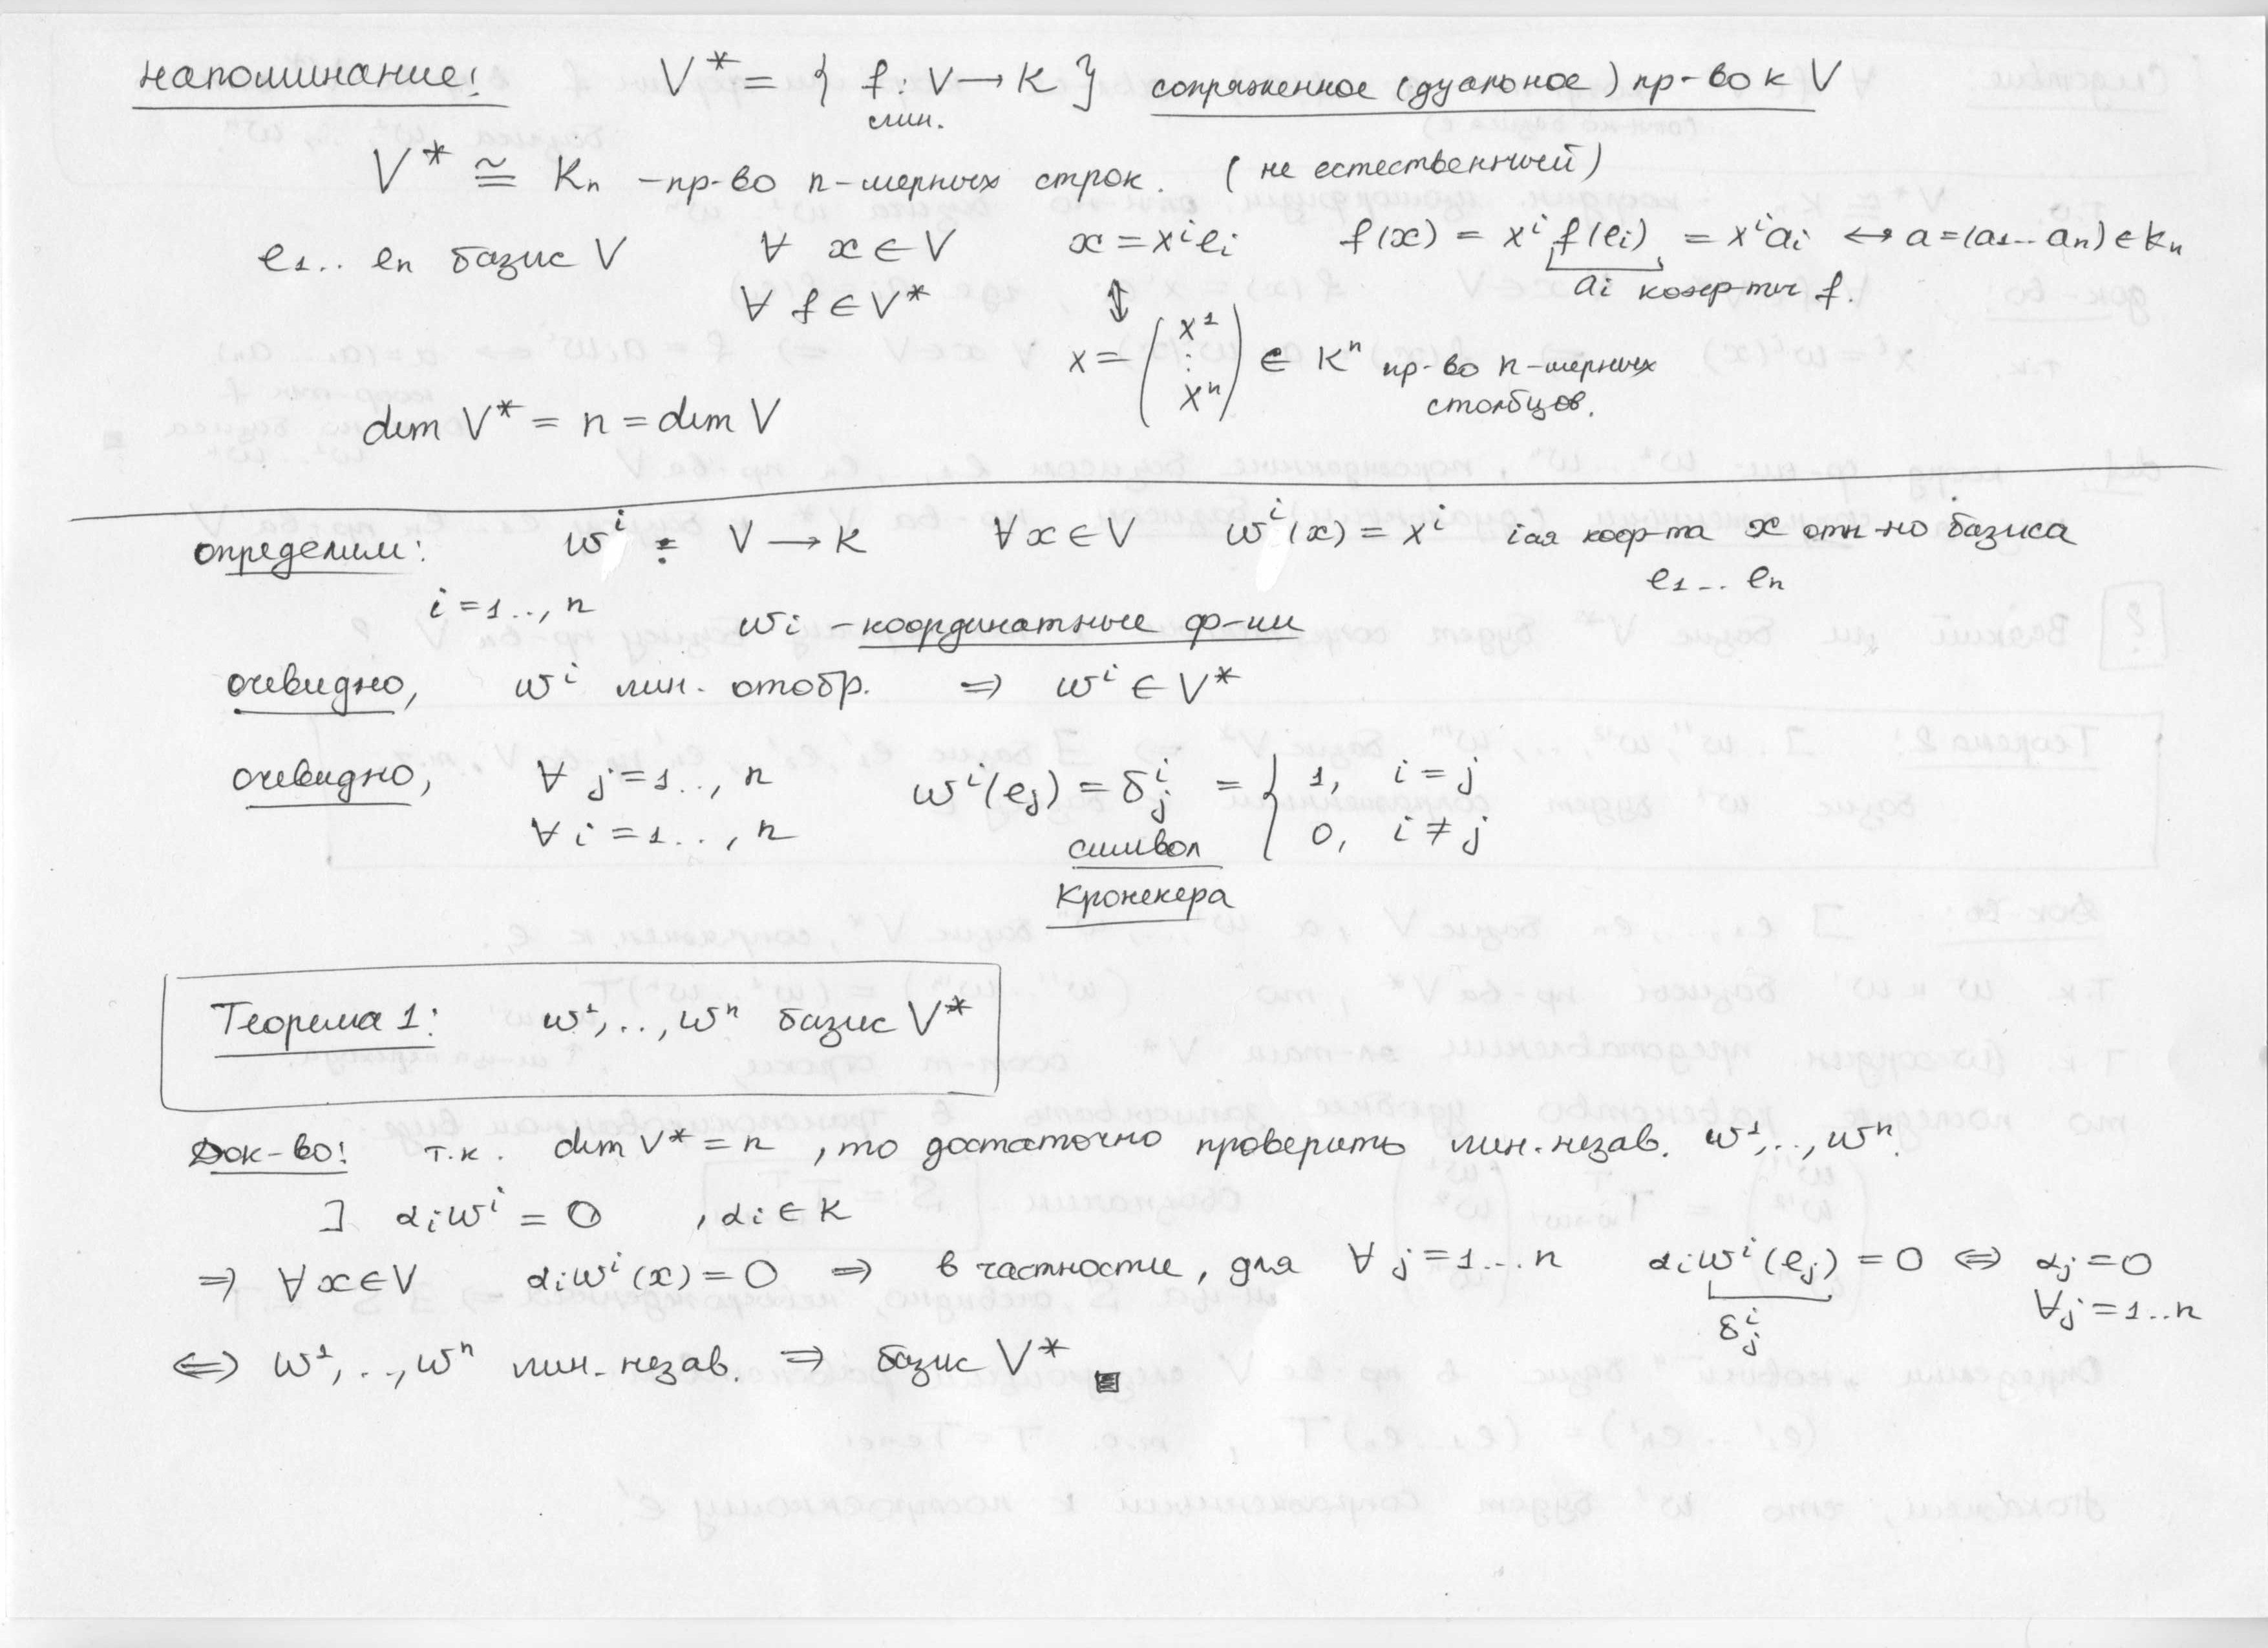
\includegraphics[height=0.49\textheight, width=\textwidth]{8_1-1}	
		\n
		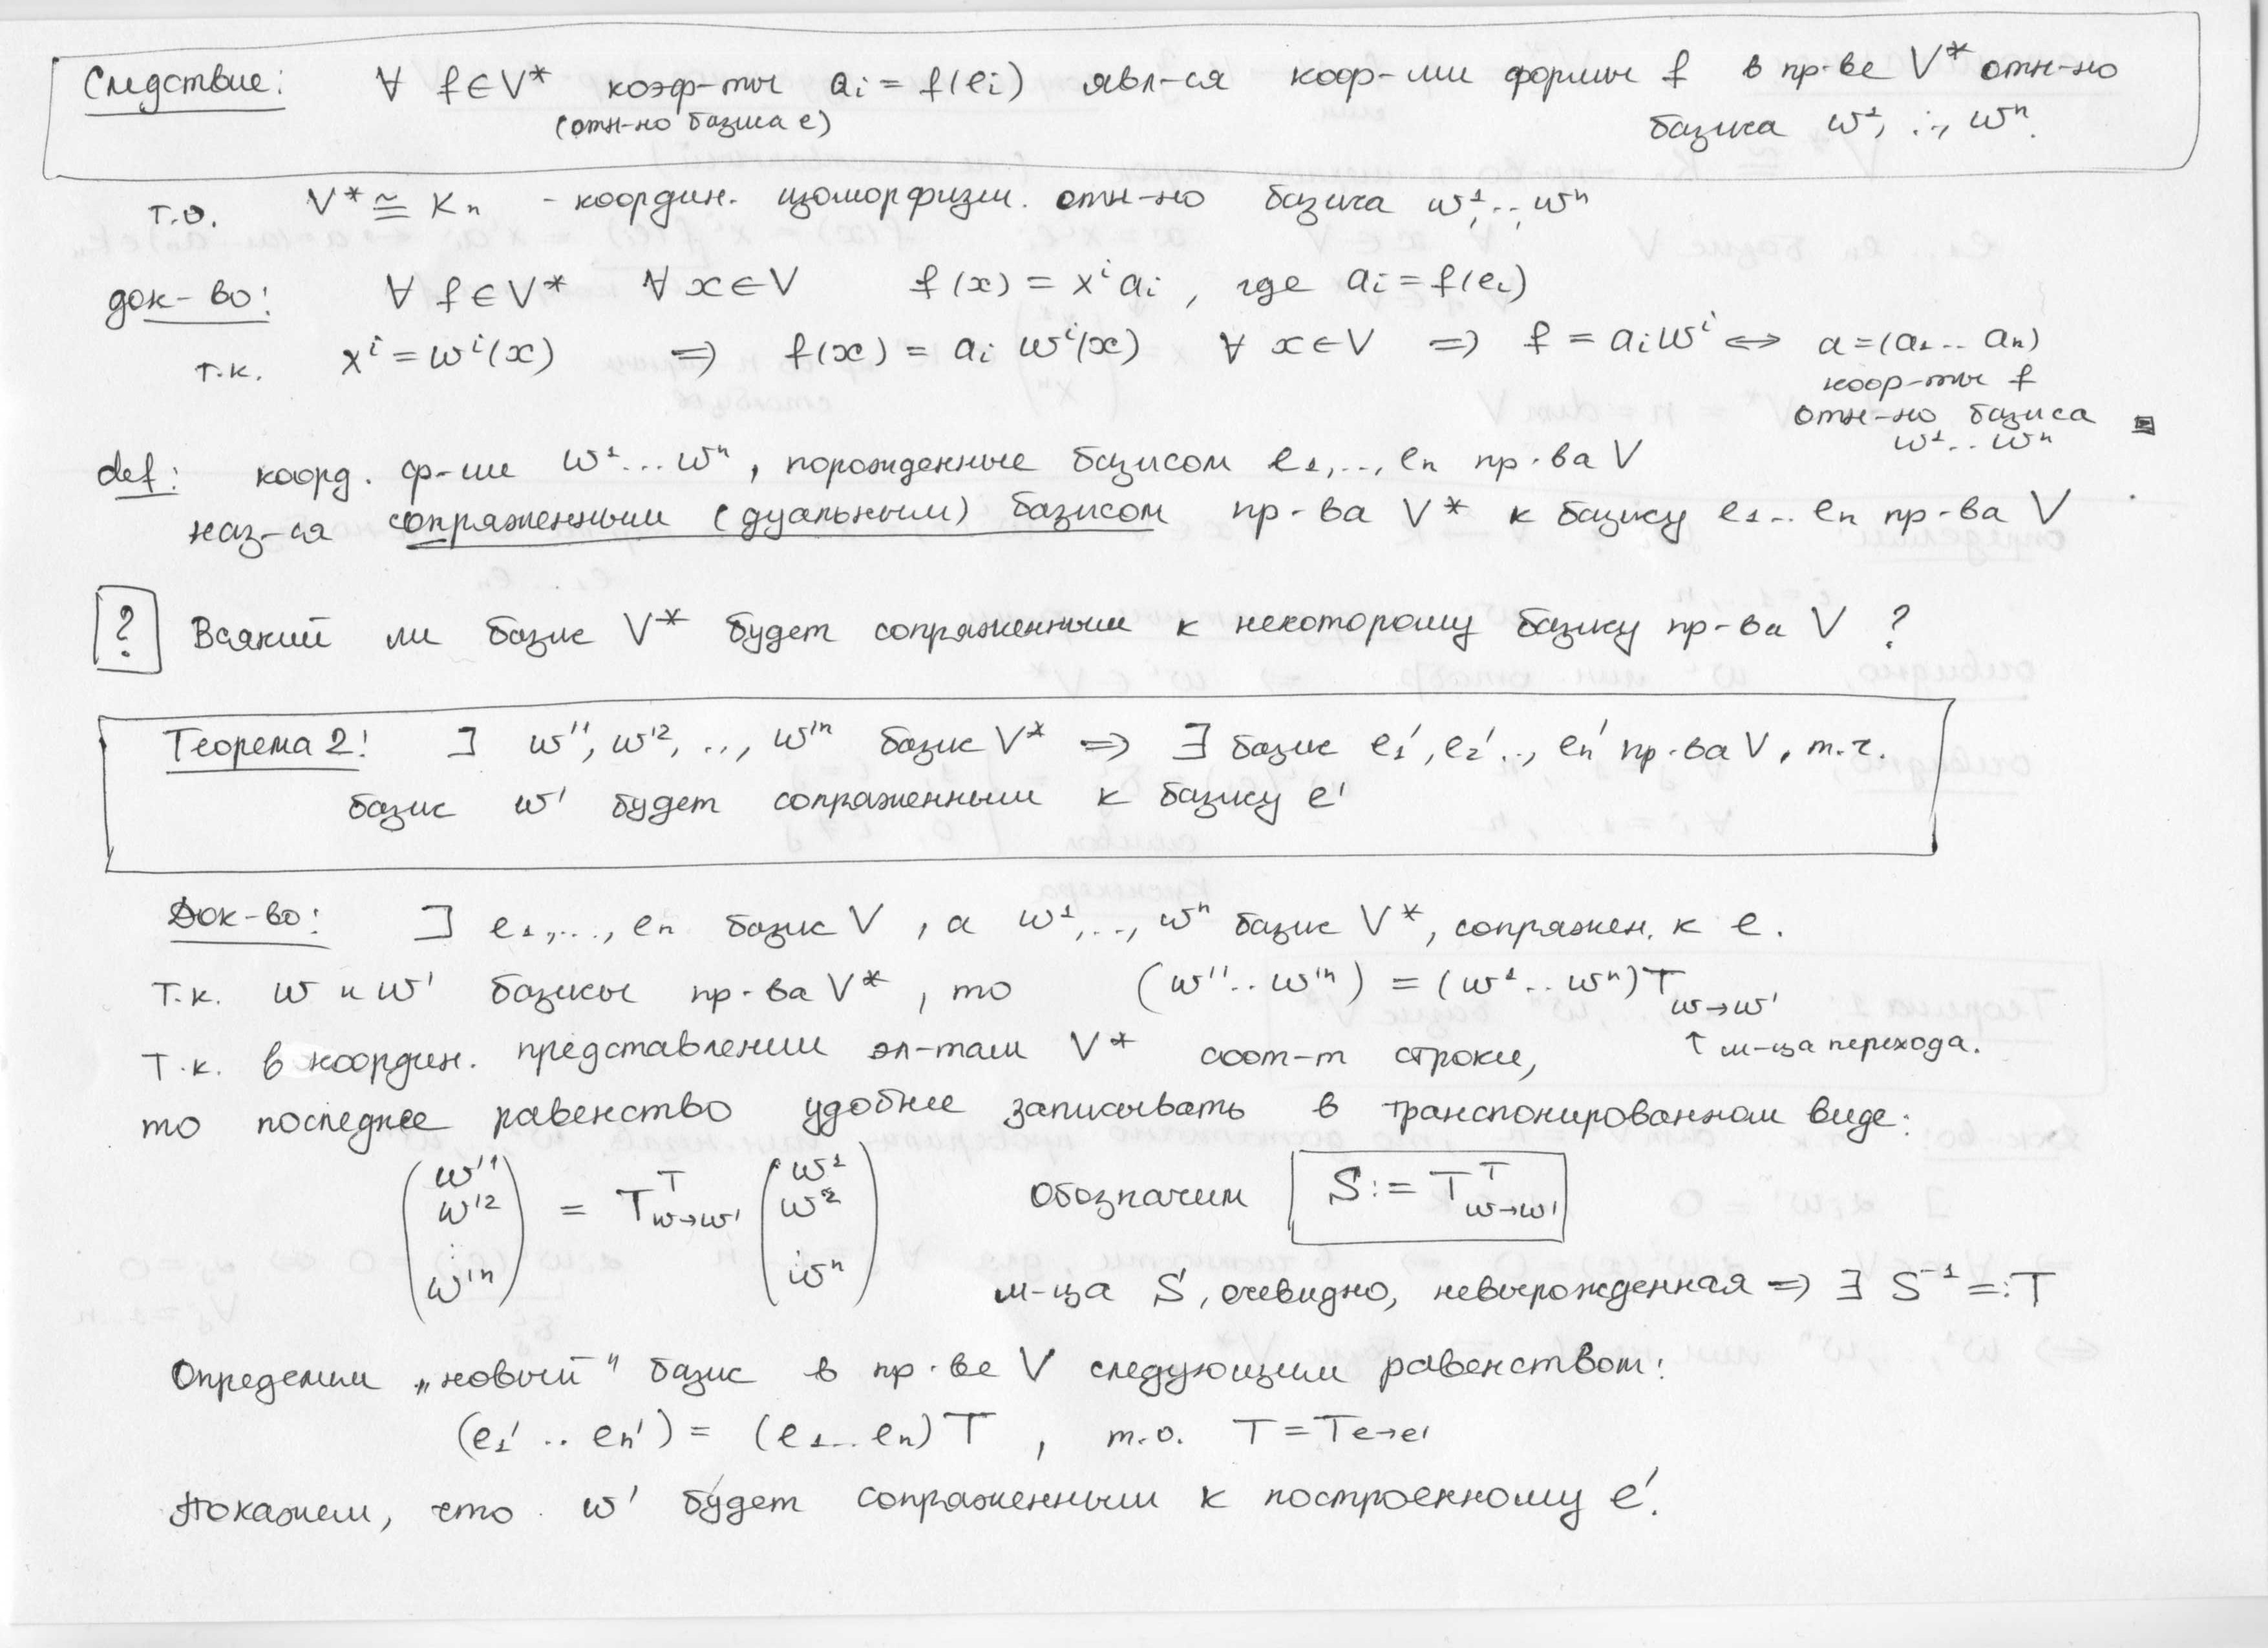
\includegraphics[height=0.49\textheight, width=\textwidth]{8_1-2}	
		\n
		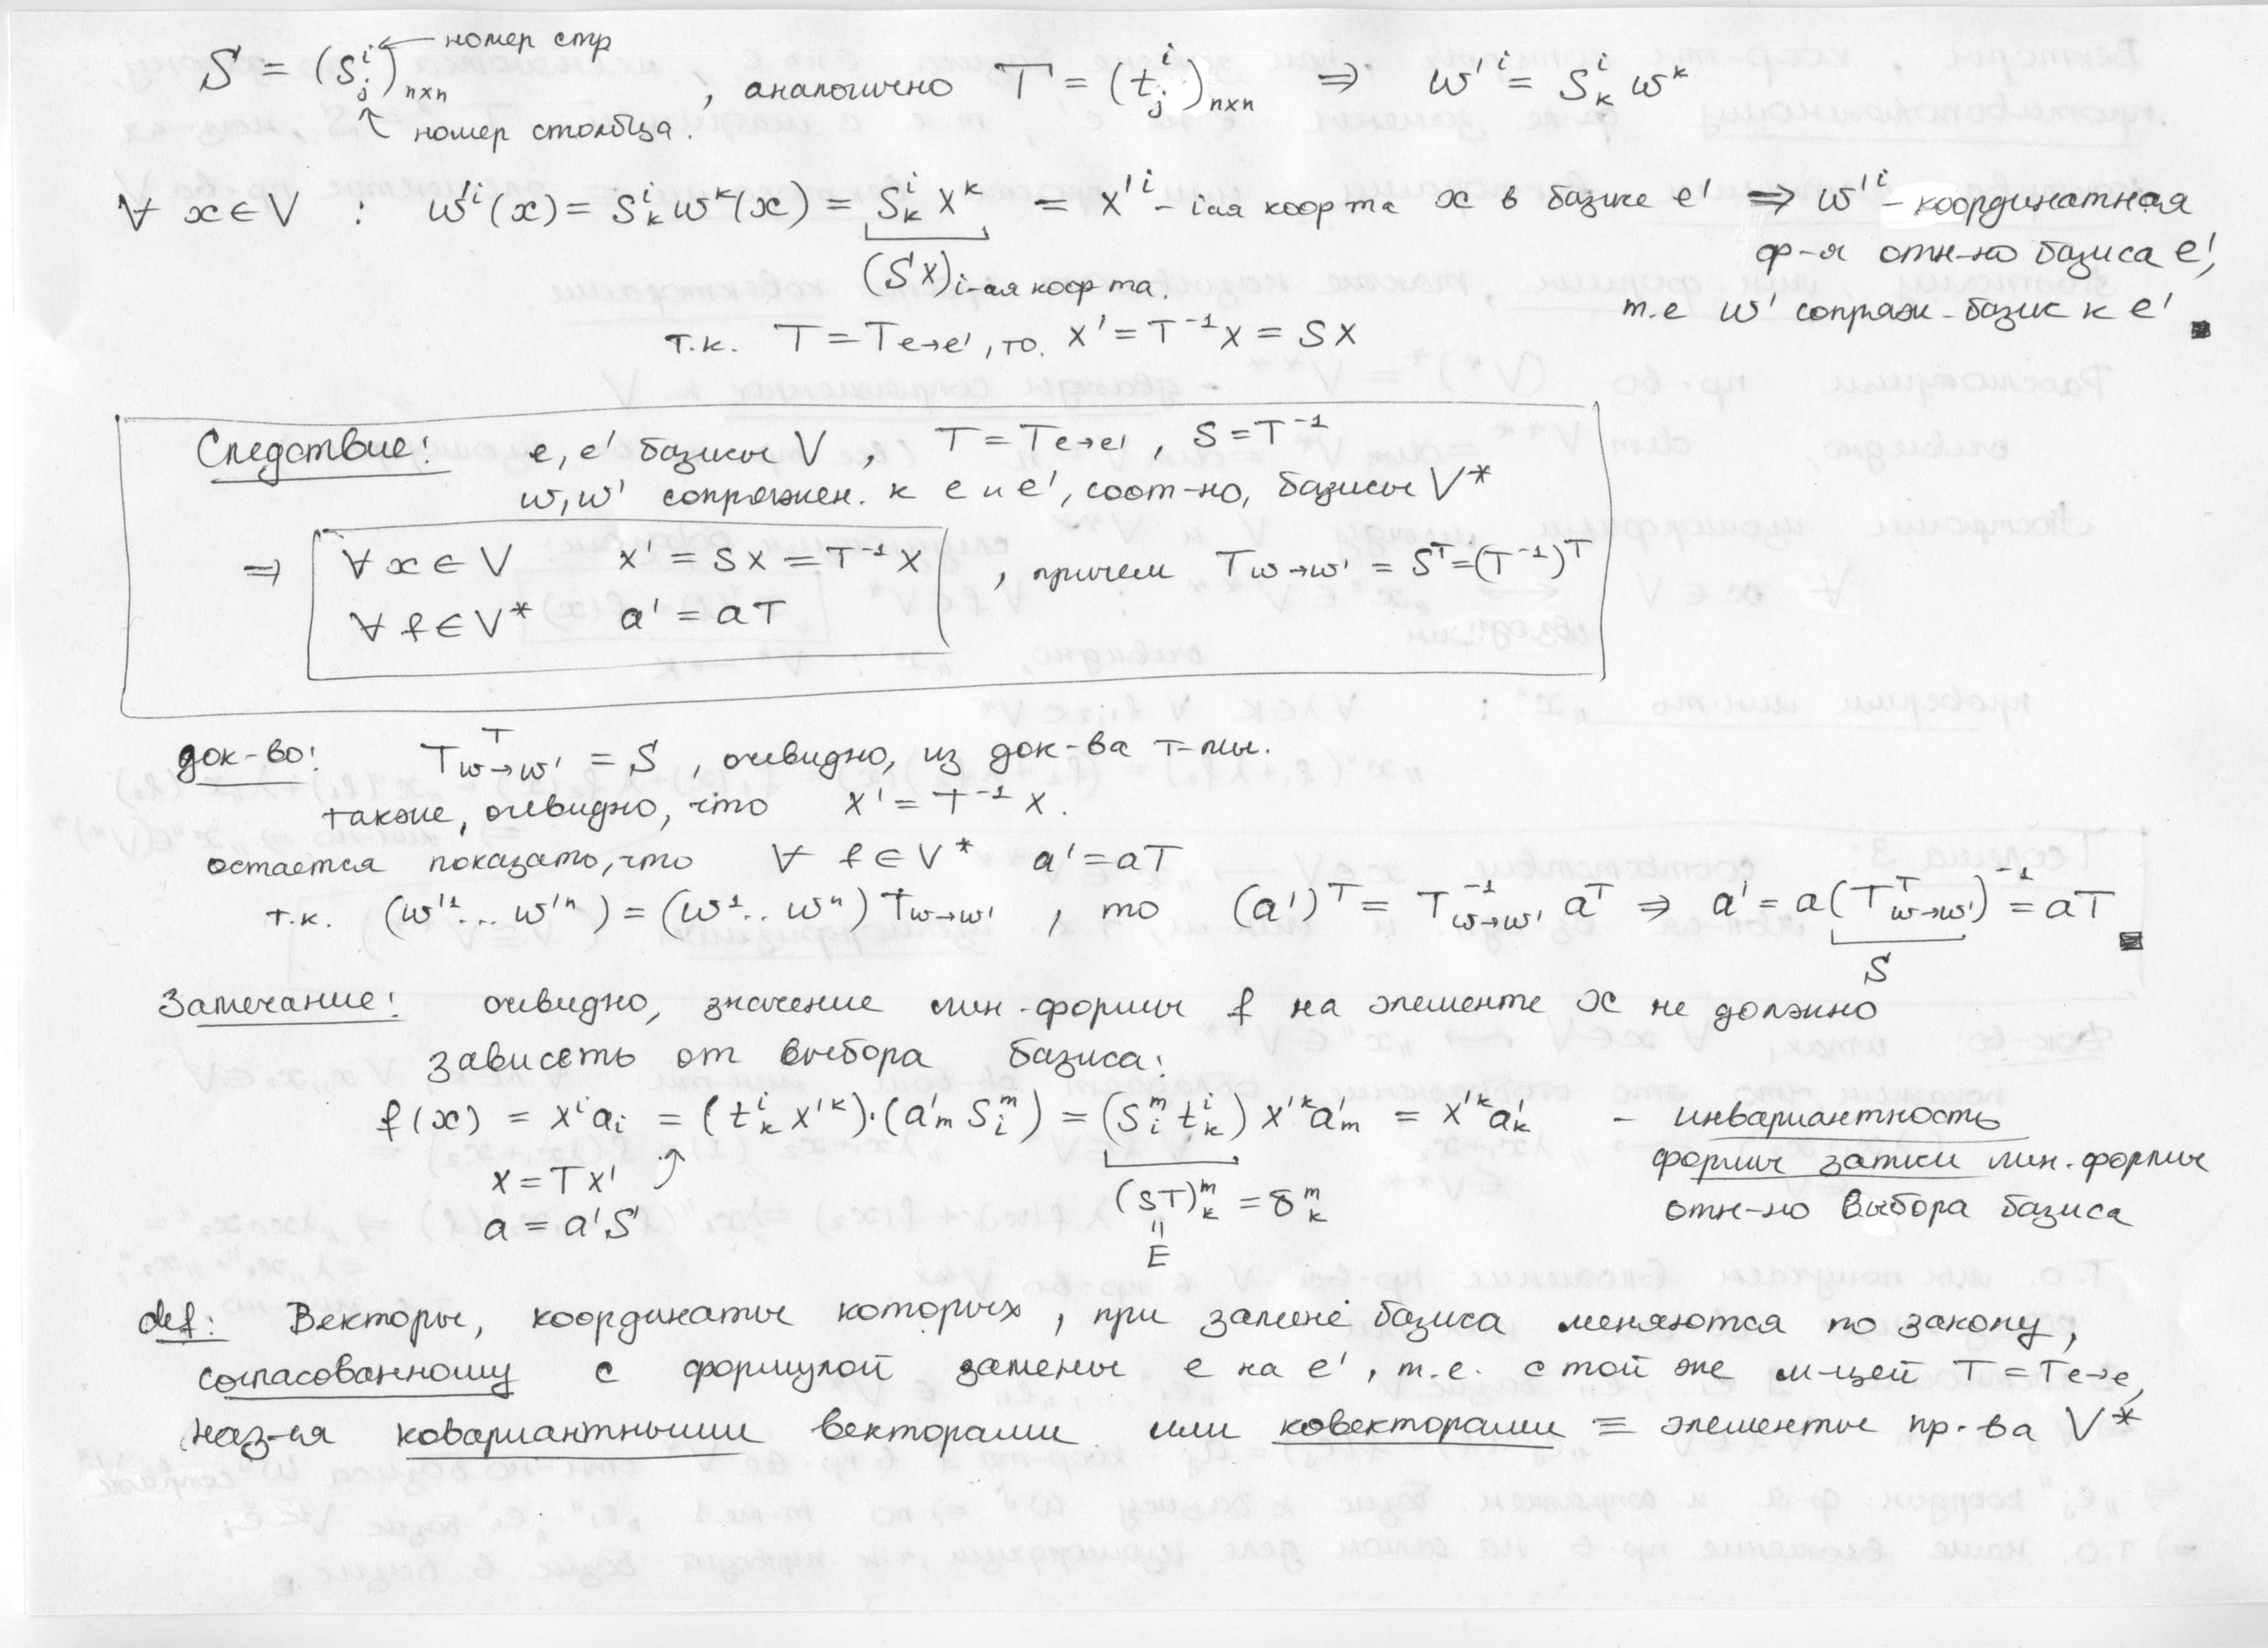
\includegraphics[height=0.49\textheight, width=\textwidth]{8_1-3}	
		\n
		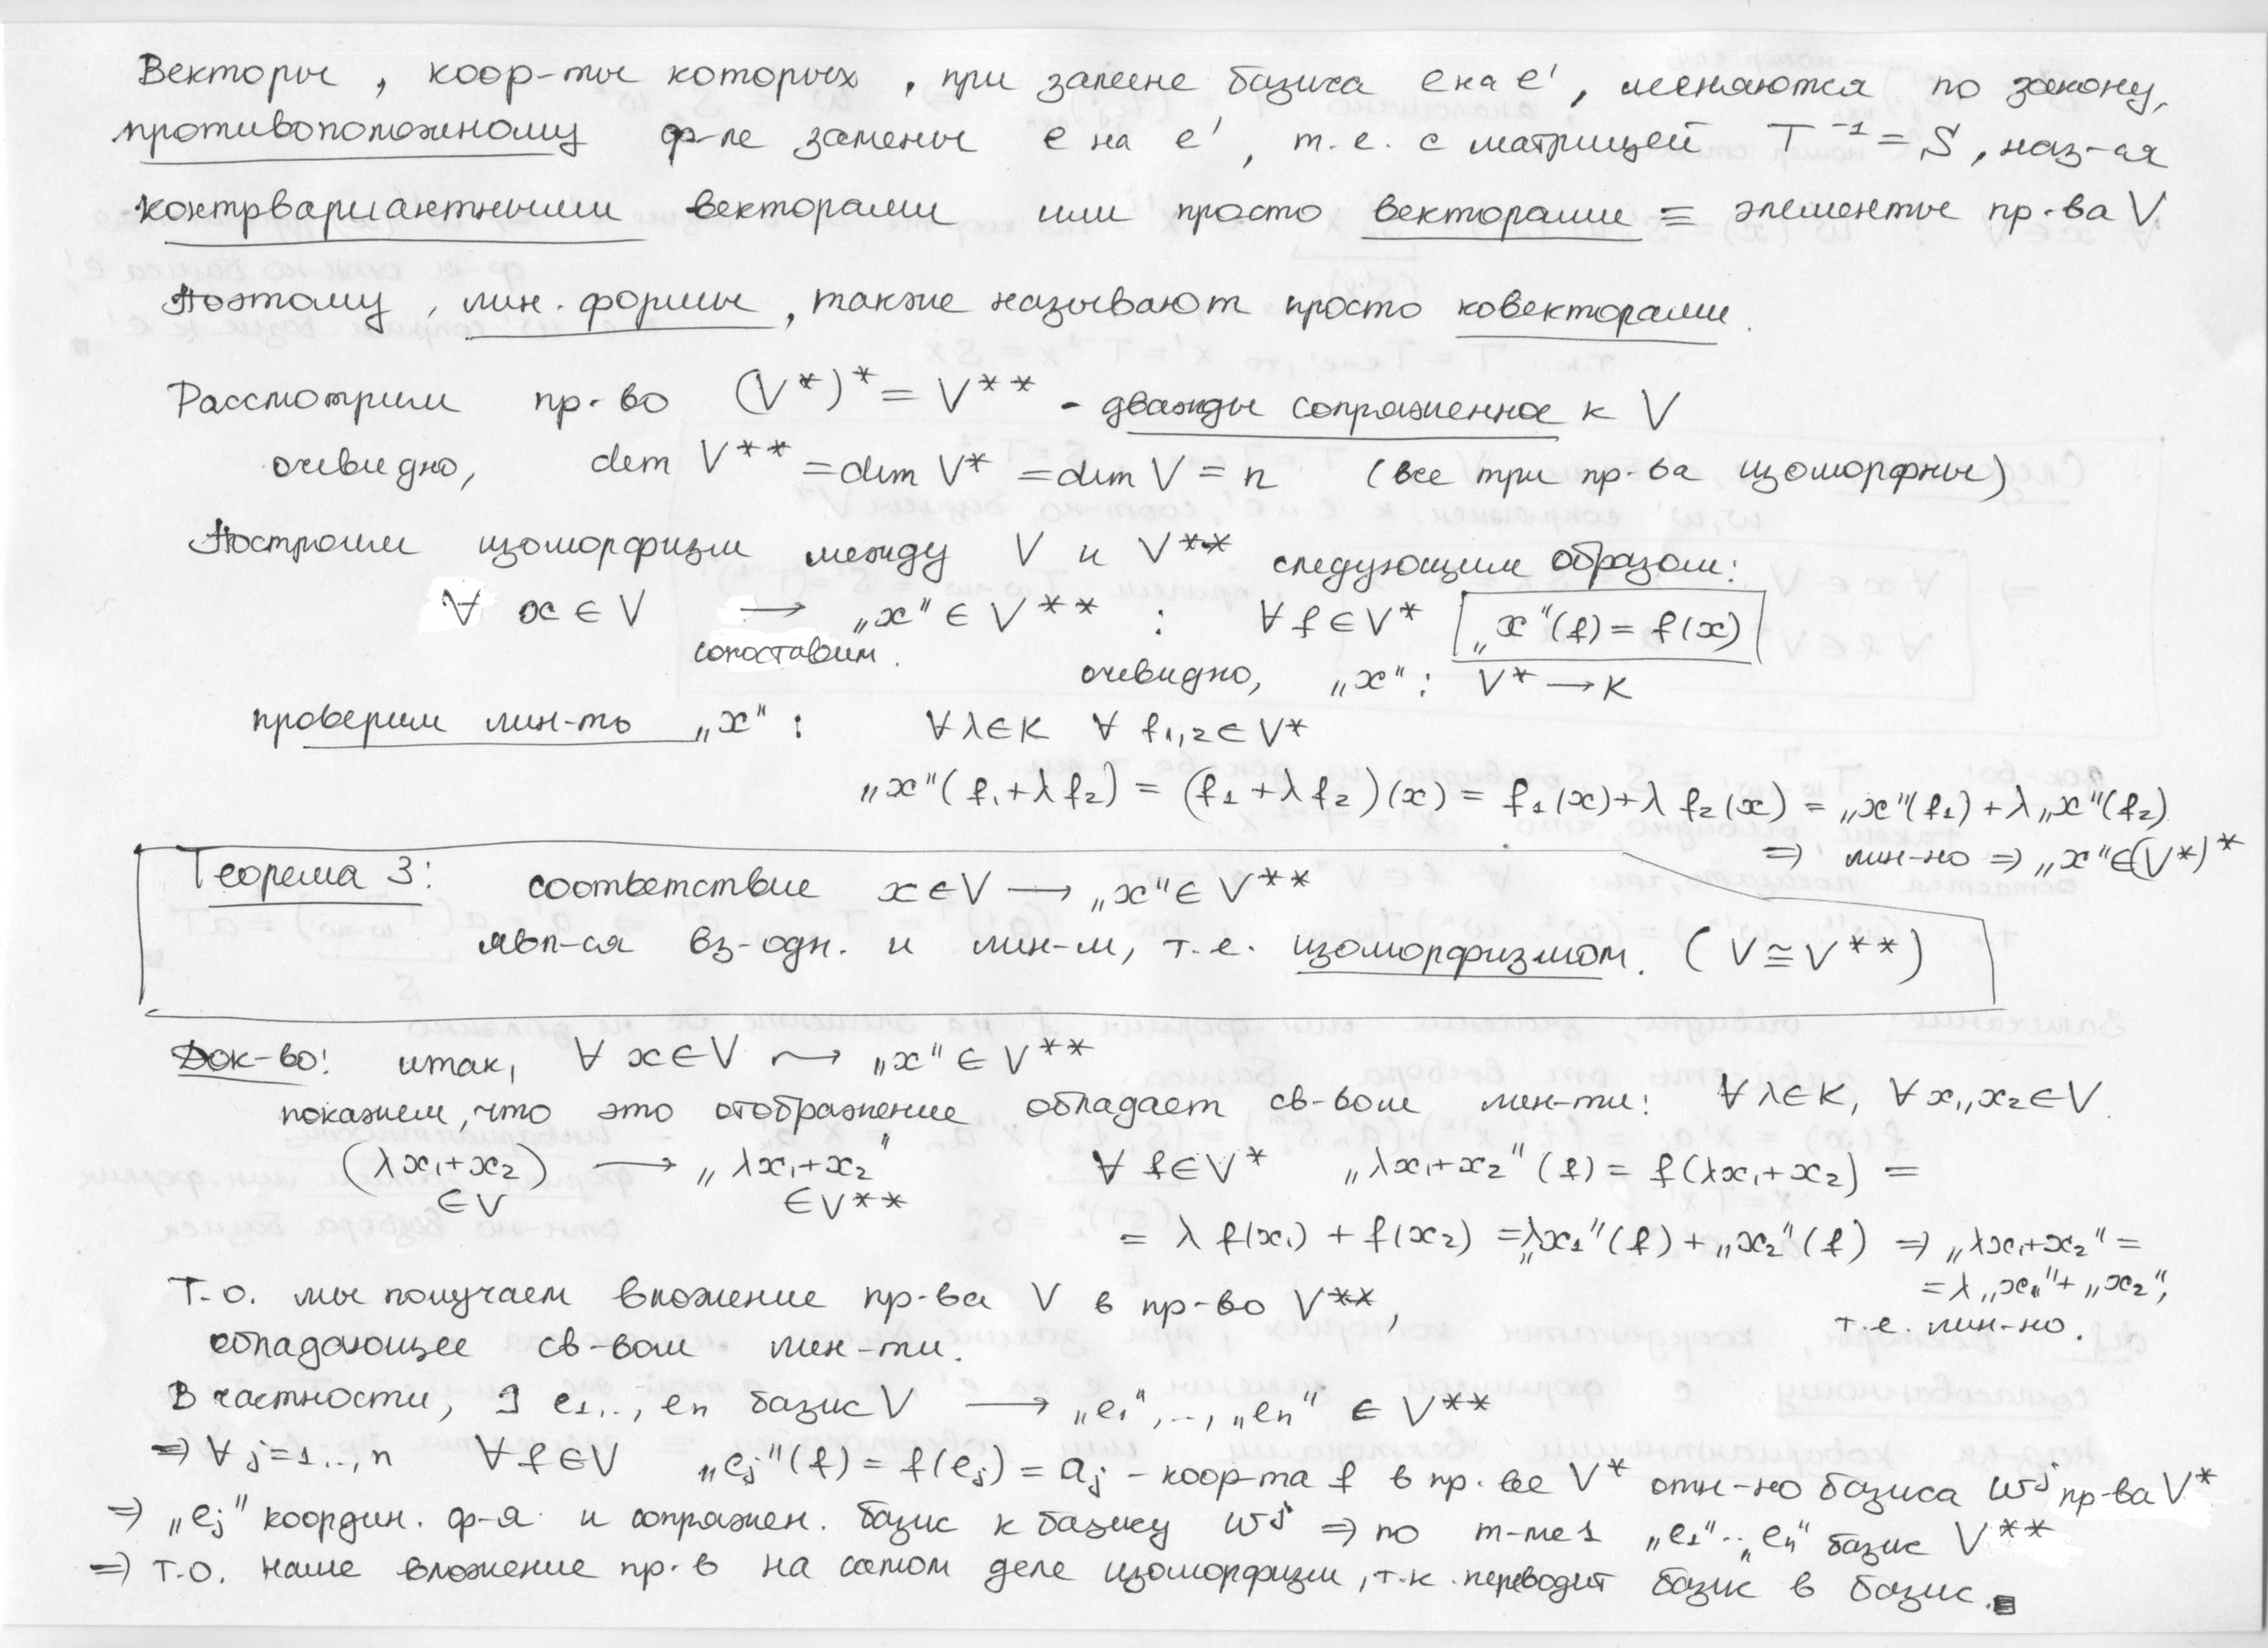
\includegraphics[height=0.49\textheight, width=\textwidth]{8_1-4}	
		\n
		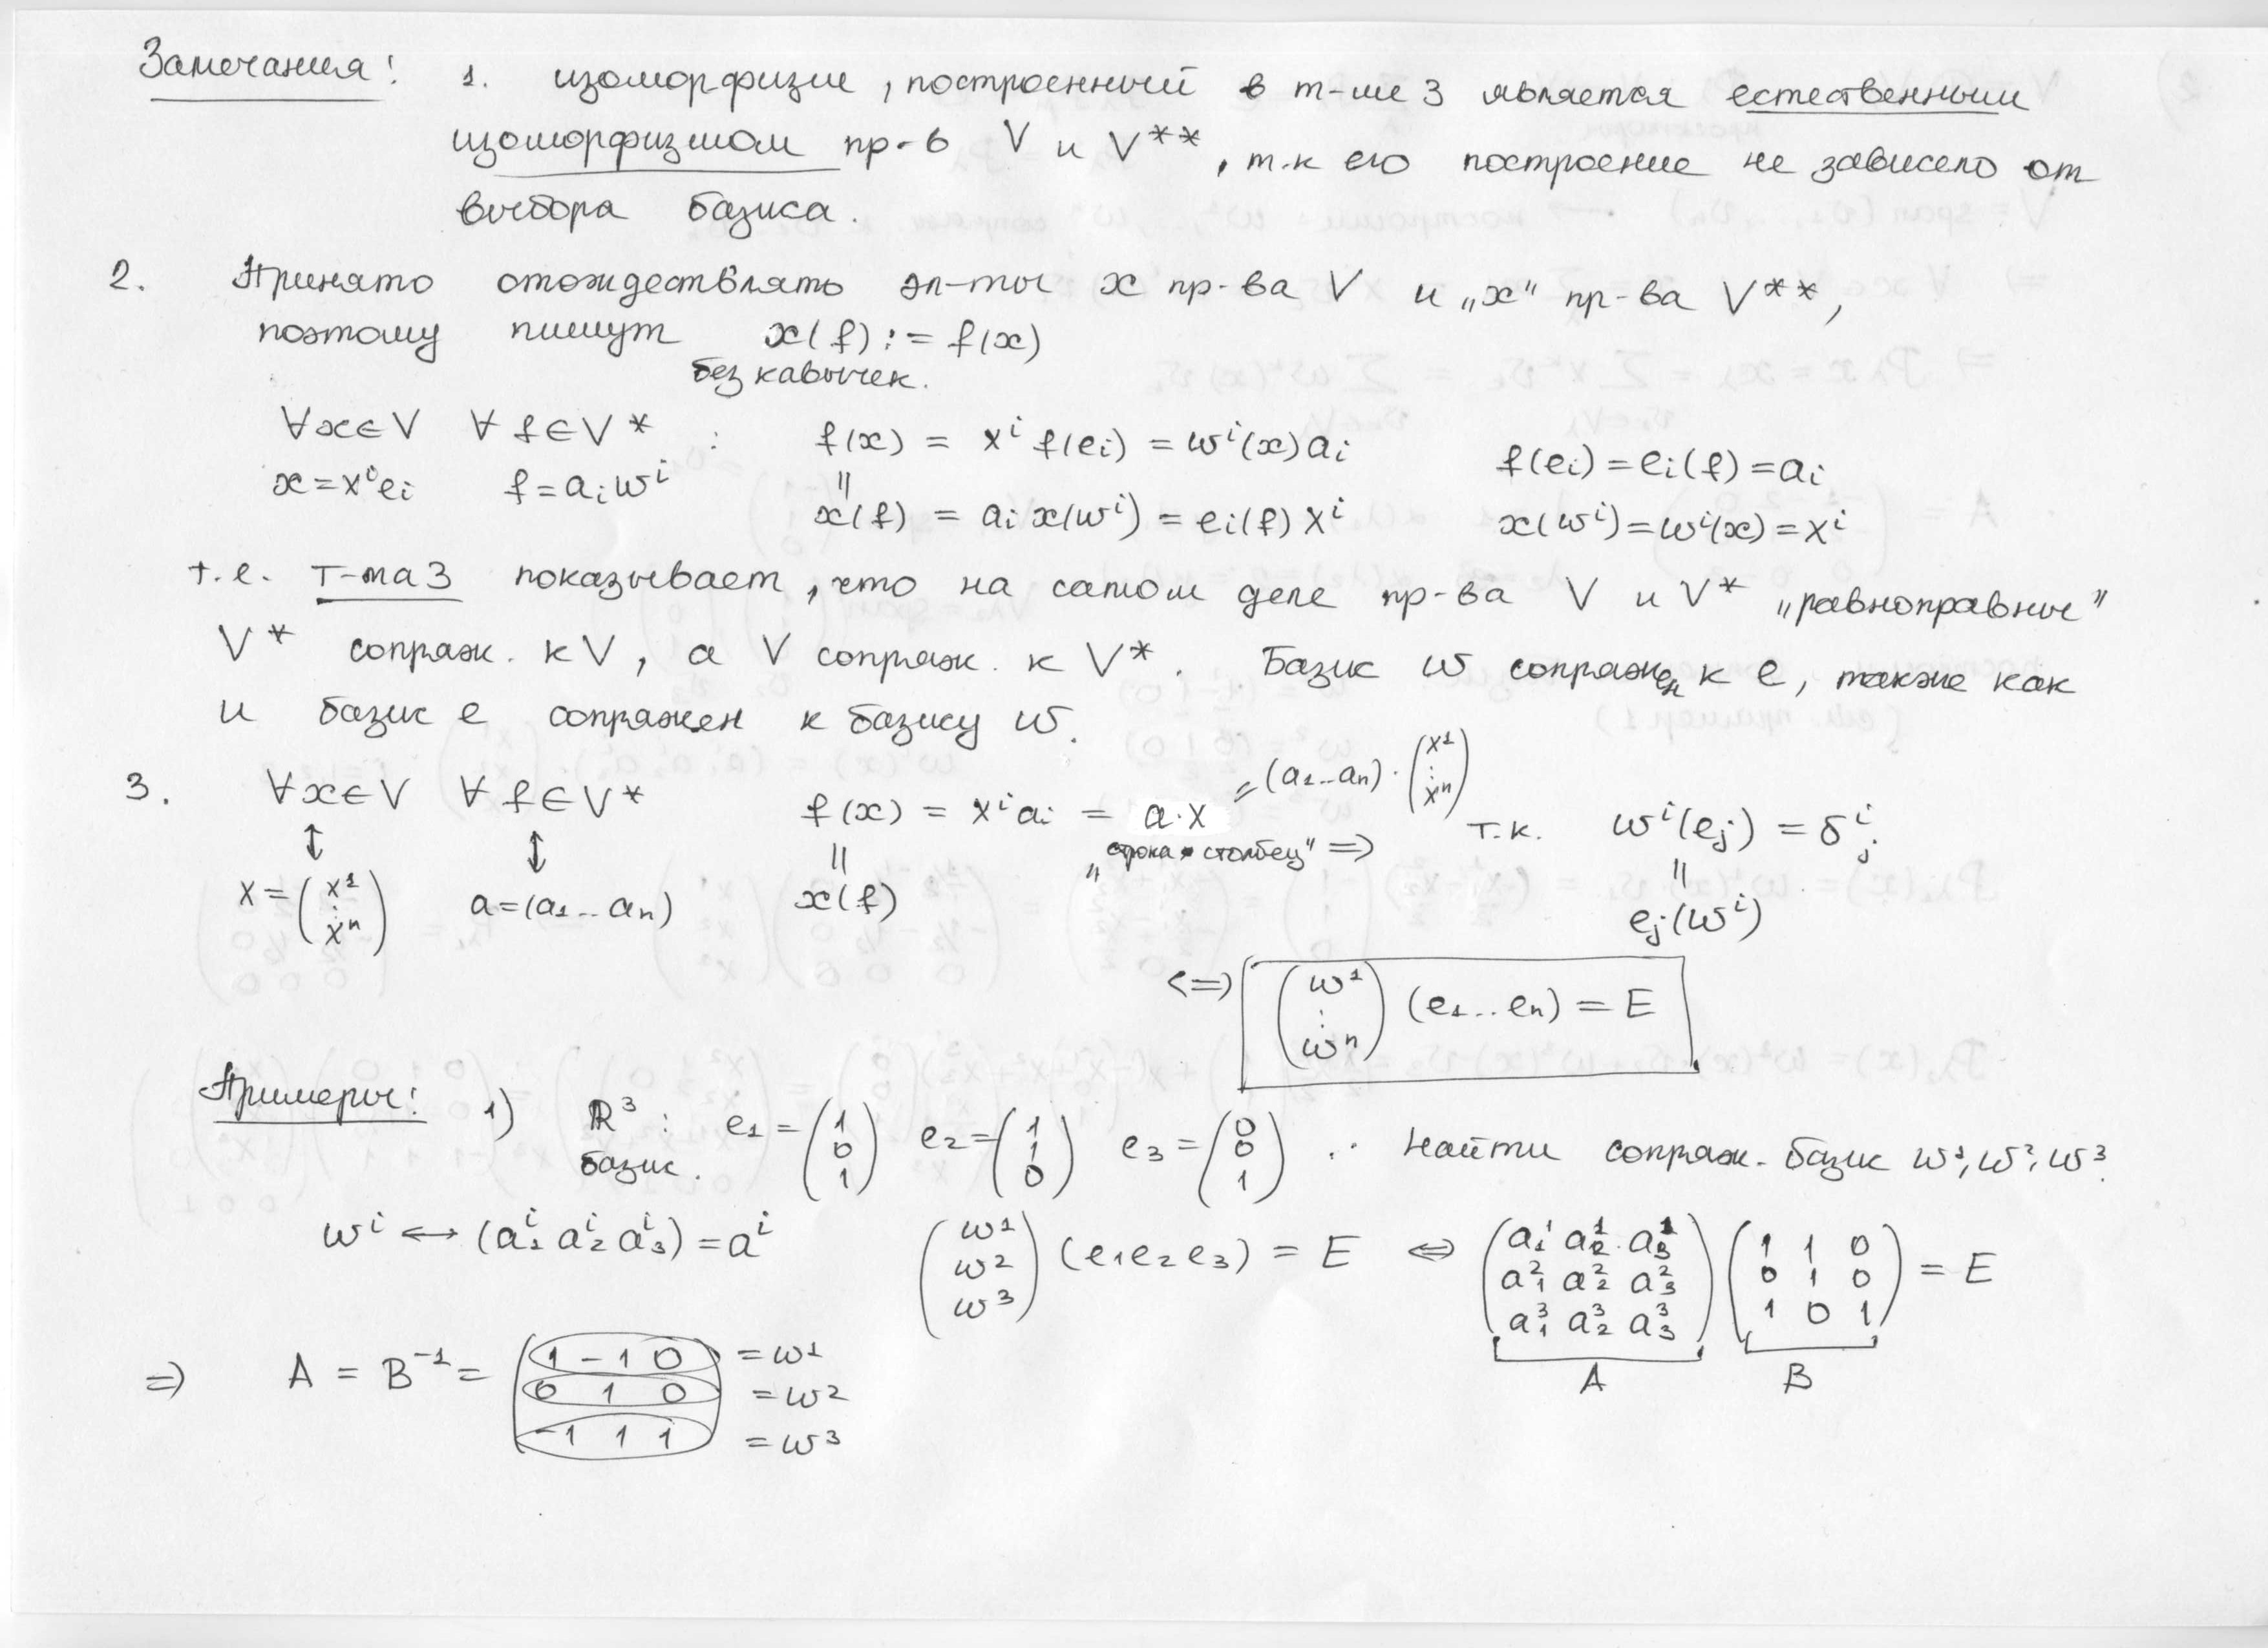
\includegraphics[height=0.49\textheight, width=\textwidth]{8_1-5}	
		\n
		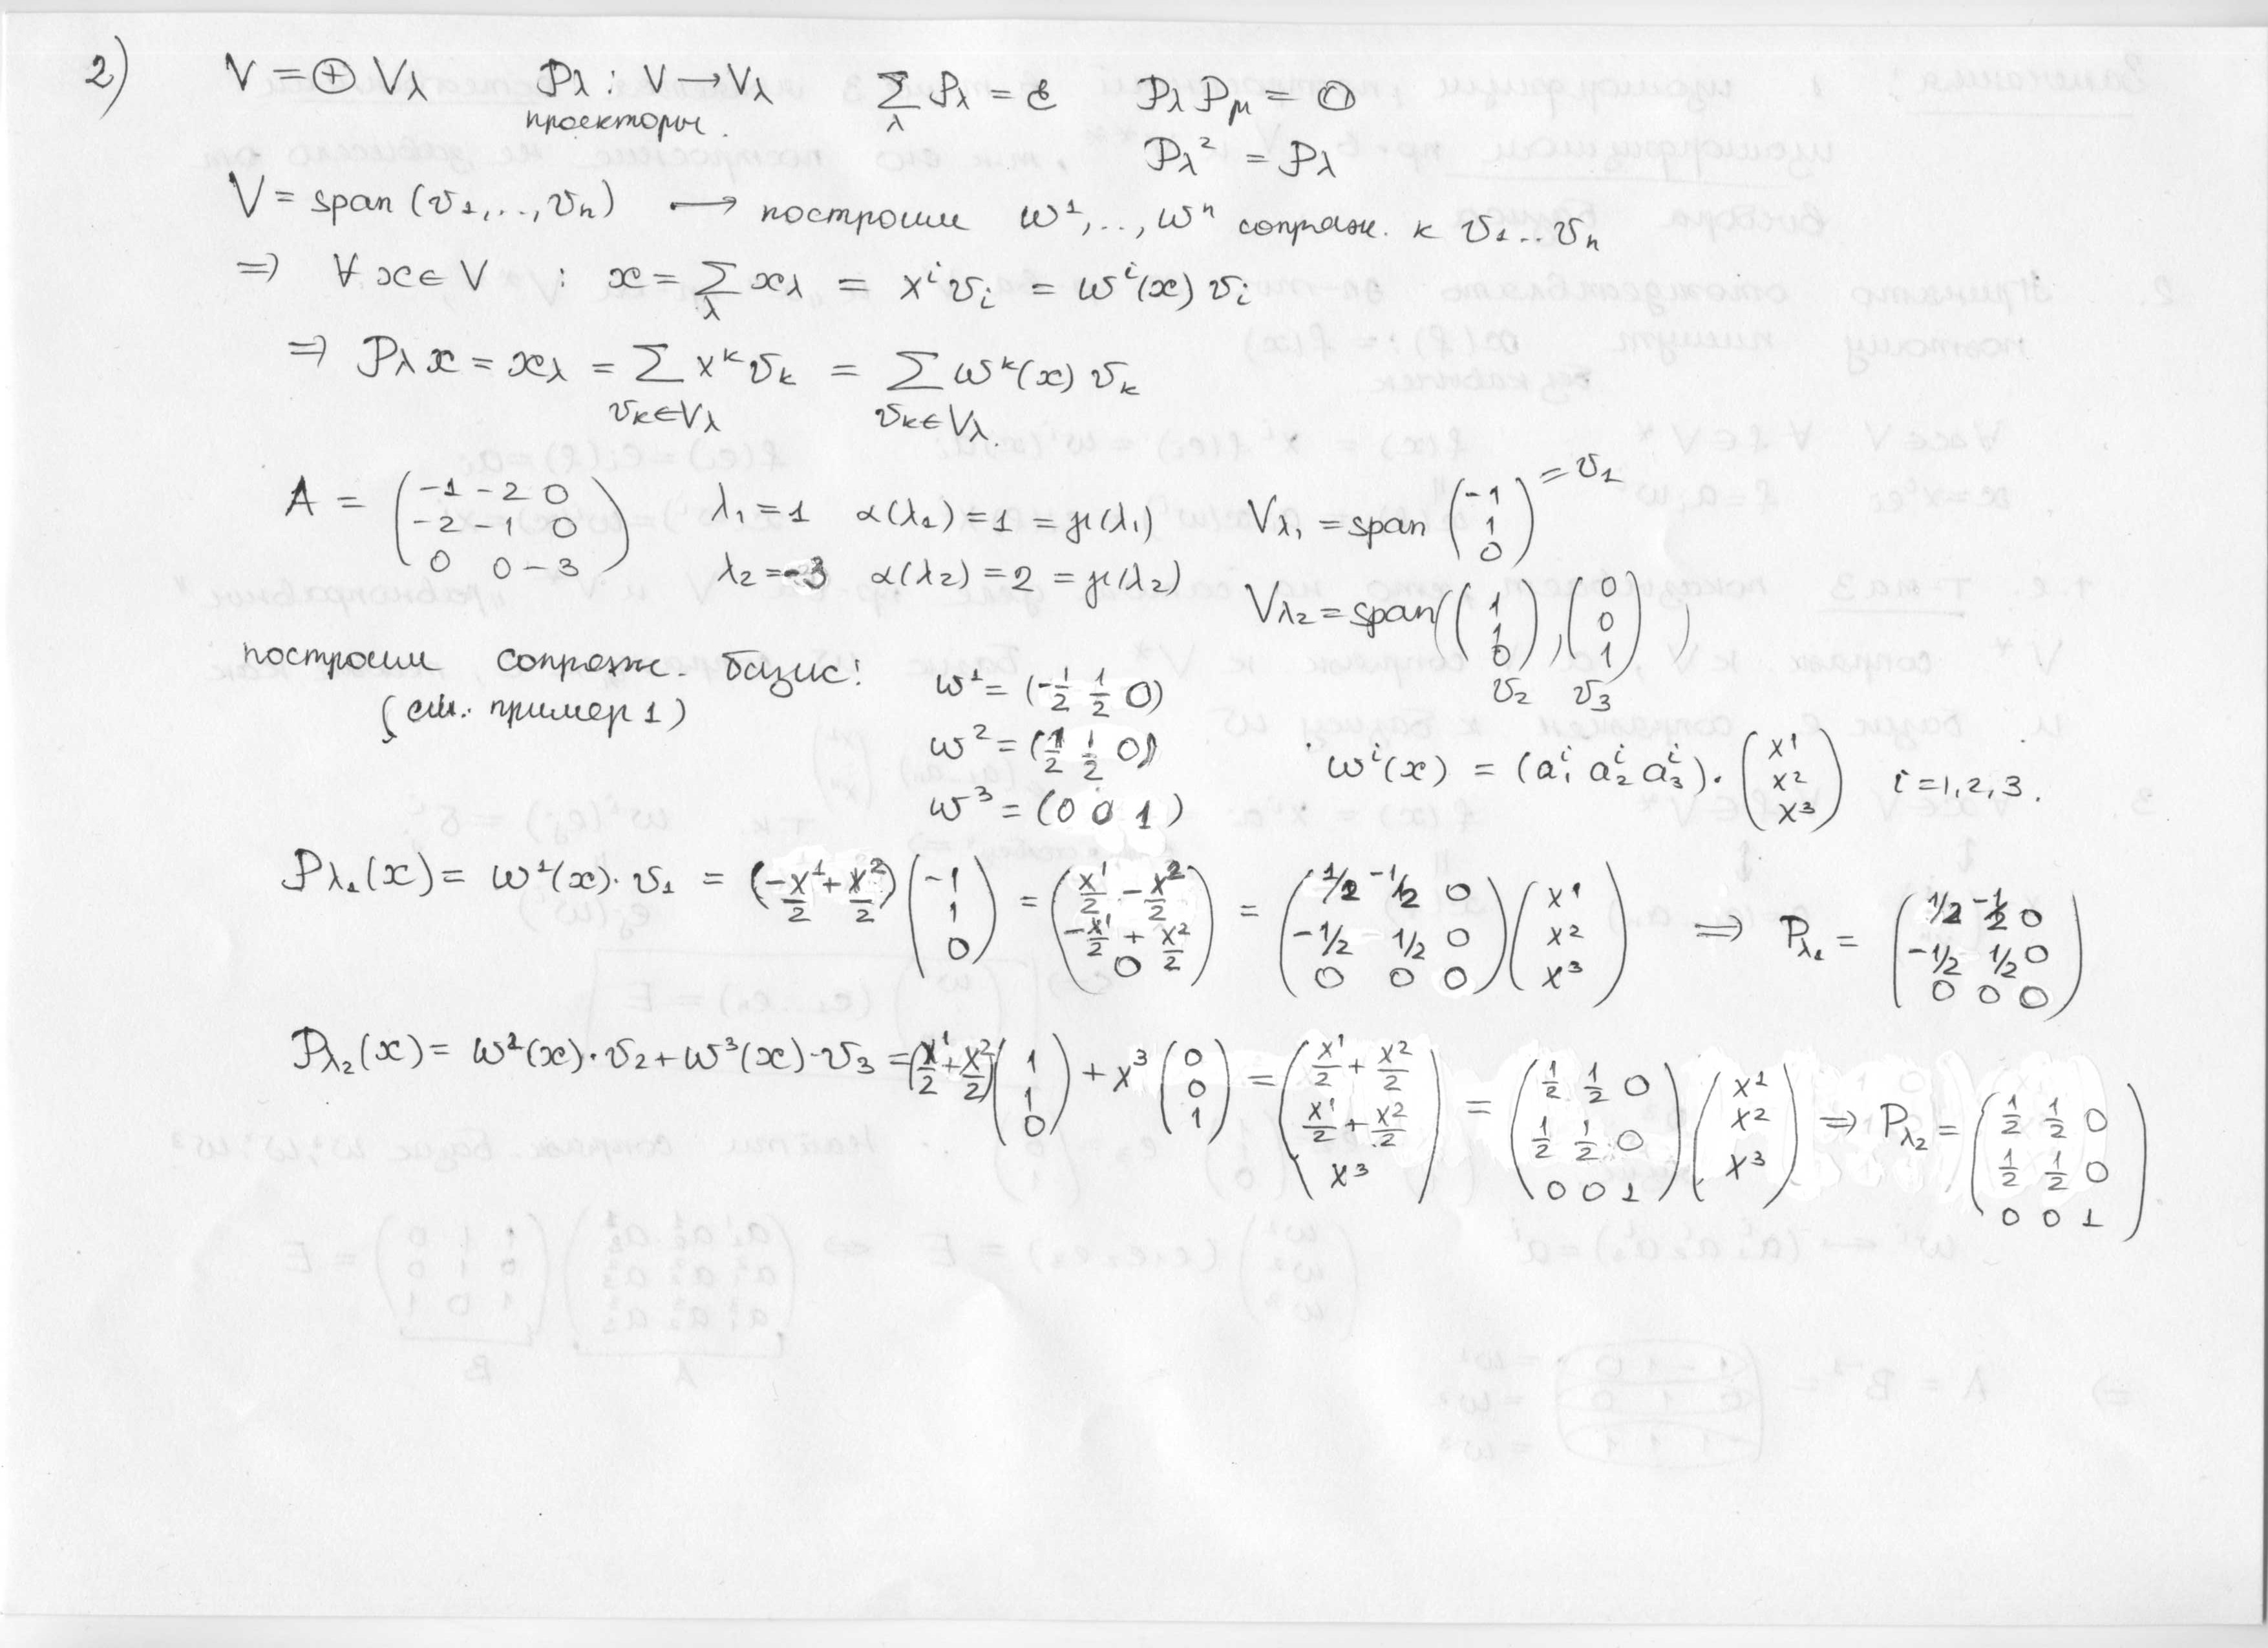
\includegraphics[height=0.49\textheight, width=\textwidth]{8_1-6}	
		\n
	\subsection{Два определения тензора. Многомерная матрица. Линейной пространство тензоров.}
	 		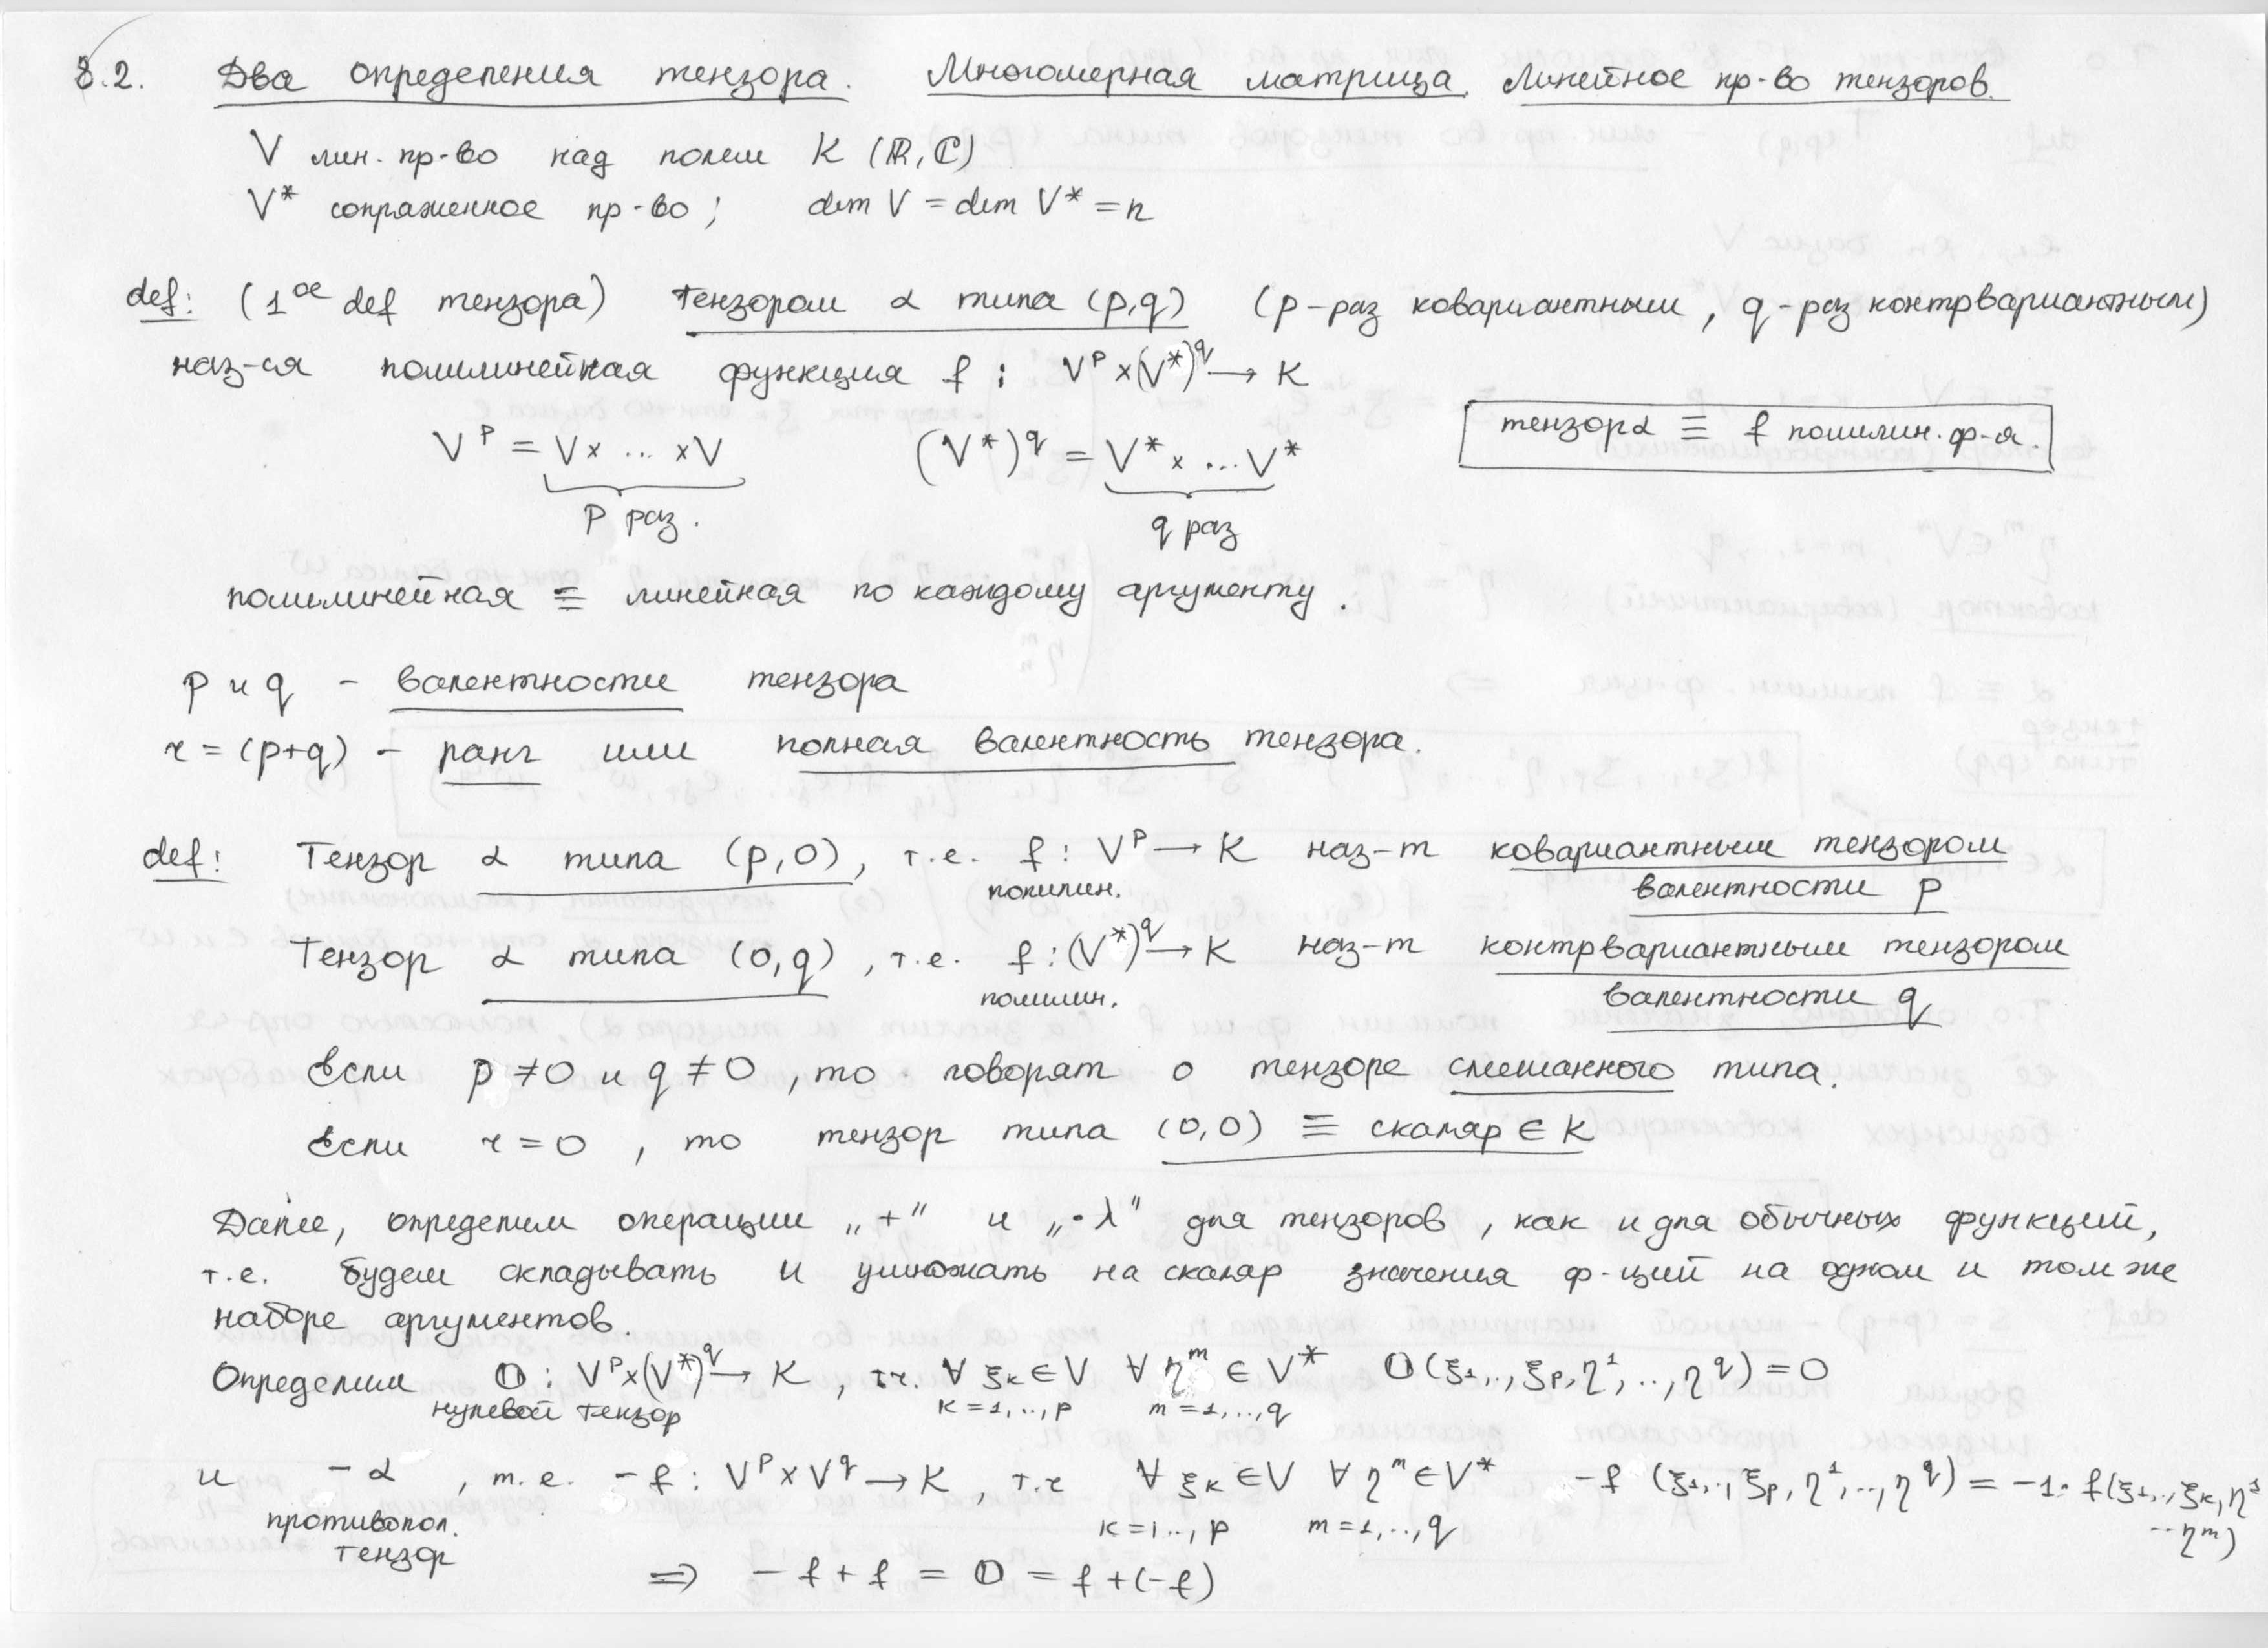
\includegraphics[height=0.49\textheight, width=\textwidth]{8_2-1}	
		\n
		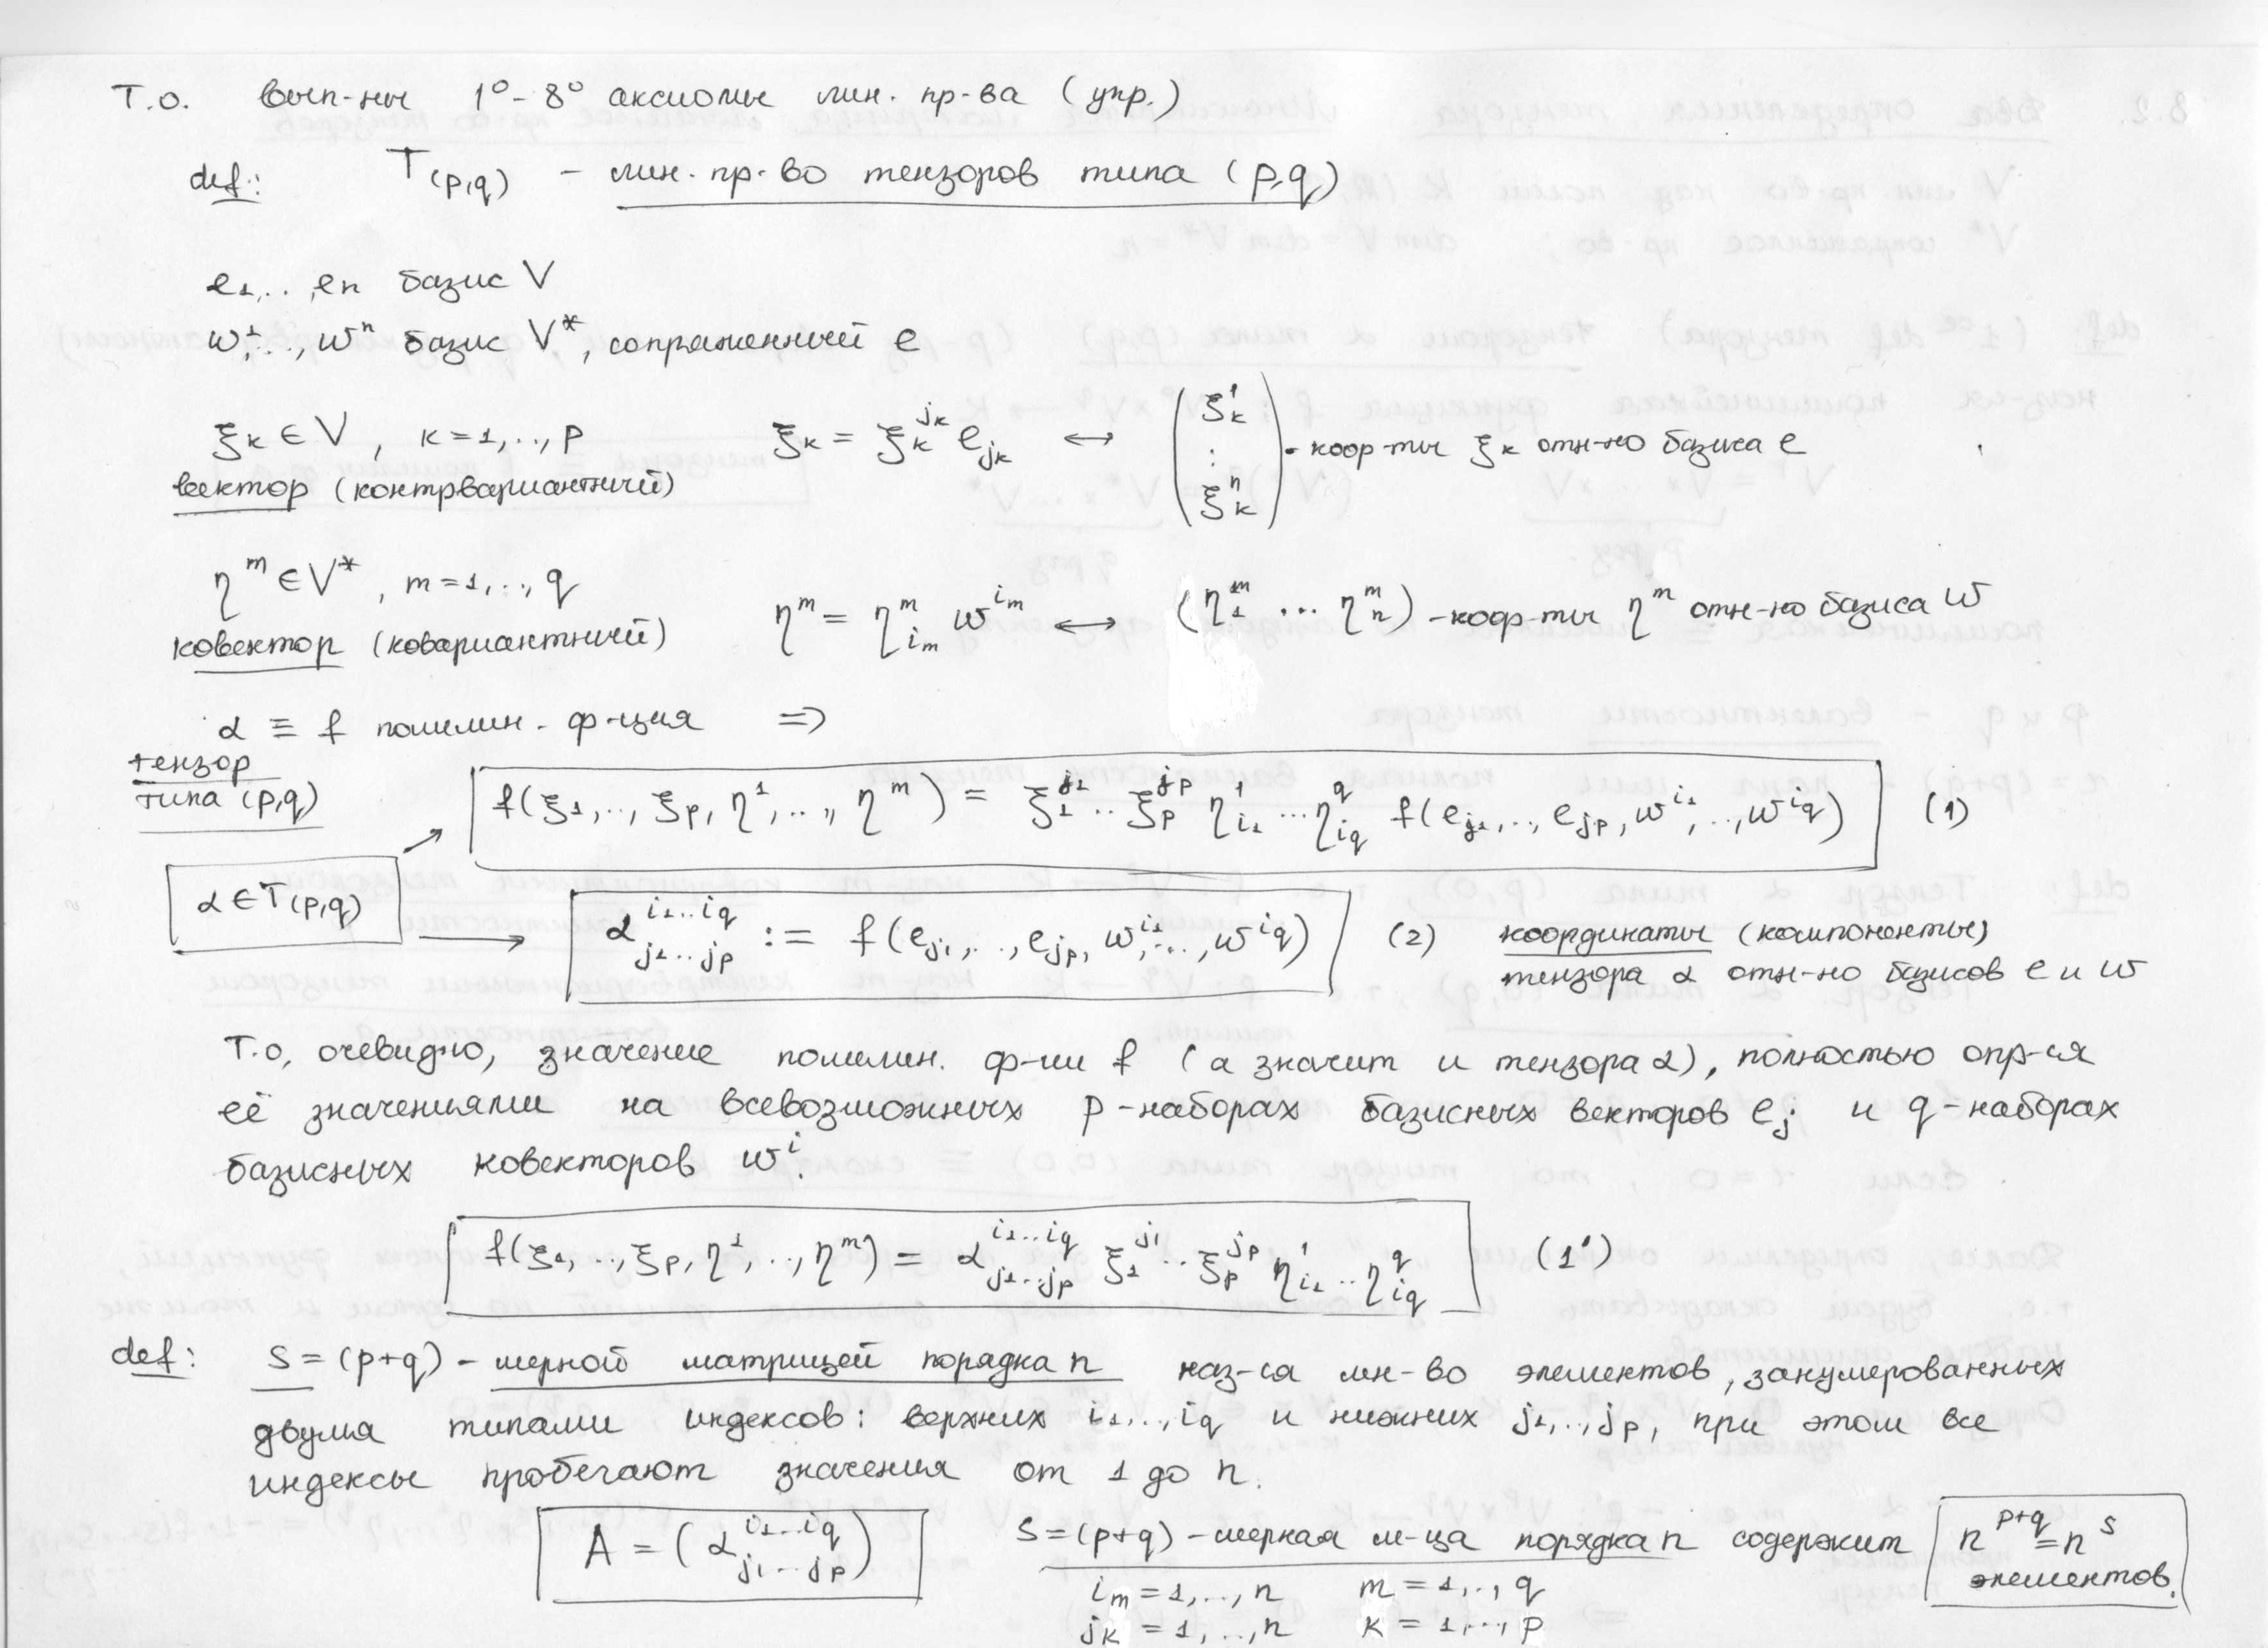
\includegraphics[height=0.49\textheight, width=\textwidth]{8_2-2}	
		\n
		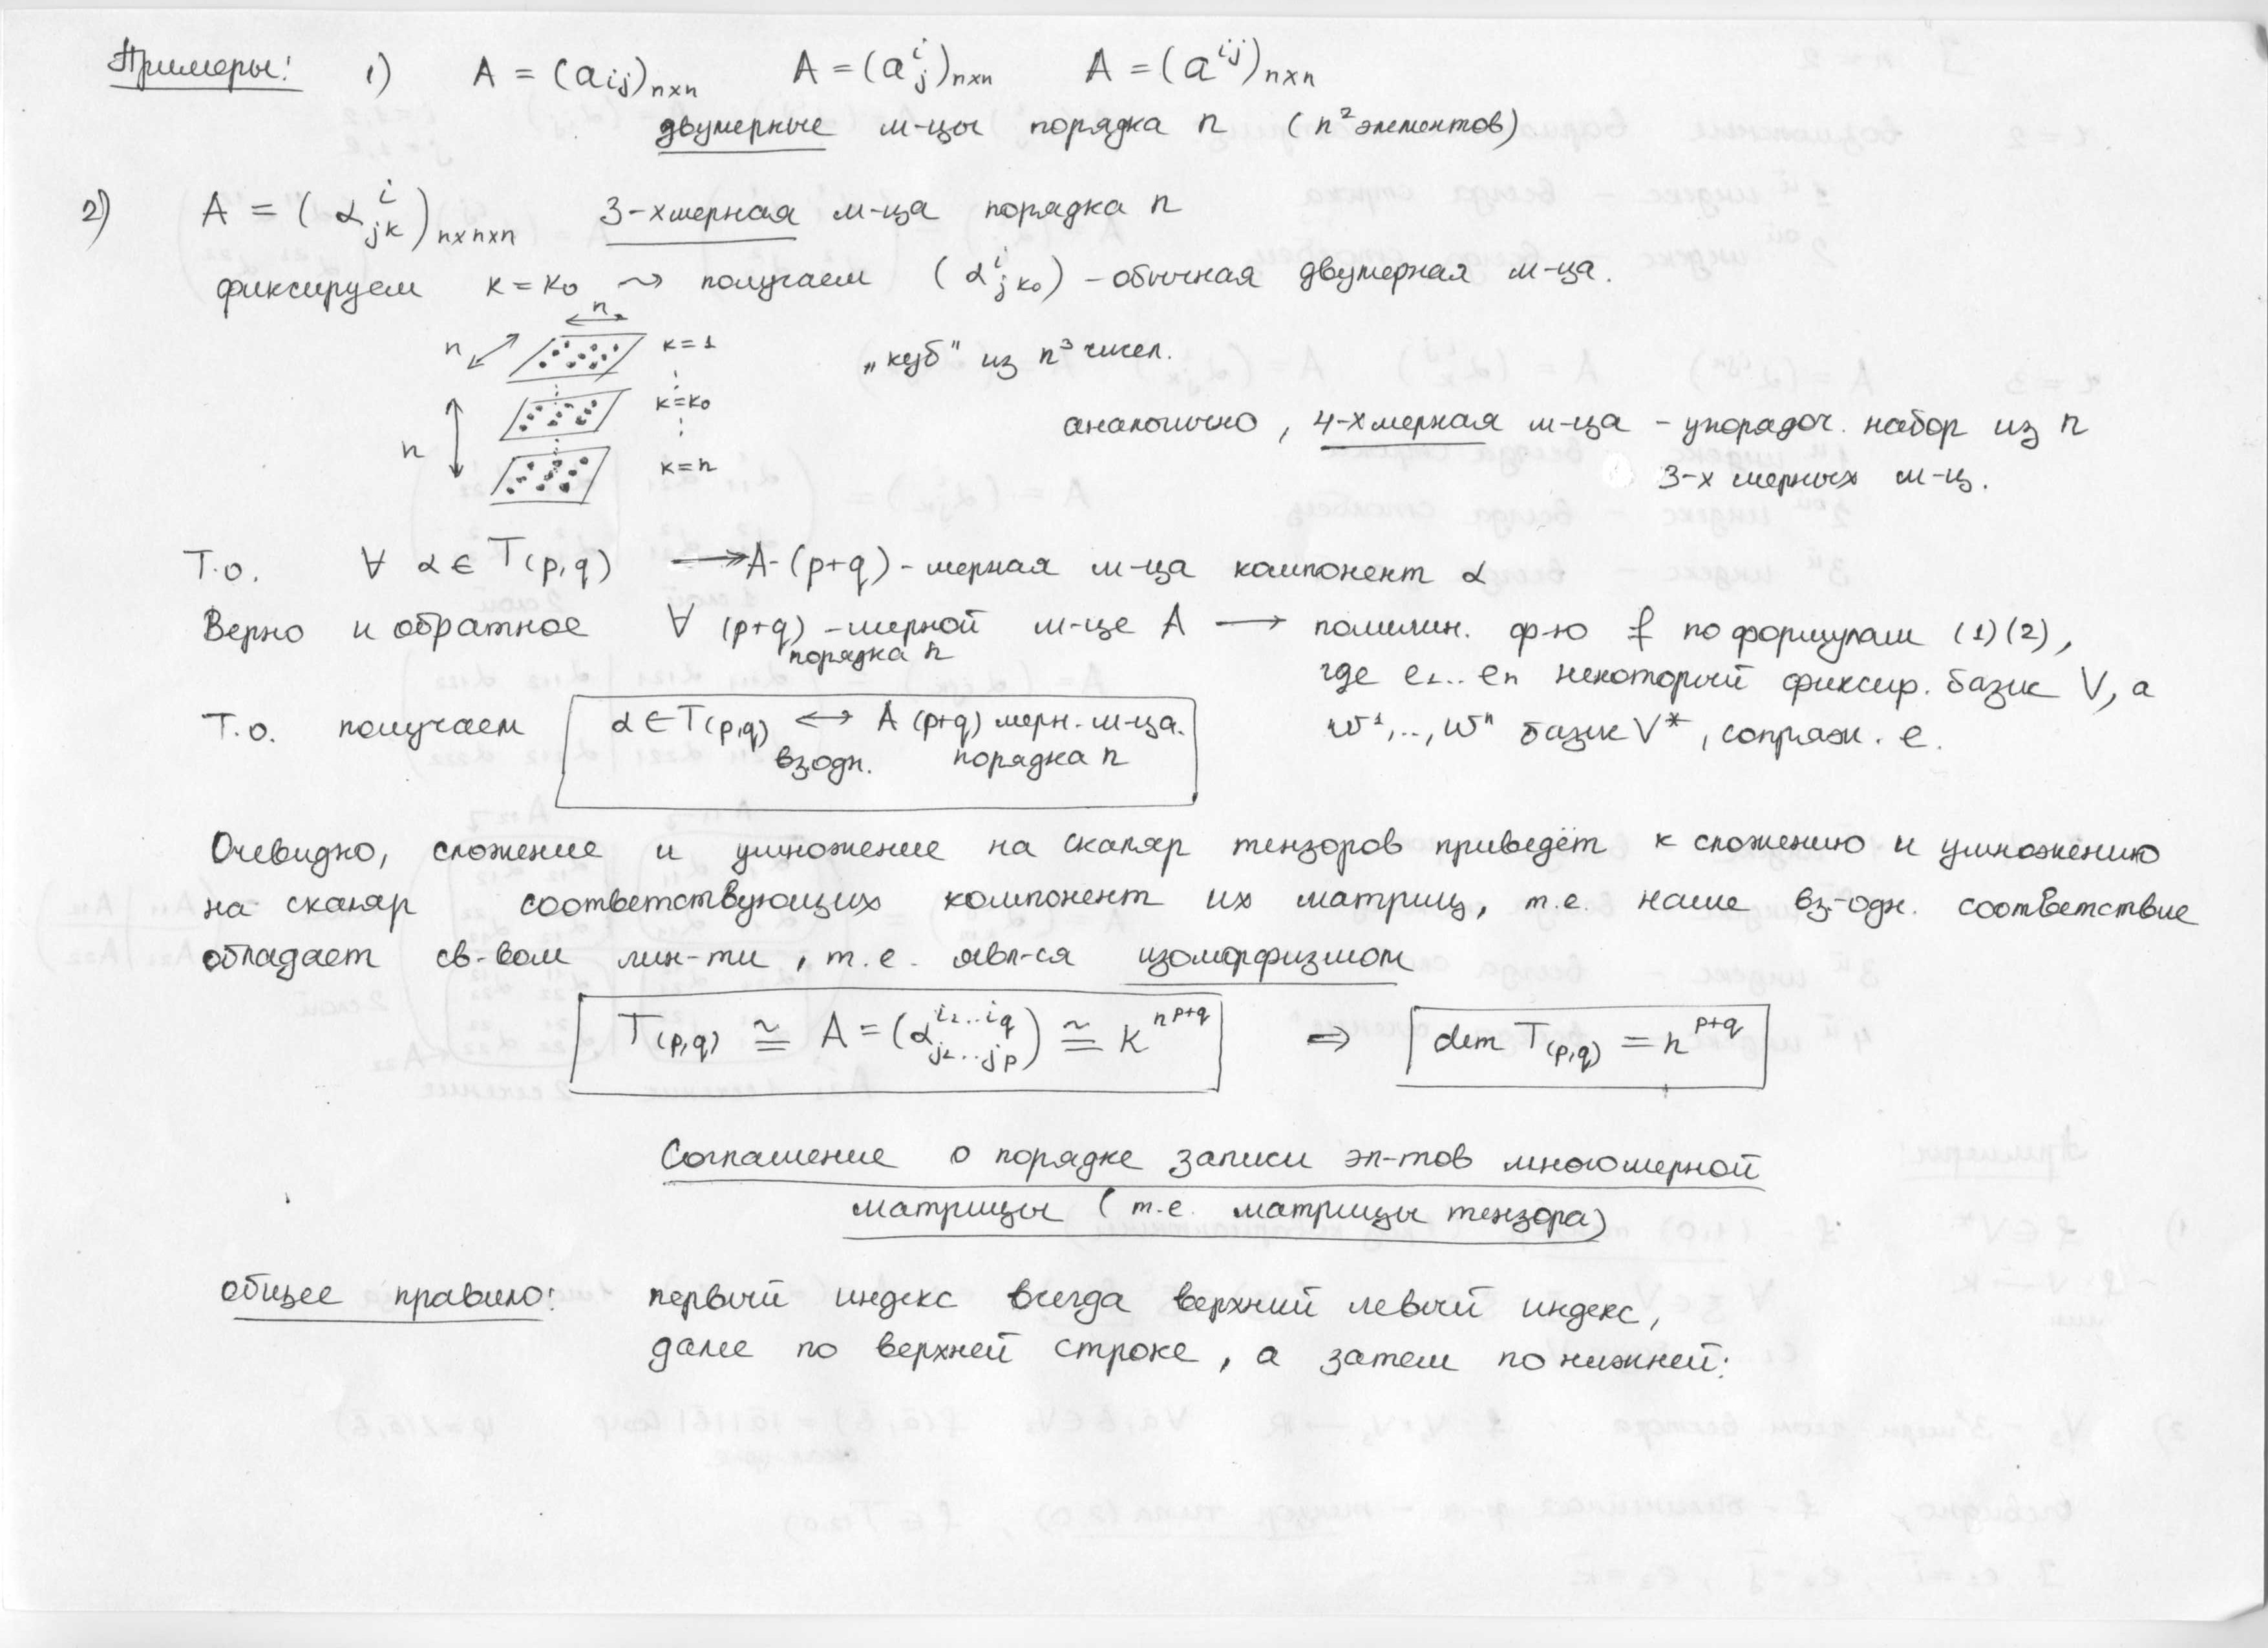
\includegraphics[height=0.49\textheight, width=\textwidth]{8_2-3}	
		\n
		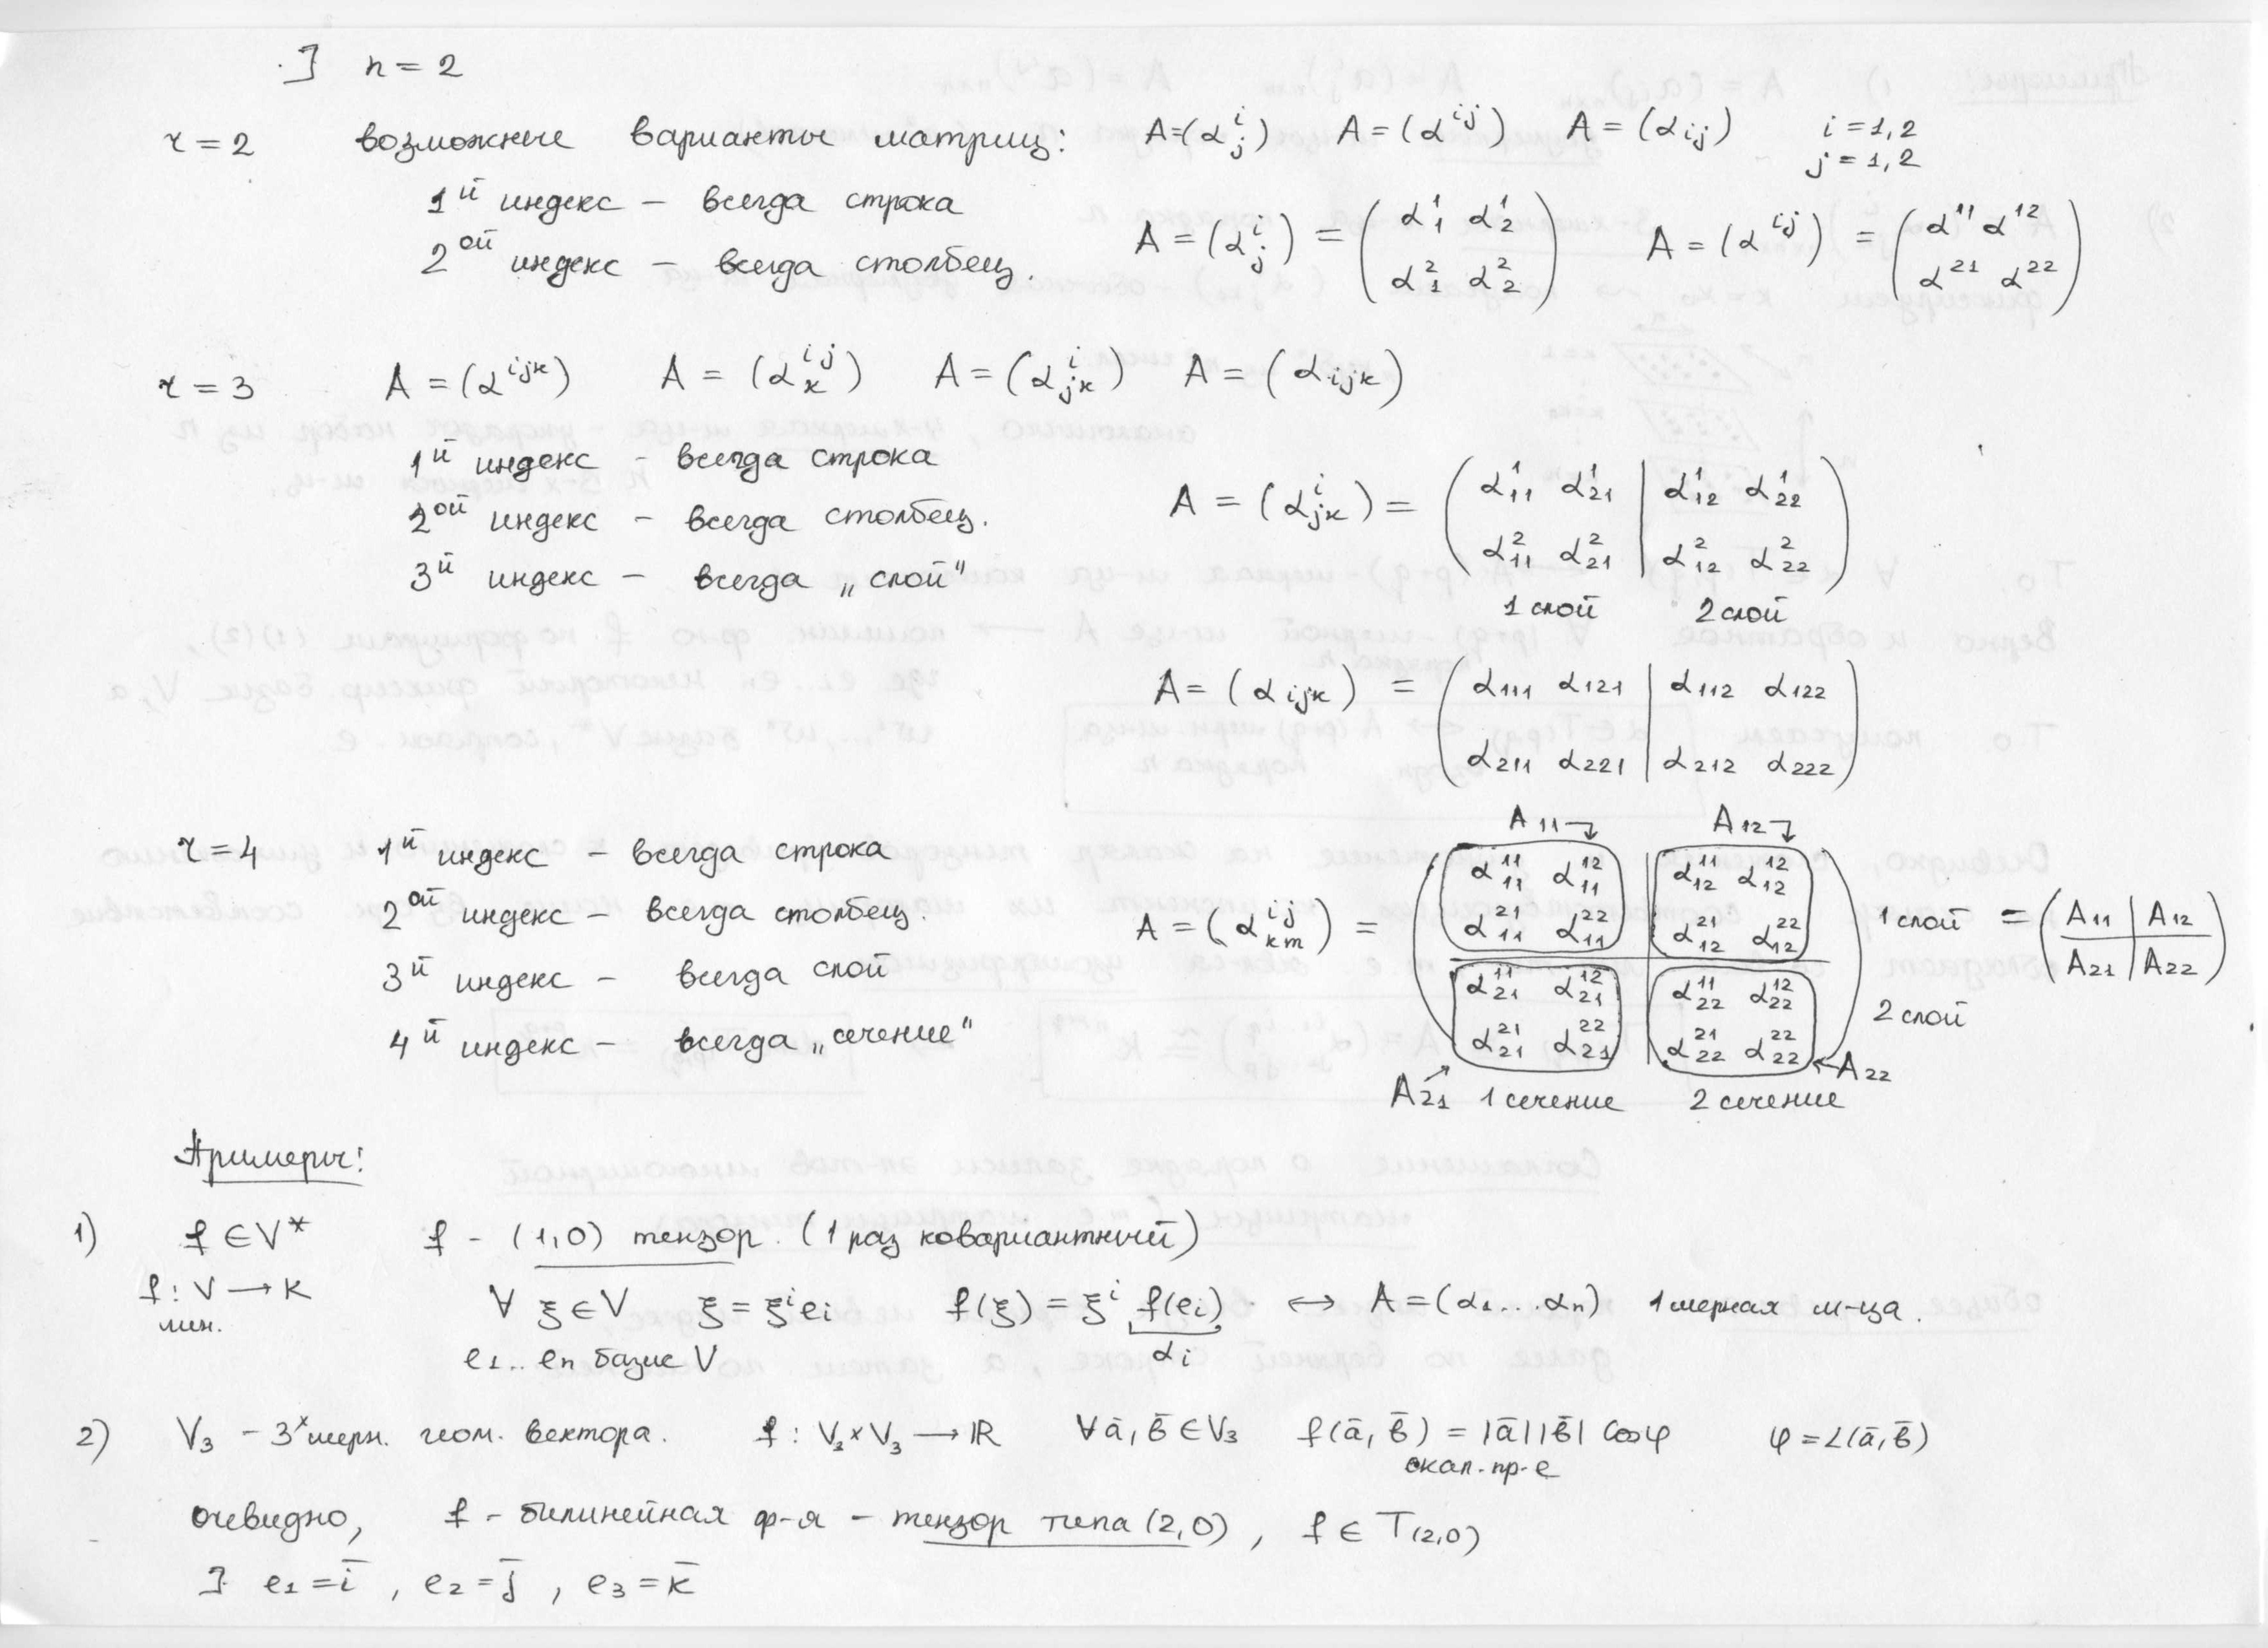
\includegraphics[height=0.49\textheight, width=\textwidth]{8_2-4}	
		\n
		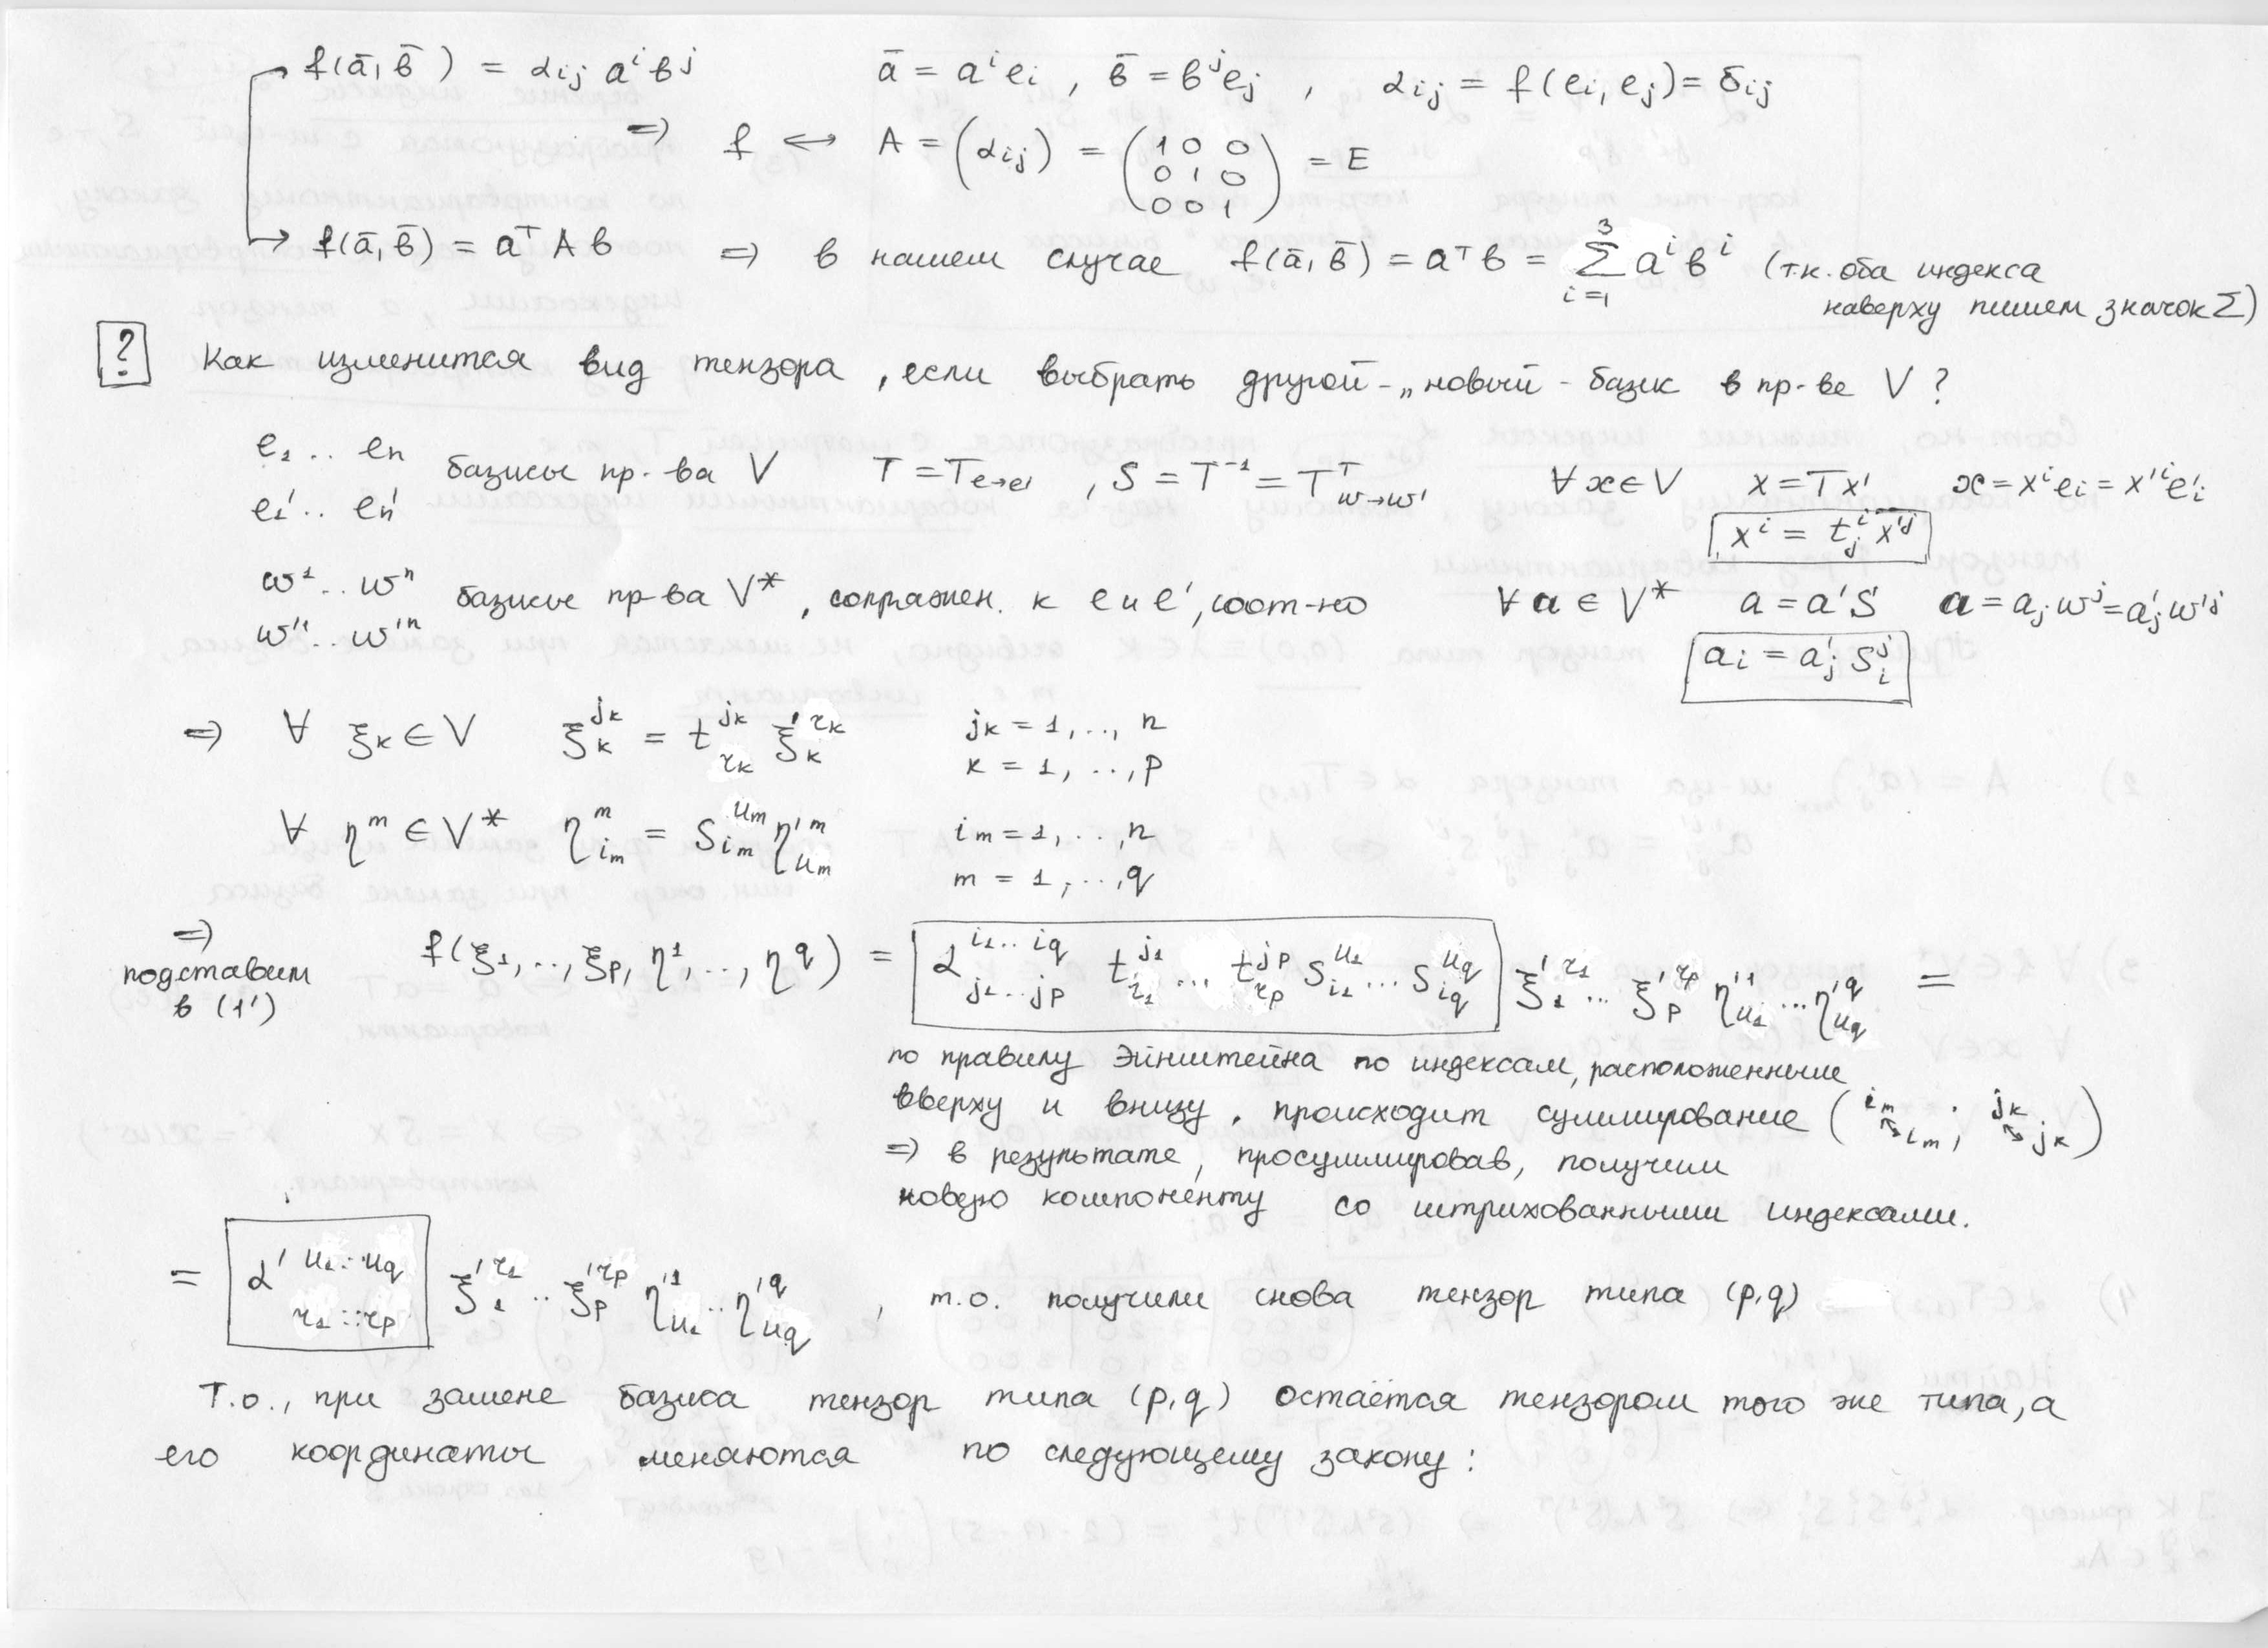
\includegraphics[height=0.49\textheight, width=\textwidth]{8_2-5}	
		\n
		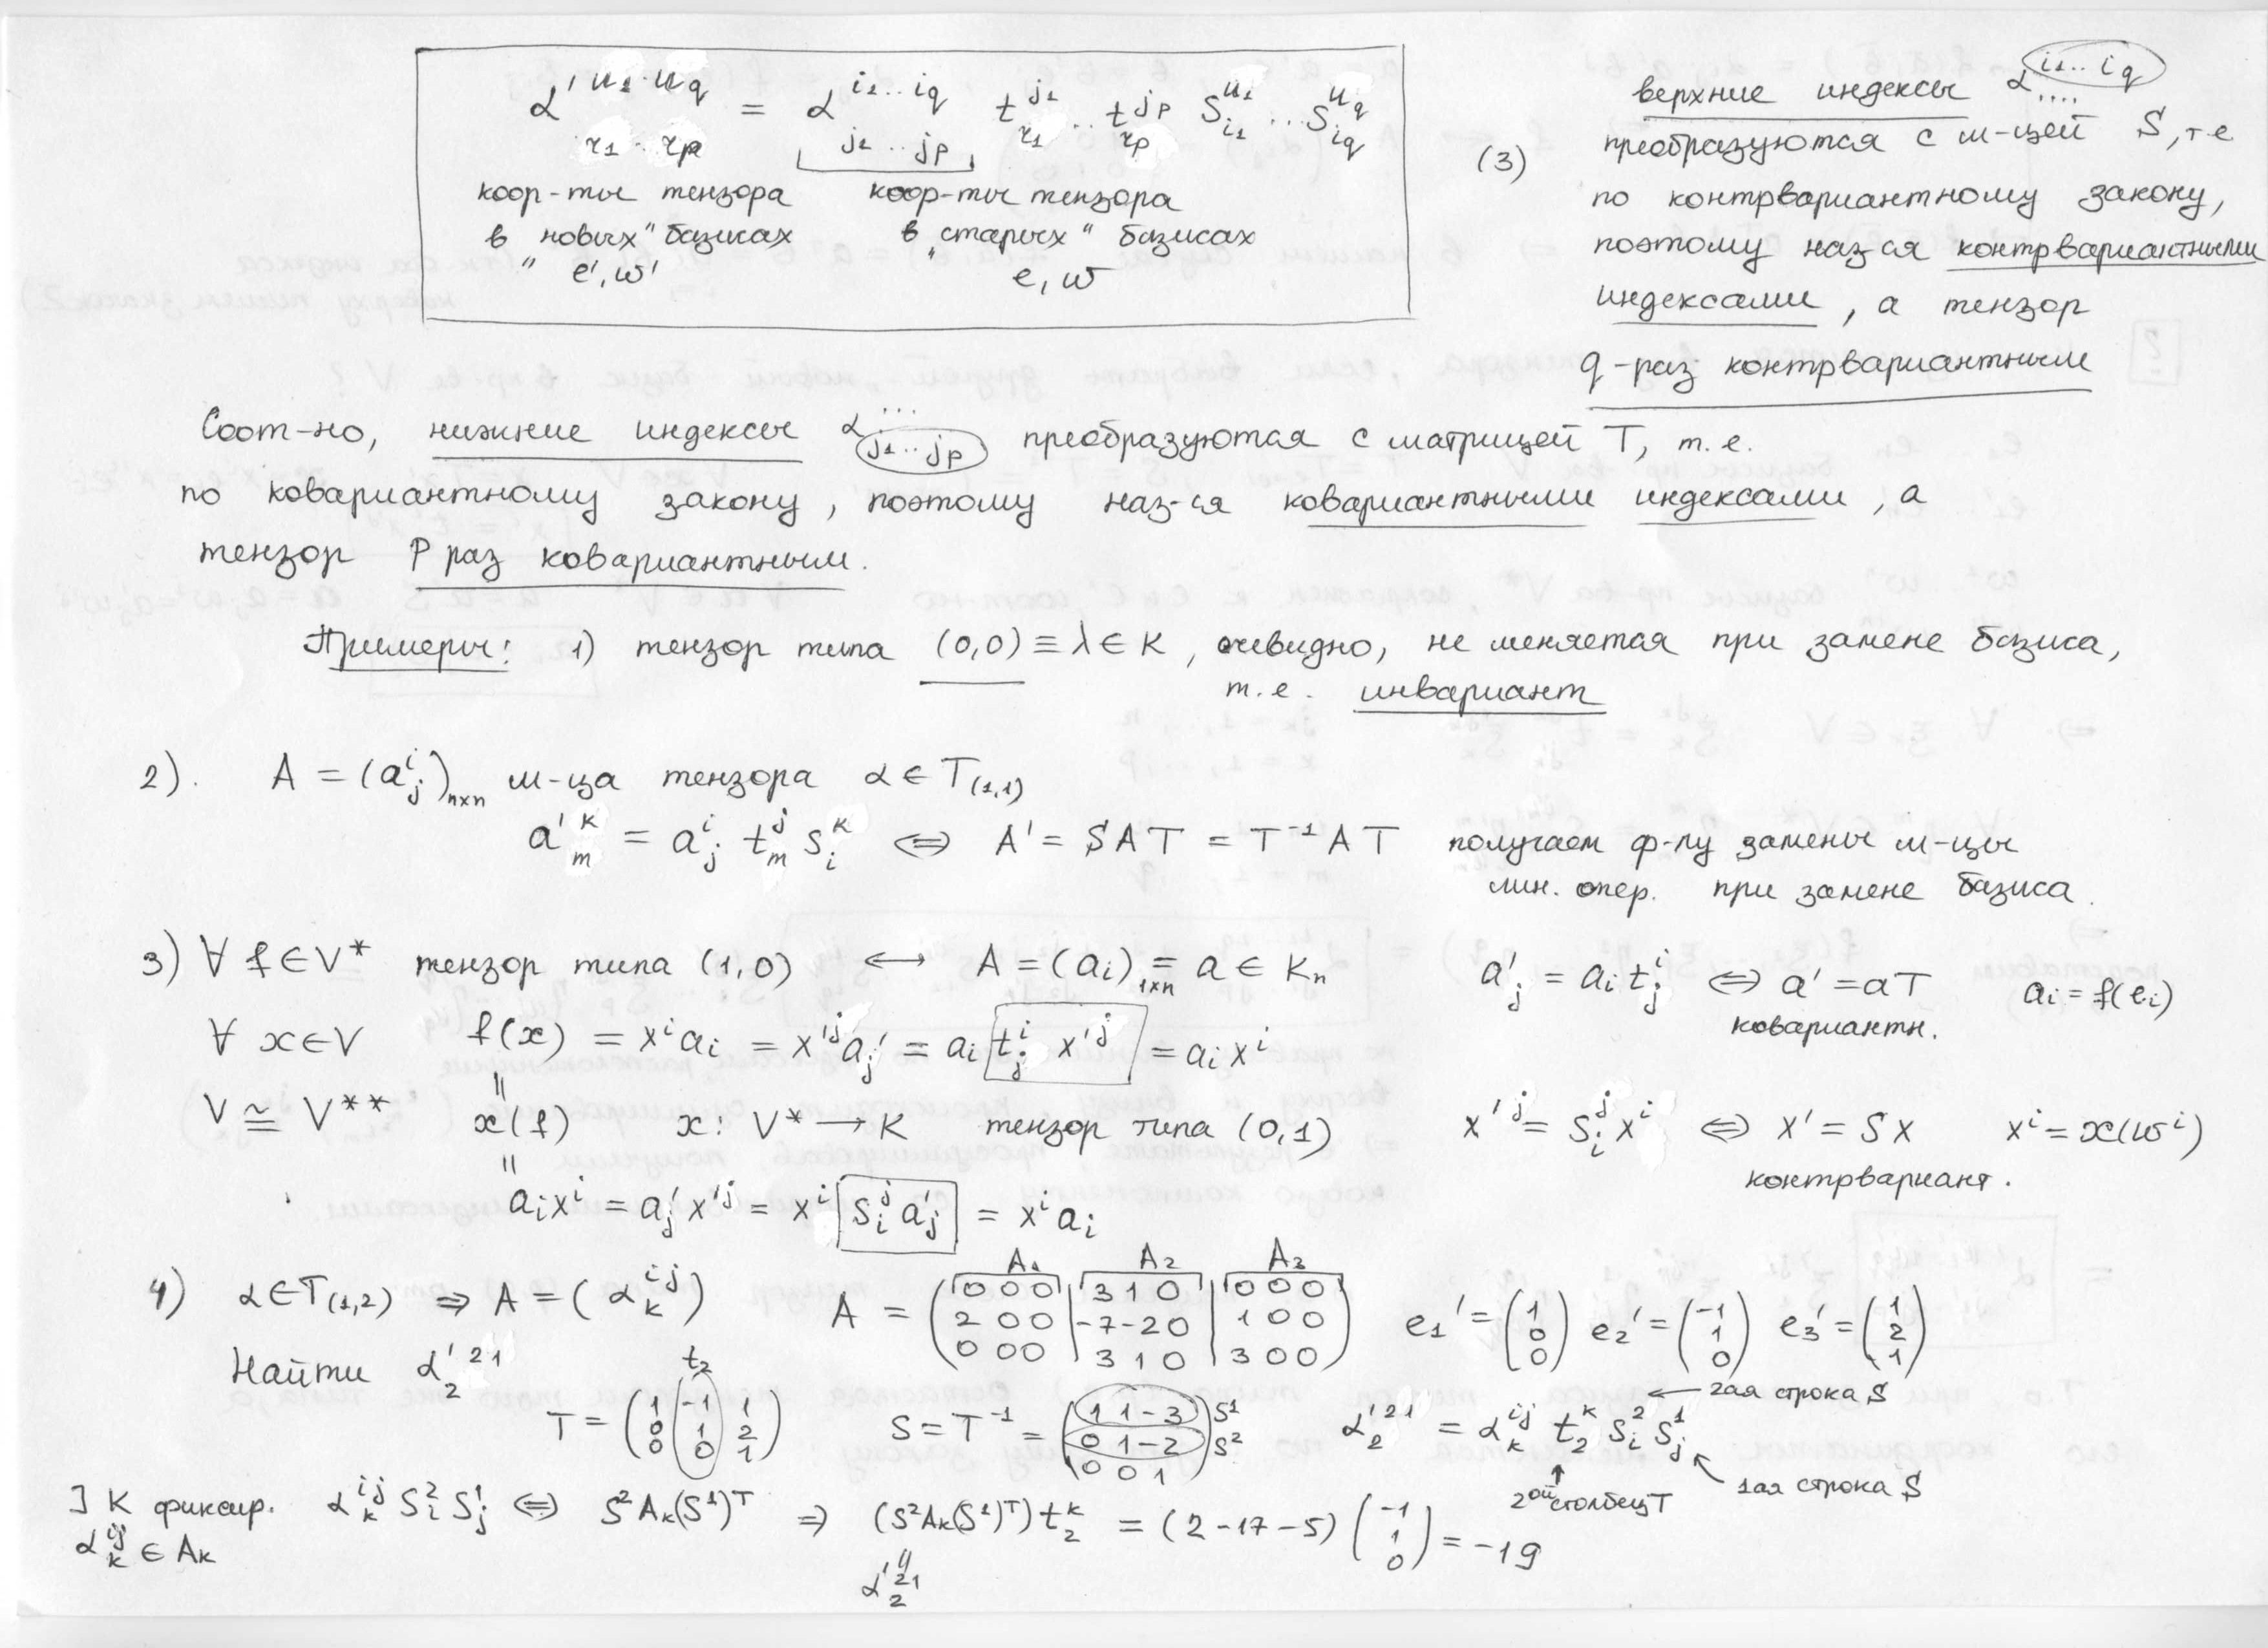
\includegraphics[height=0.49\textheight, width=\textwidth]{8_2-6}	
		\n
		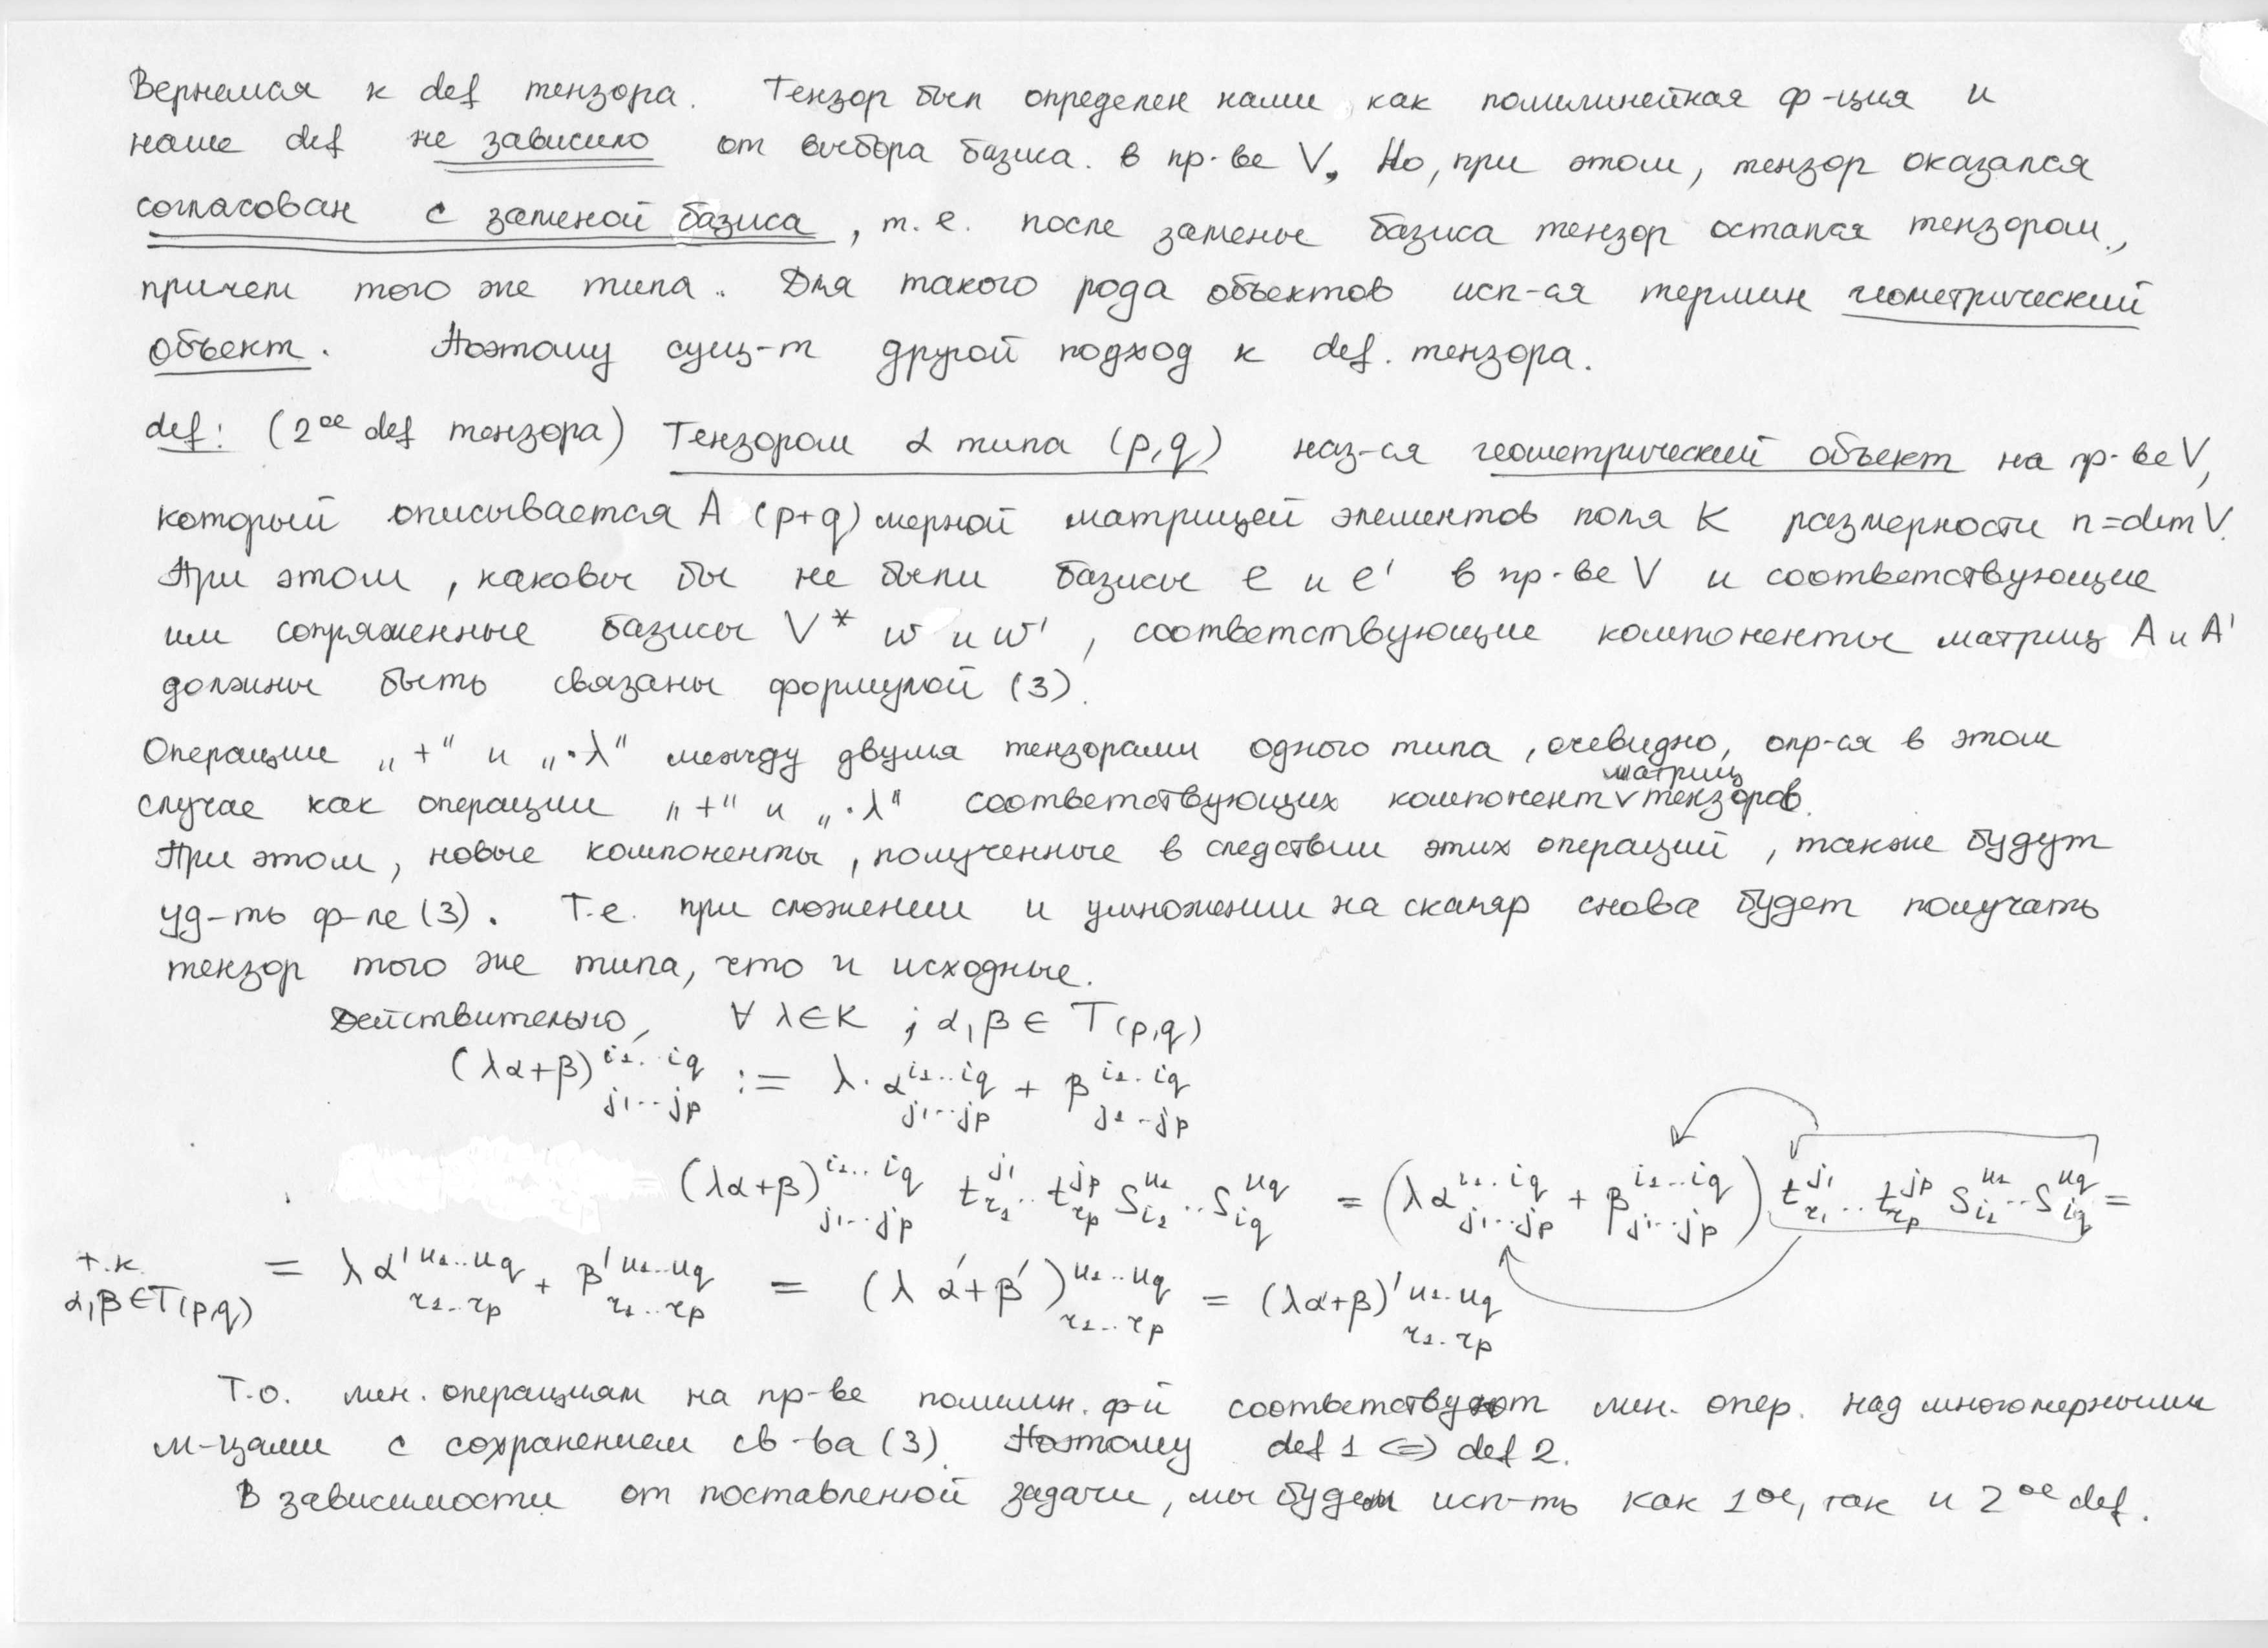
\includegraphics[height=0.49\textheight, width=\textwidth]{8_2-7}	
		
		
	\subsection{Произведение тензоров. Базис пространства тензоров. Операция свертки.}
	 		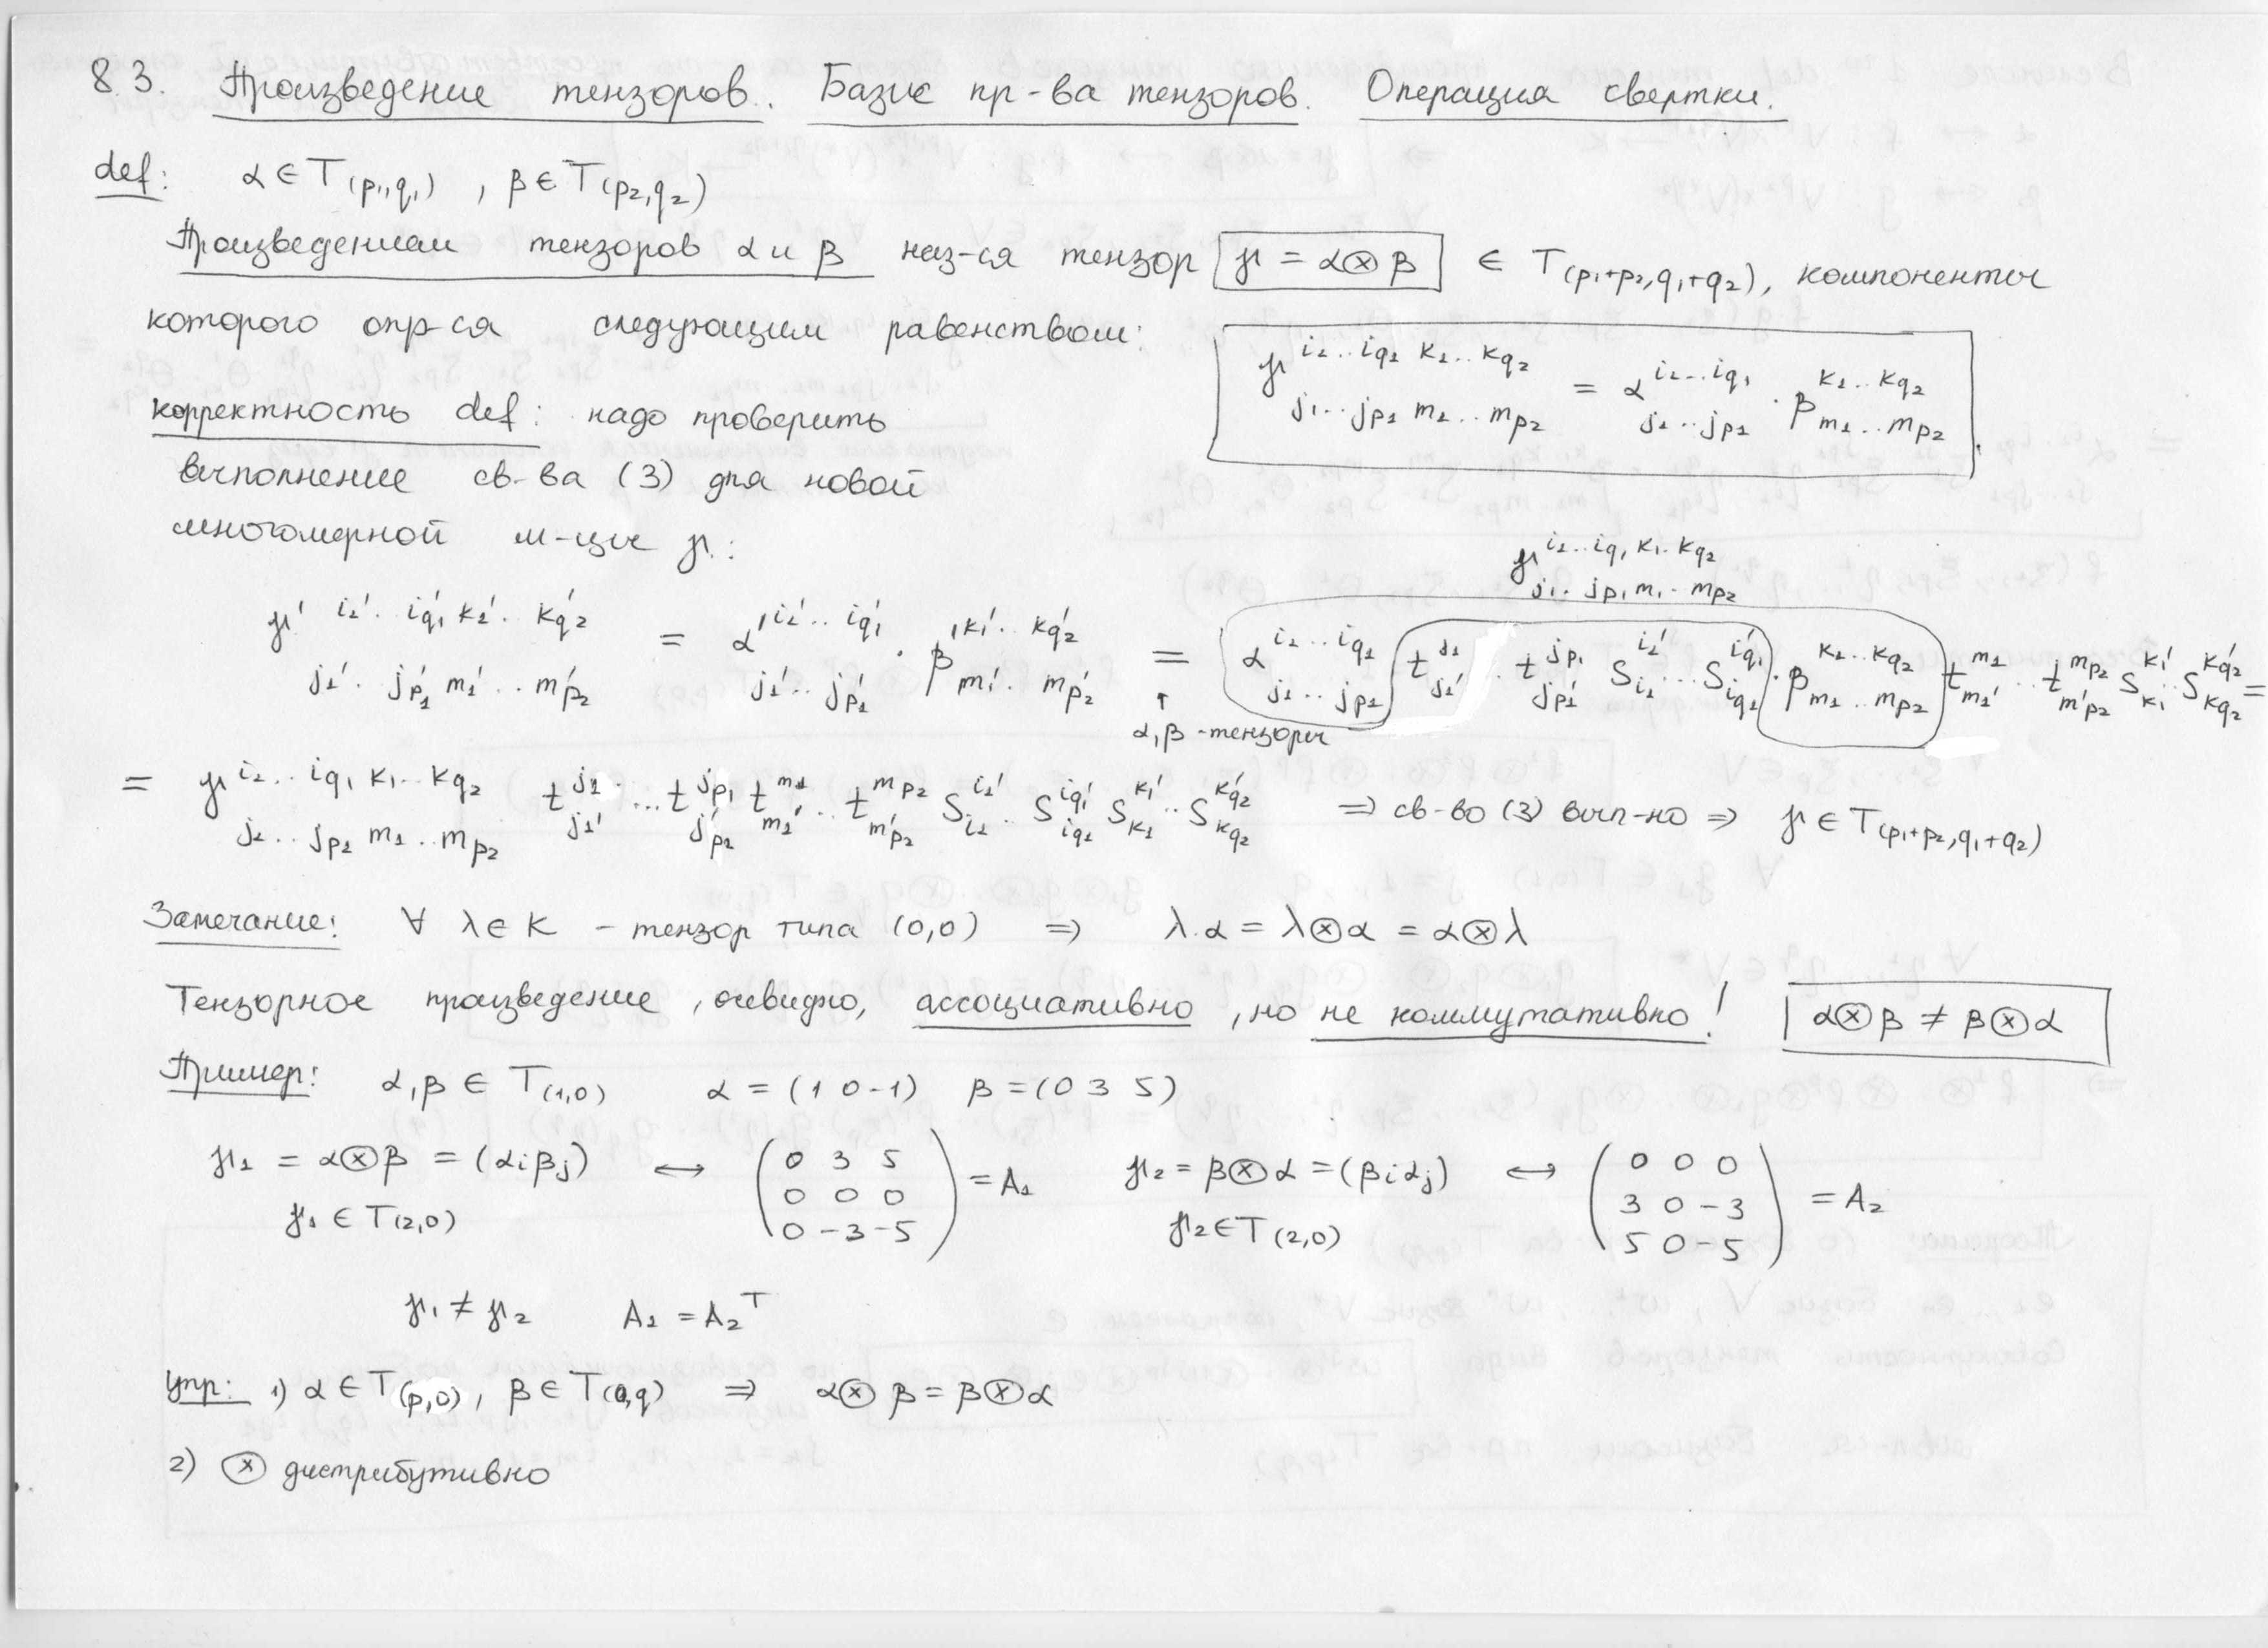
\includegraphics[height=0.49\textheight, width=\textwidth]{03001}	
		\n
		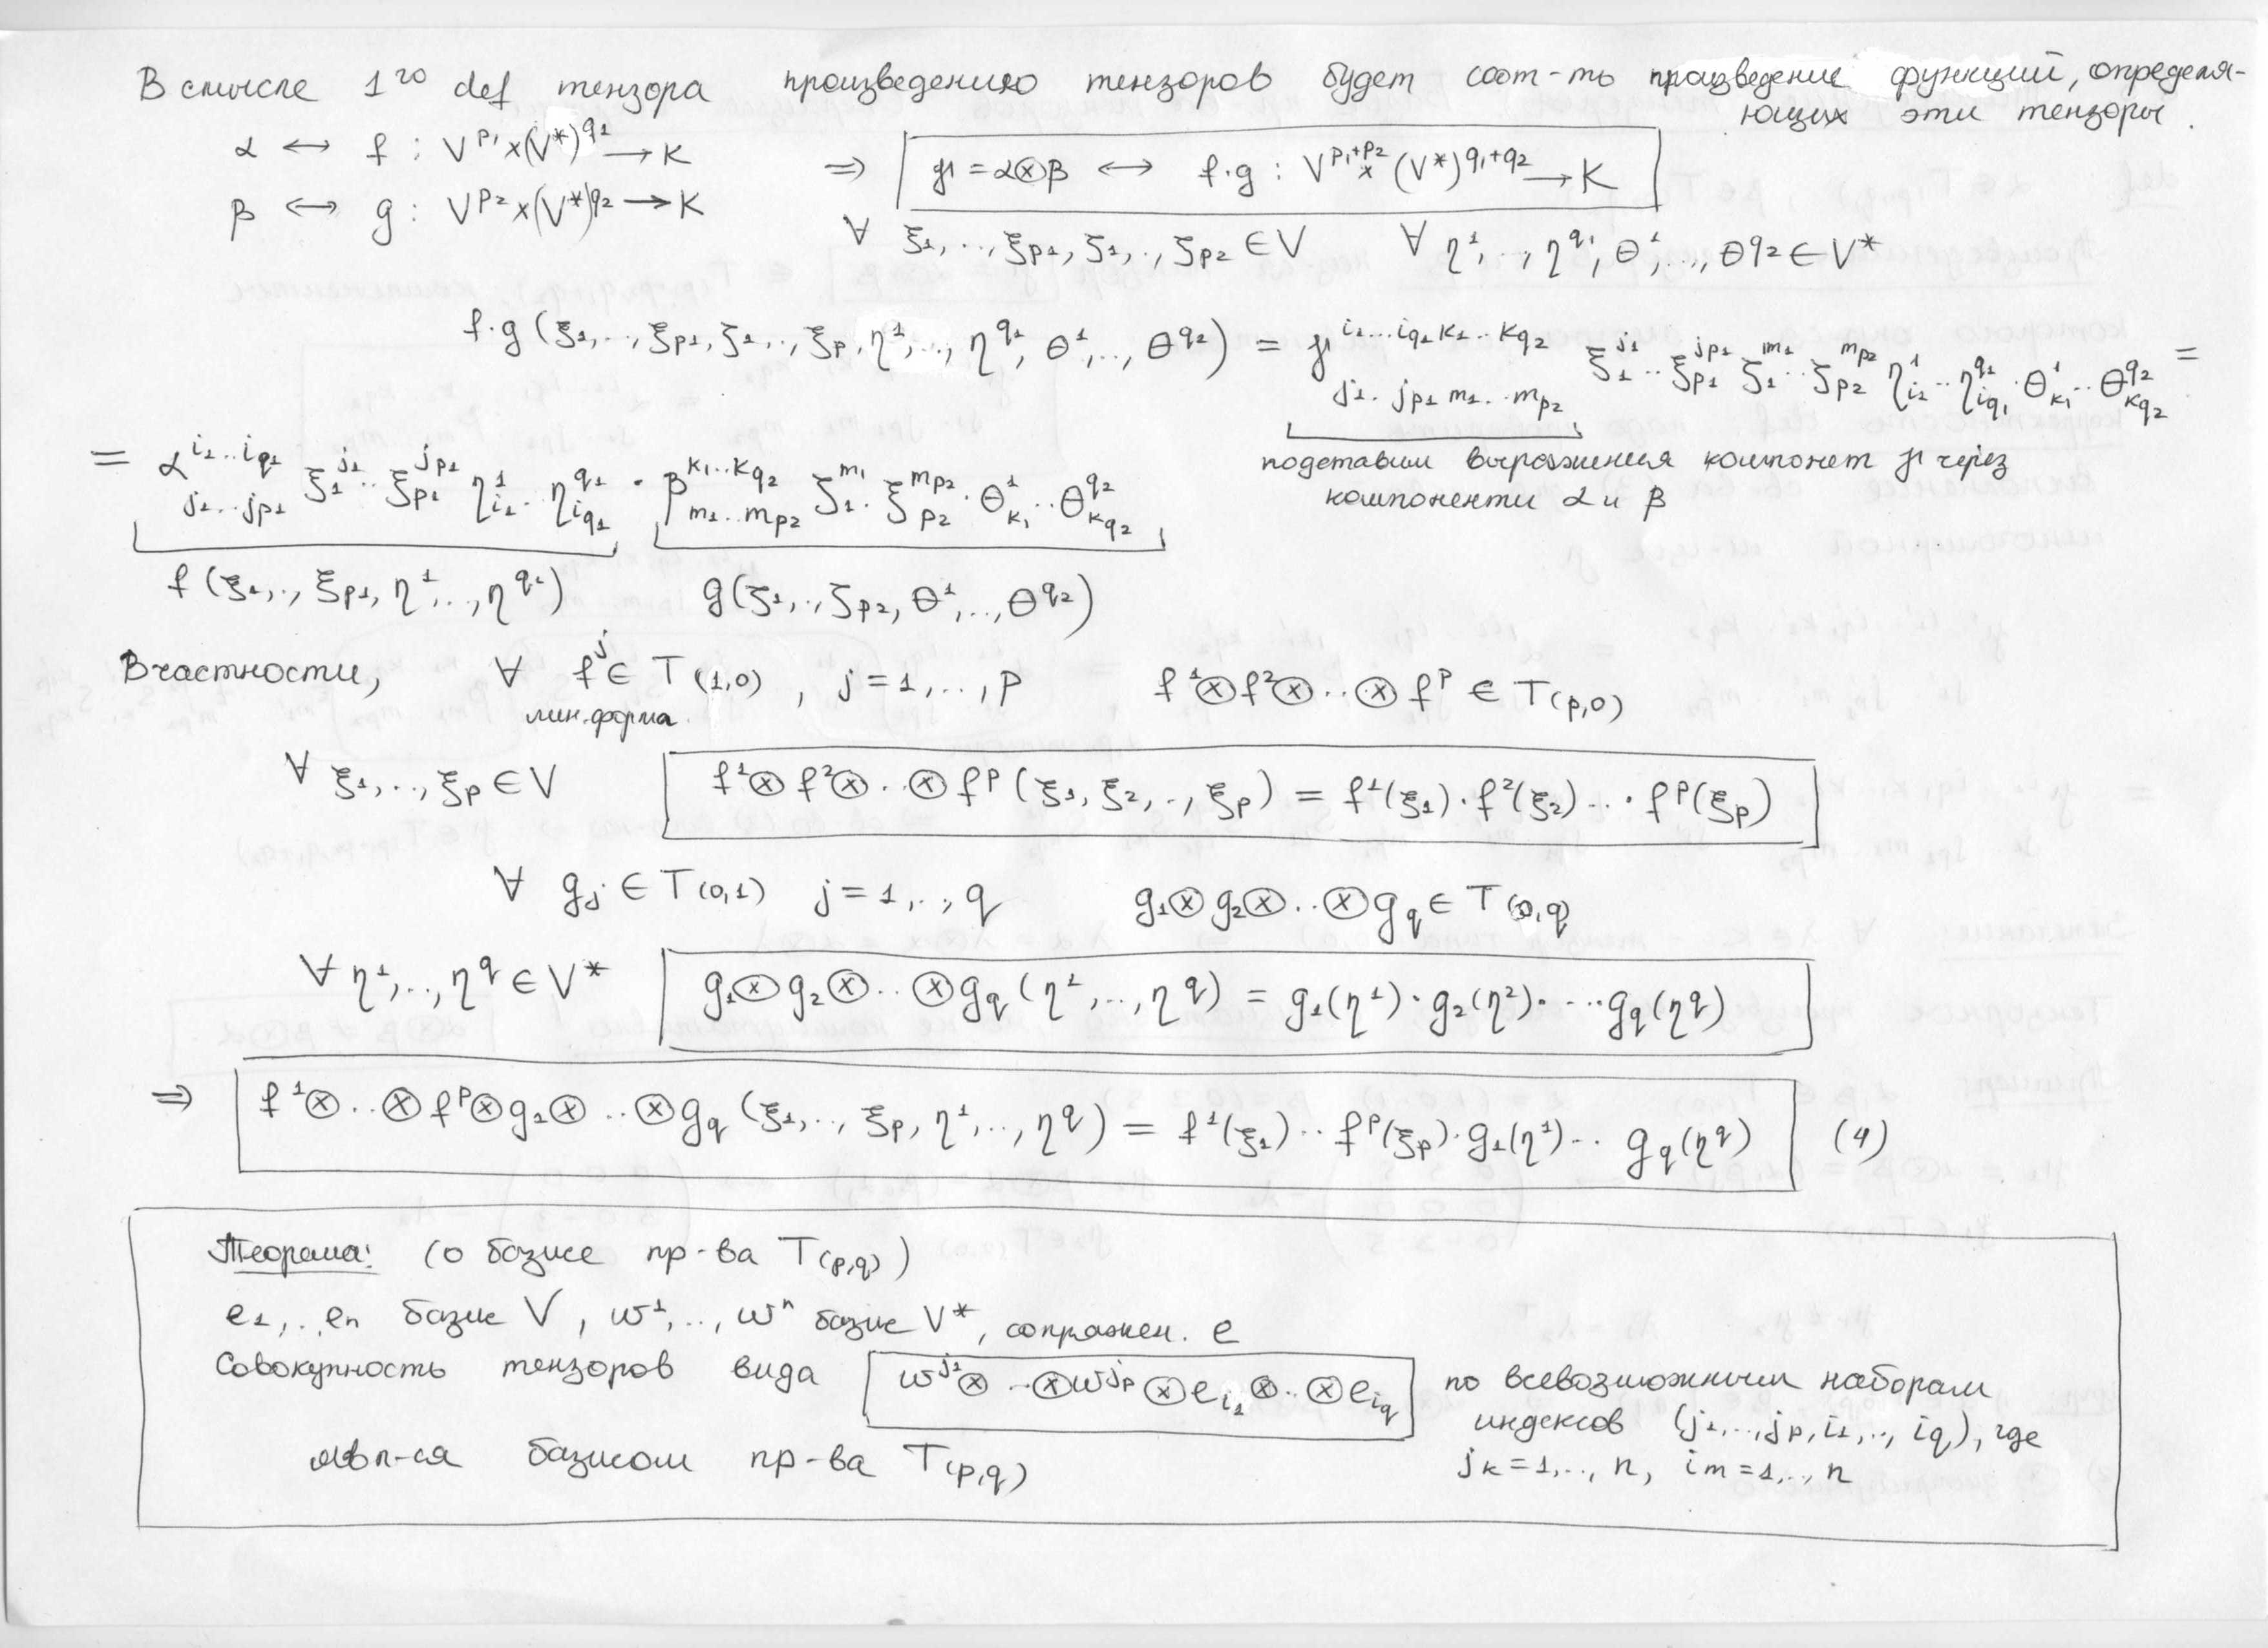
\includegraphics[height=0.49\textheight, width=\textwidth]{03002}	
		\n
		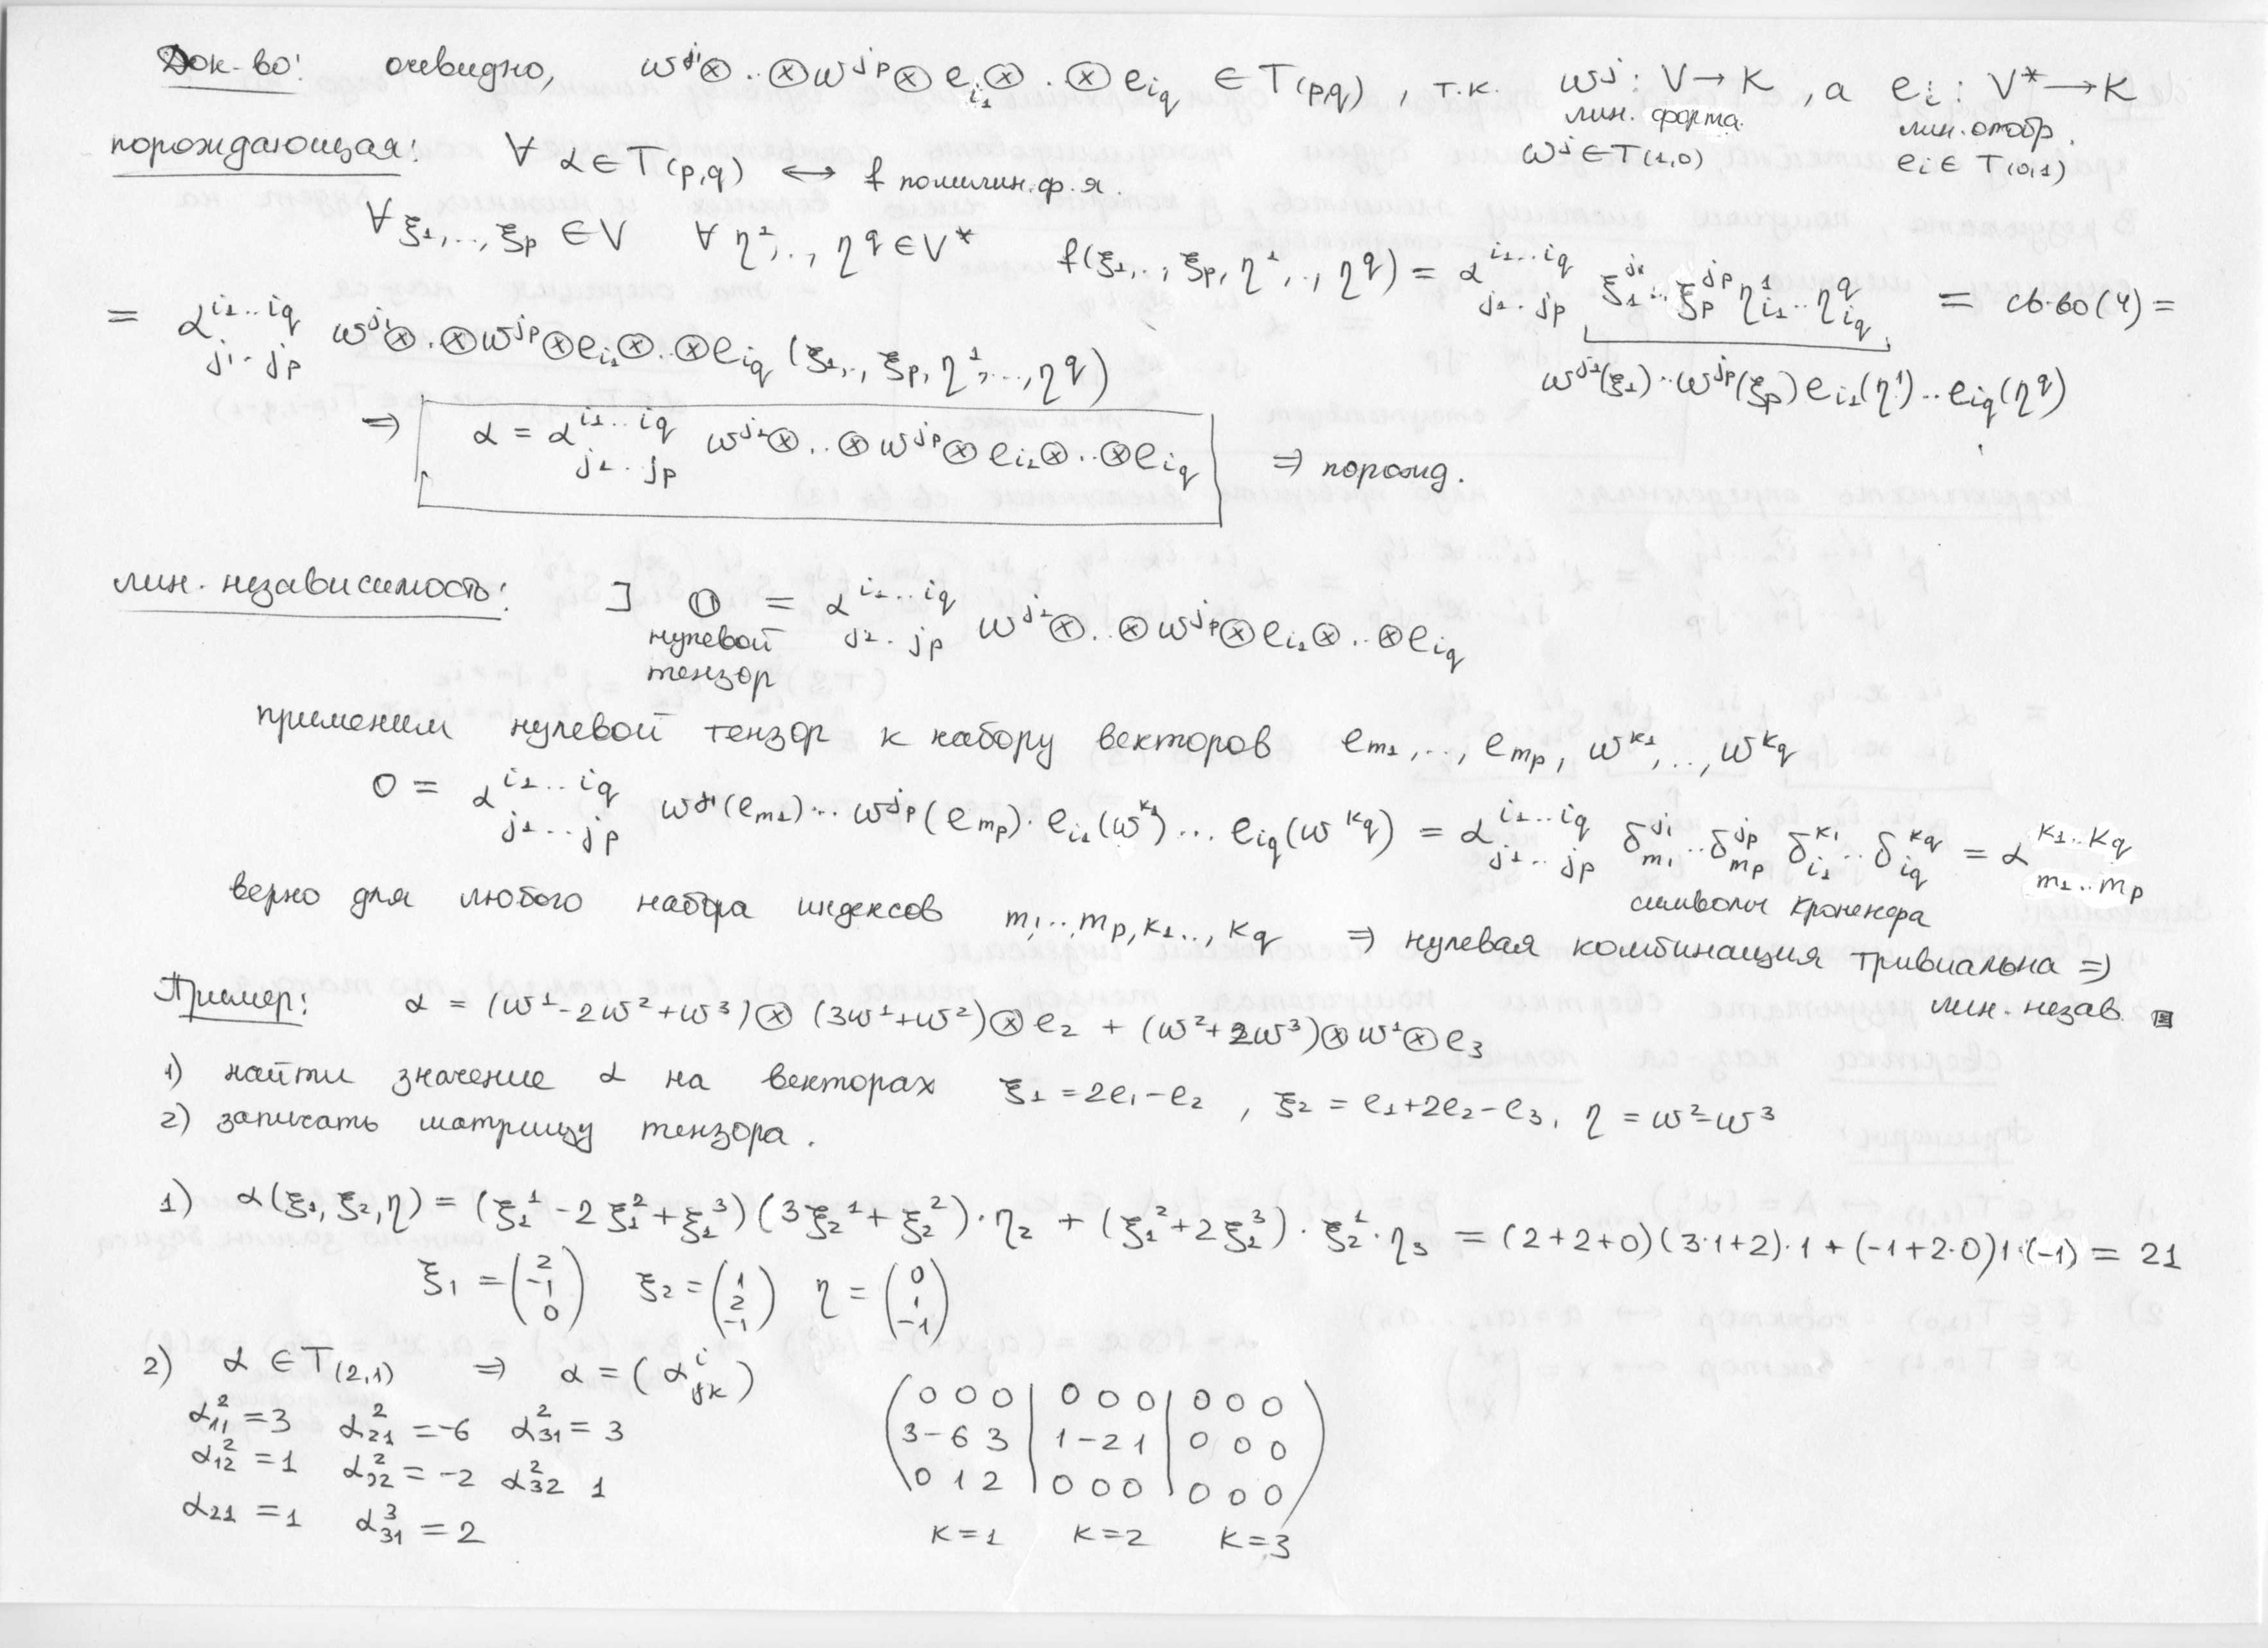
\includegraphics[height=0.49\textheight, width=\textwidth]{03003}		
		\n
		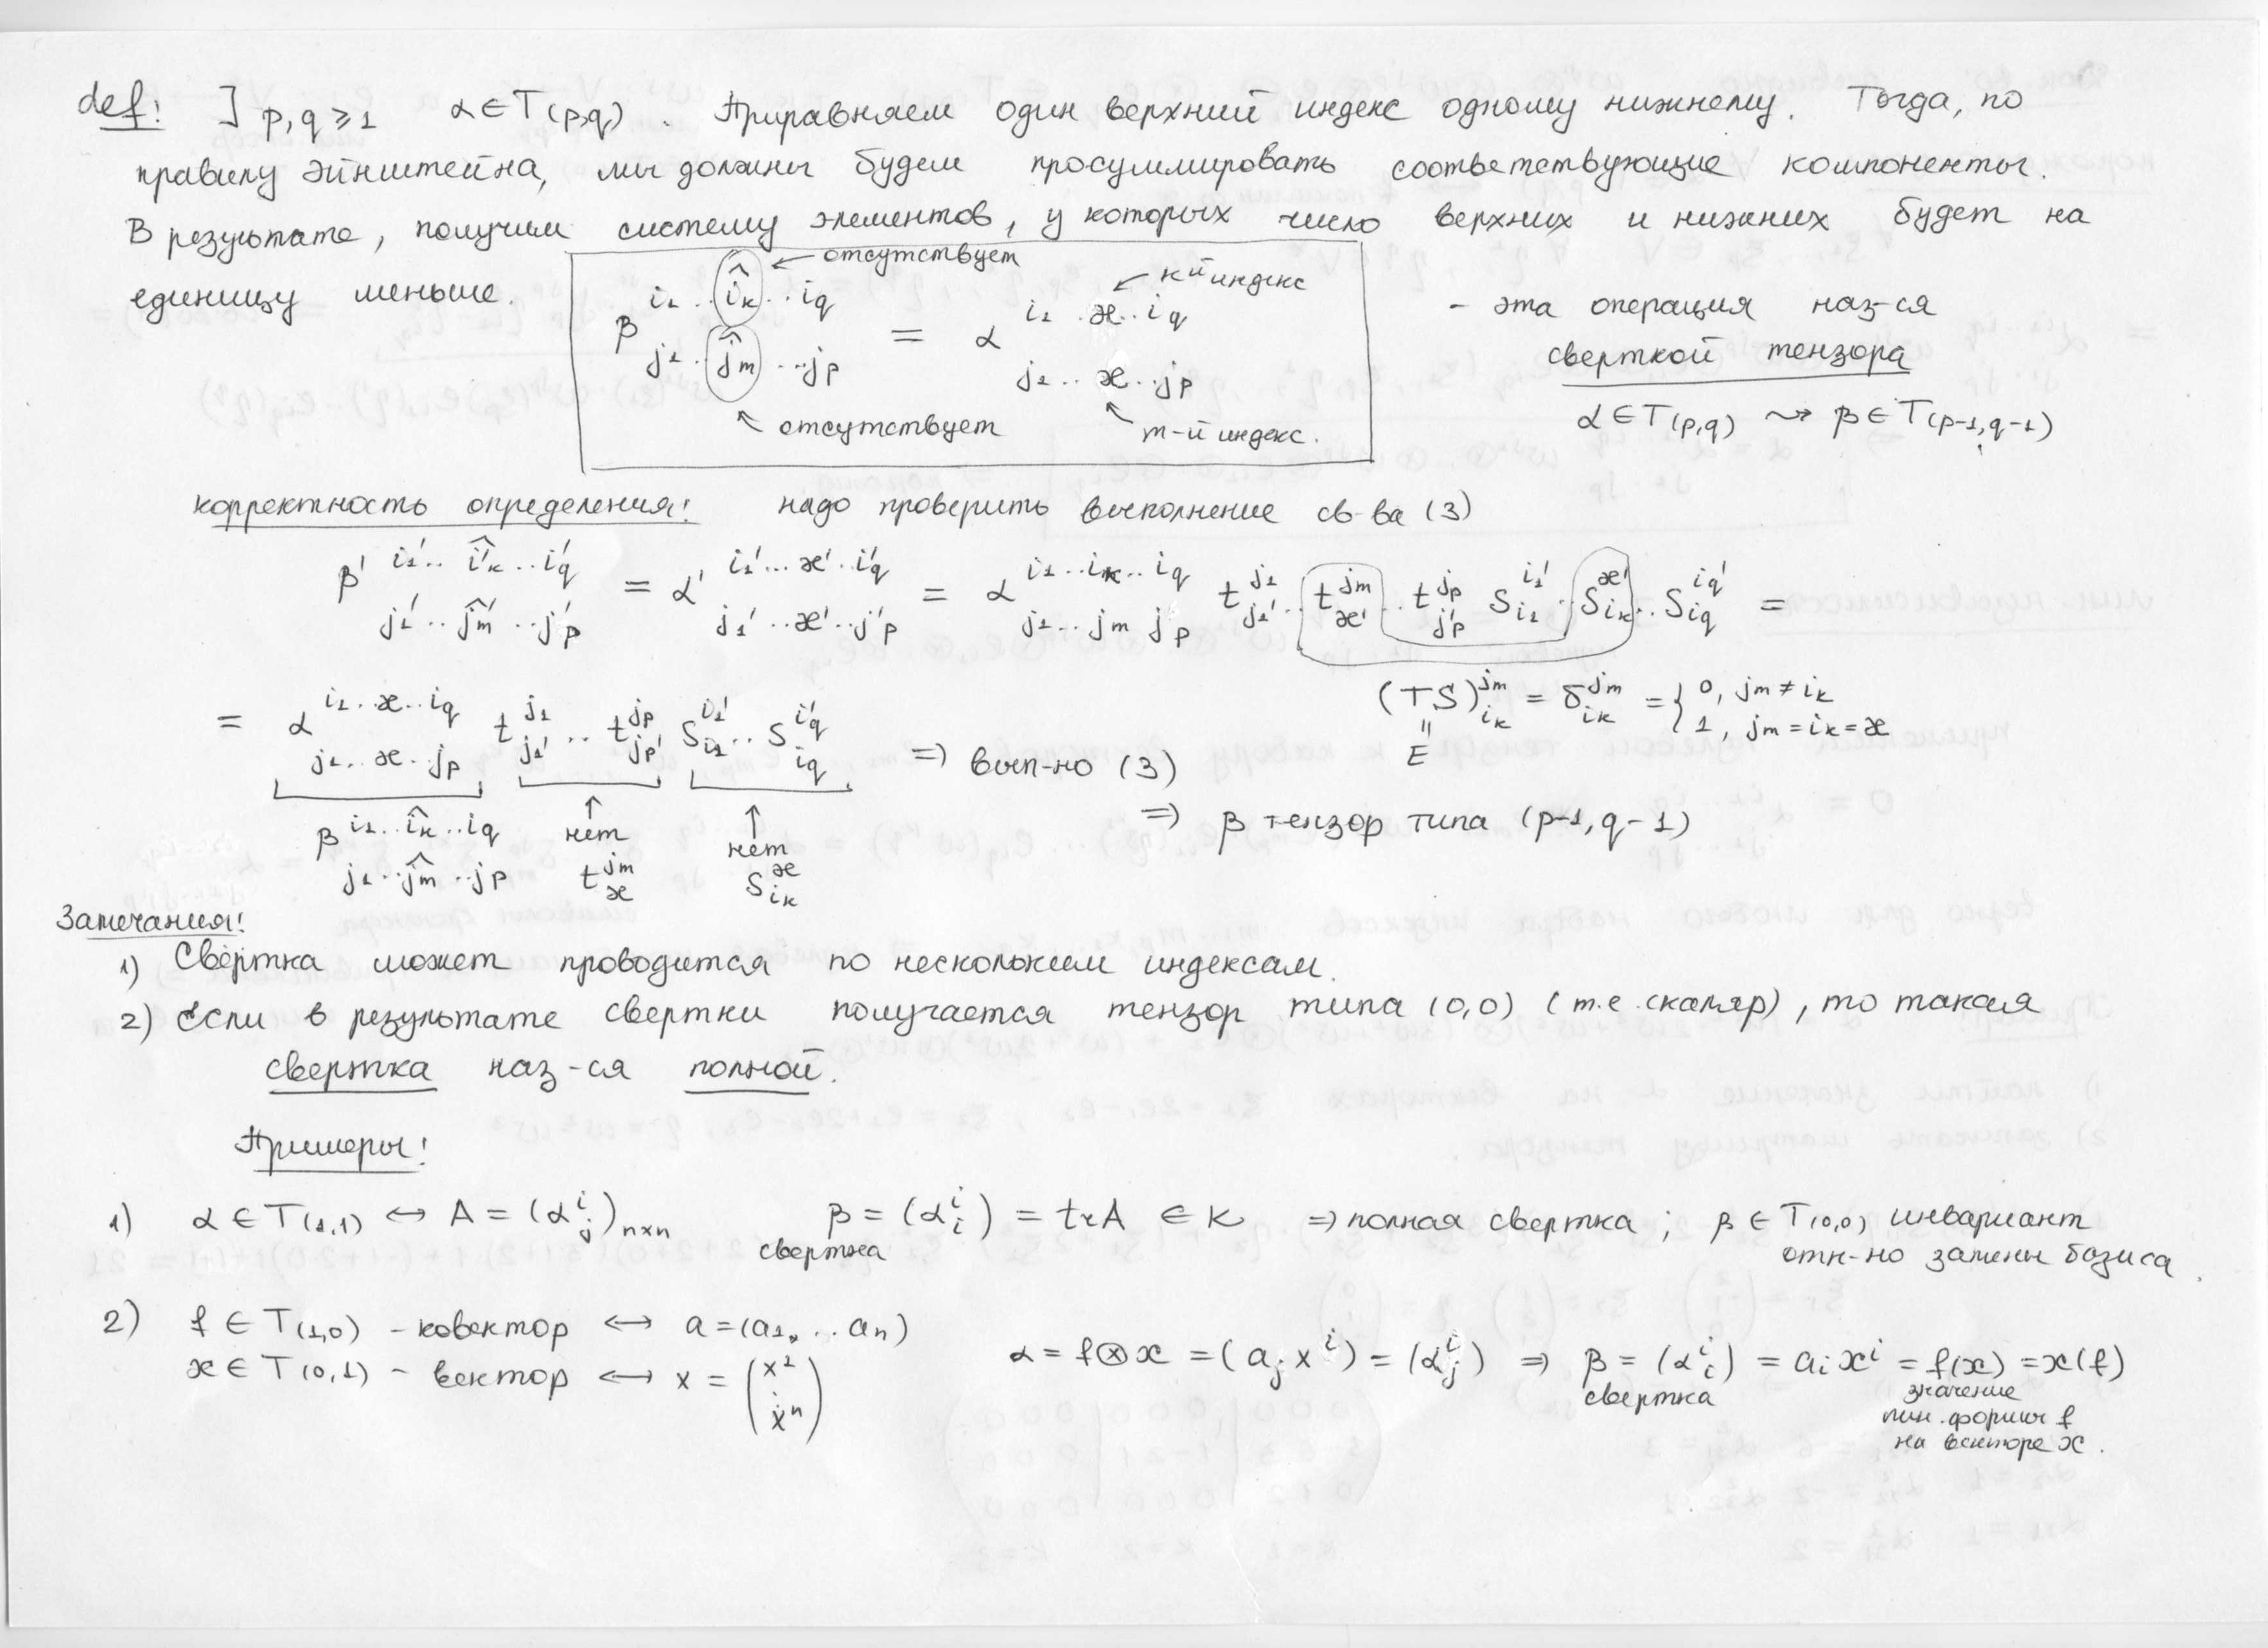
\includegraphics[height=0.49\textheight, width=\textwidth]{03004}	
		\n
		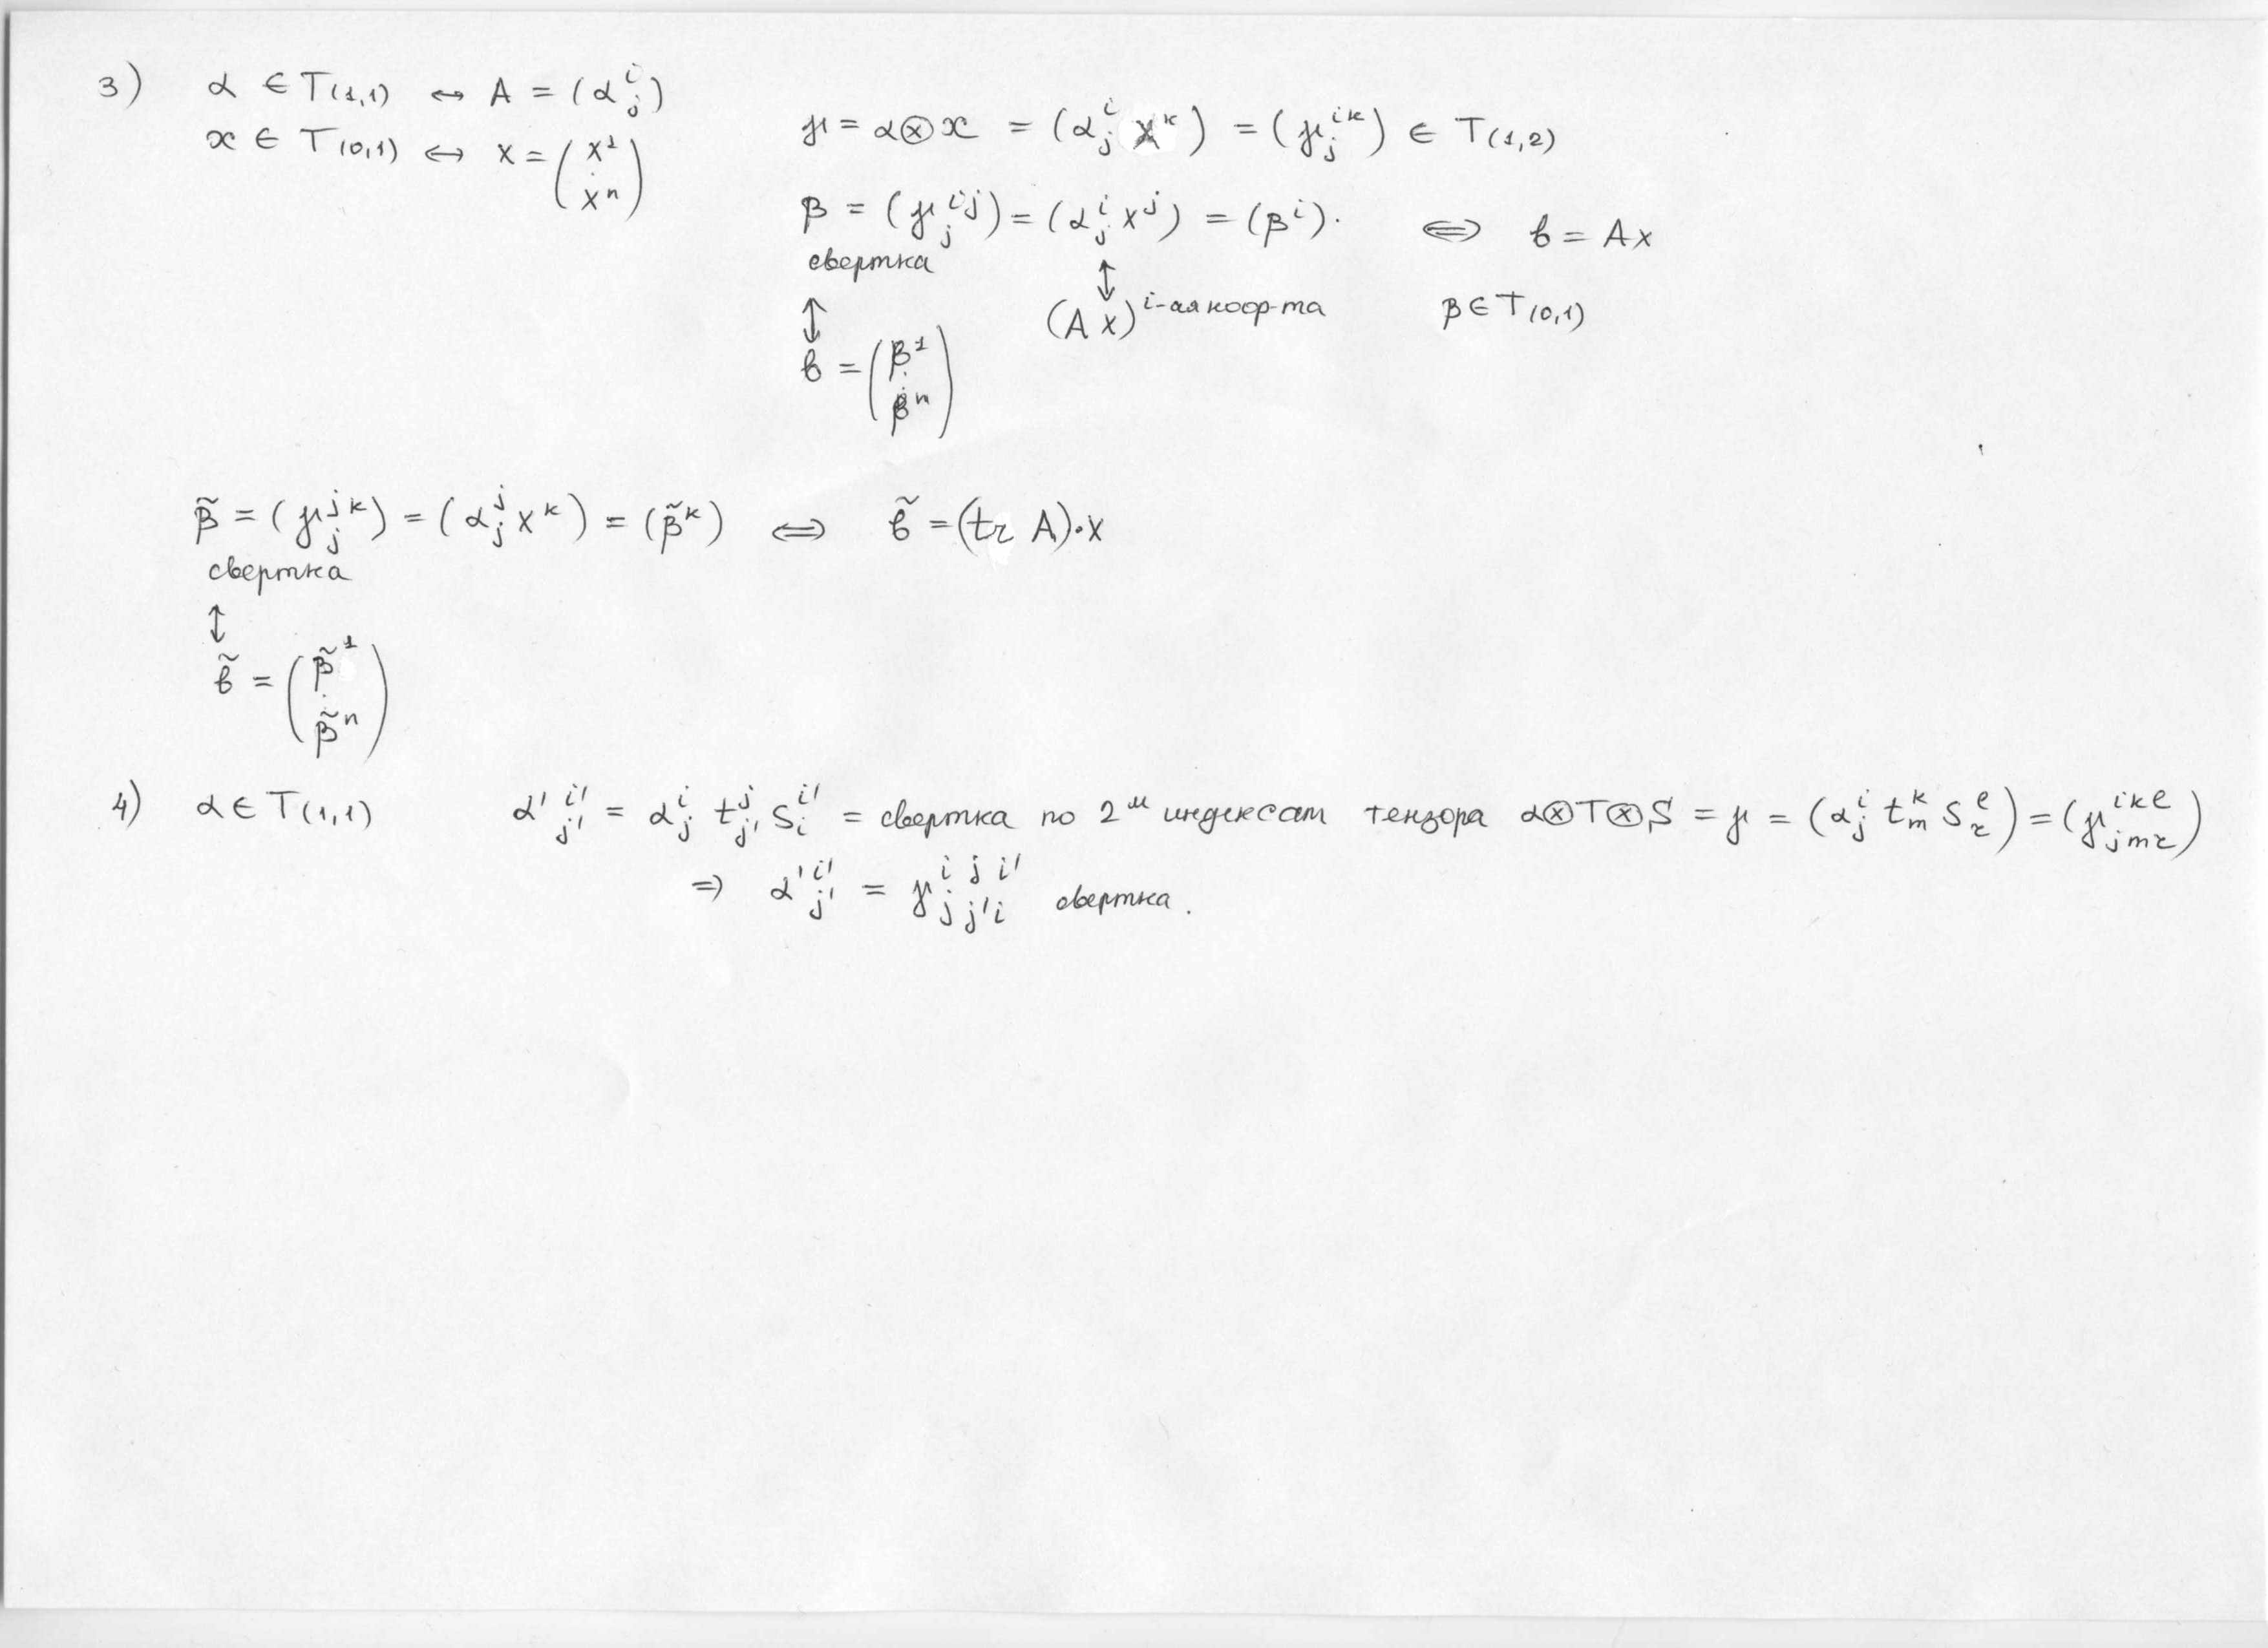
\includegraphics[height=0.49\textheight, width=\textwidth]{03005}	
		\n			
		
		
	\subsection{Транспонирование тензора. Симметрические и кососимметричческие тензоры.}
	 	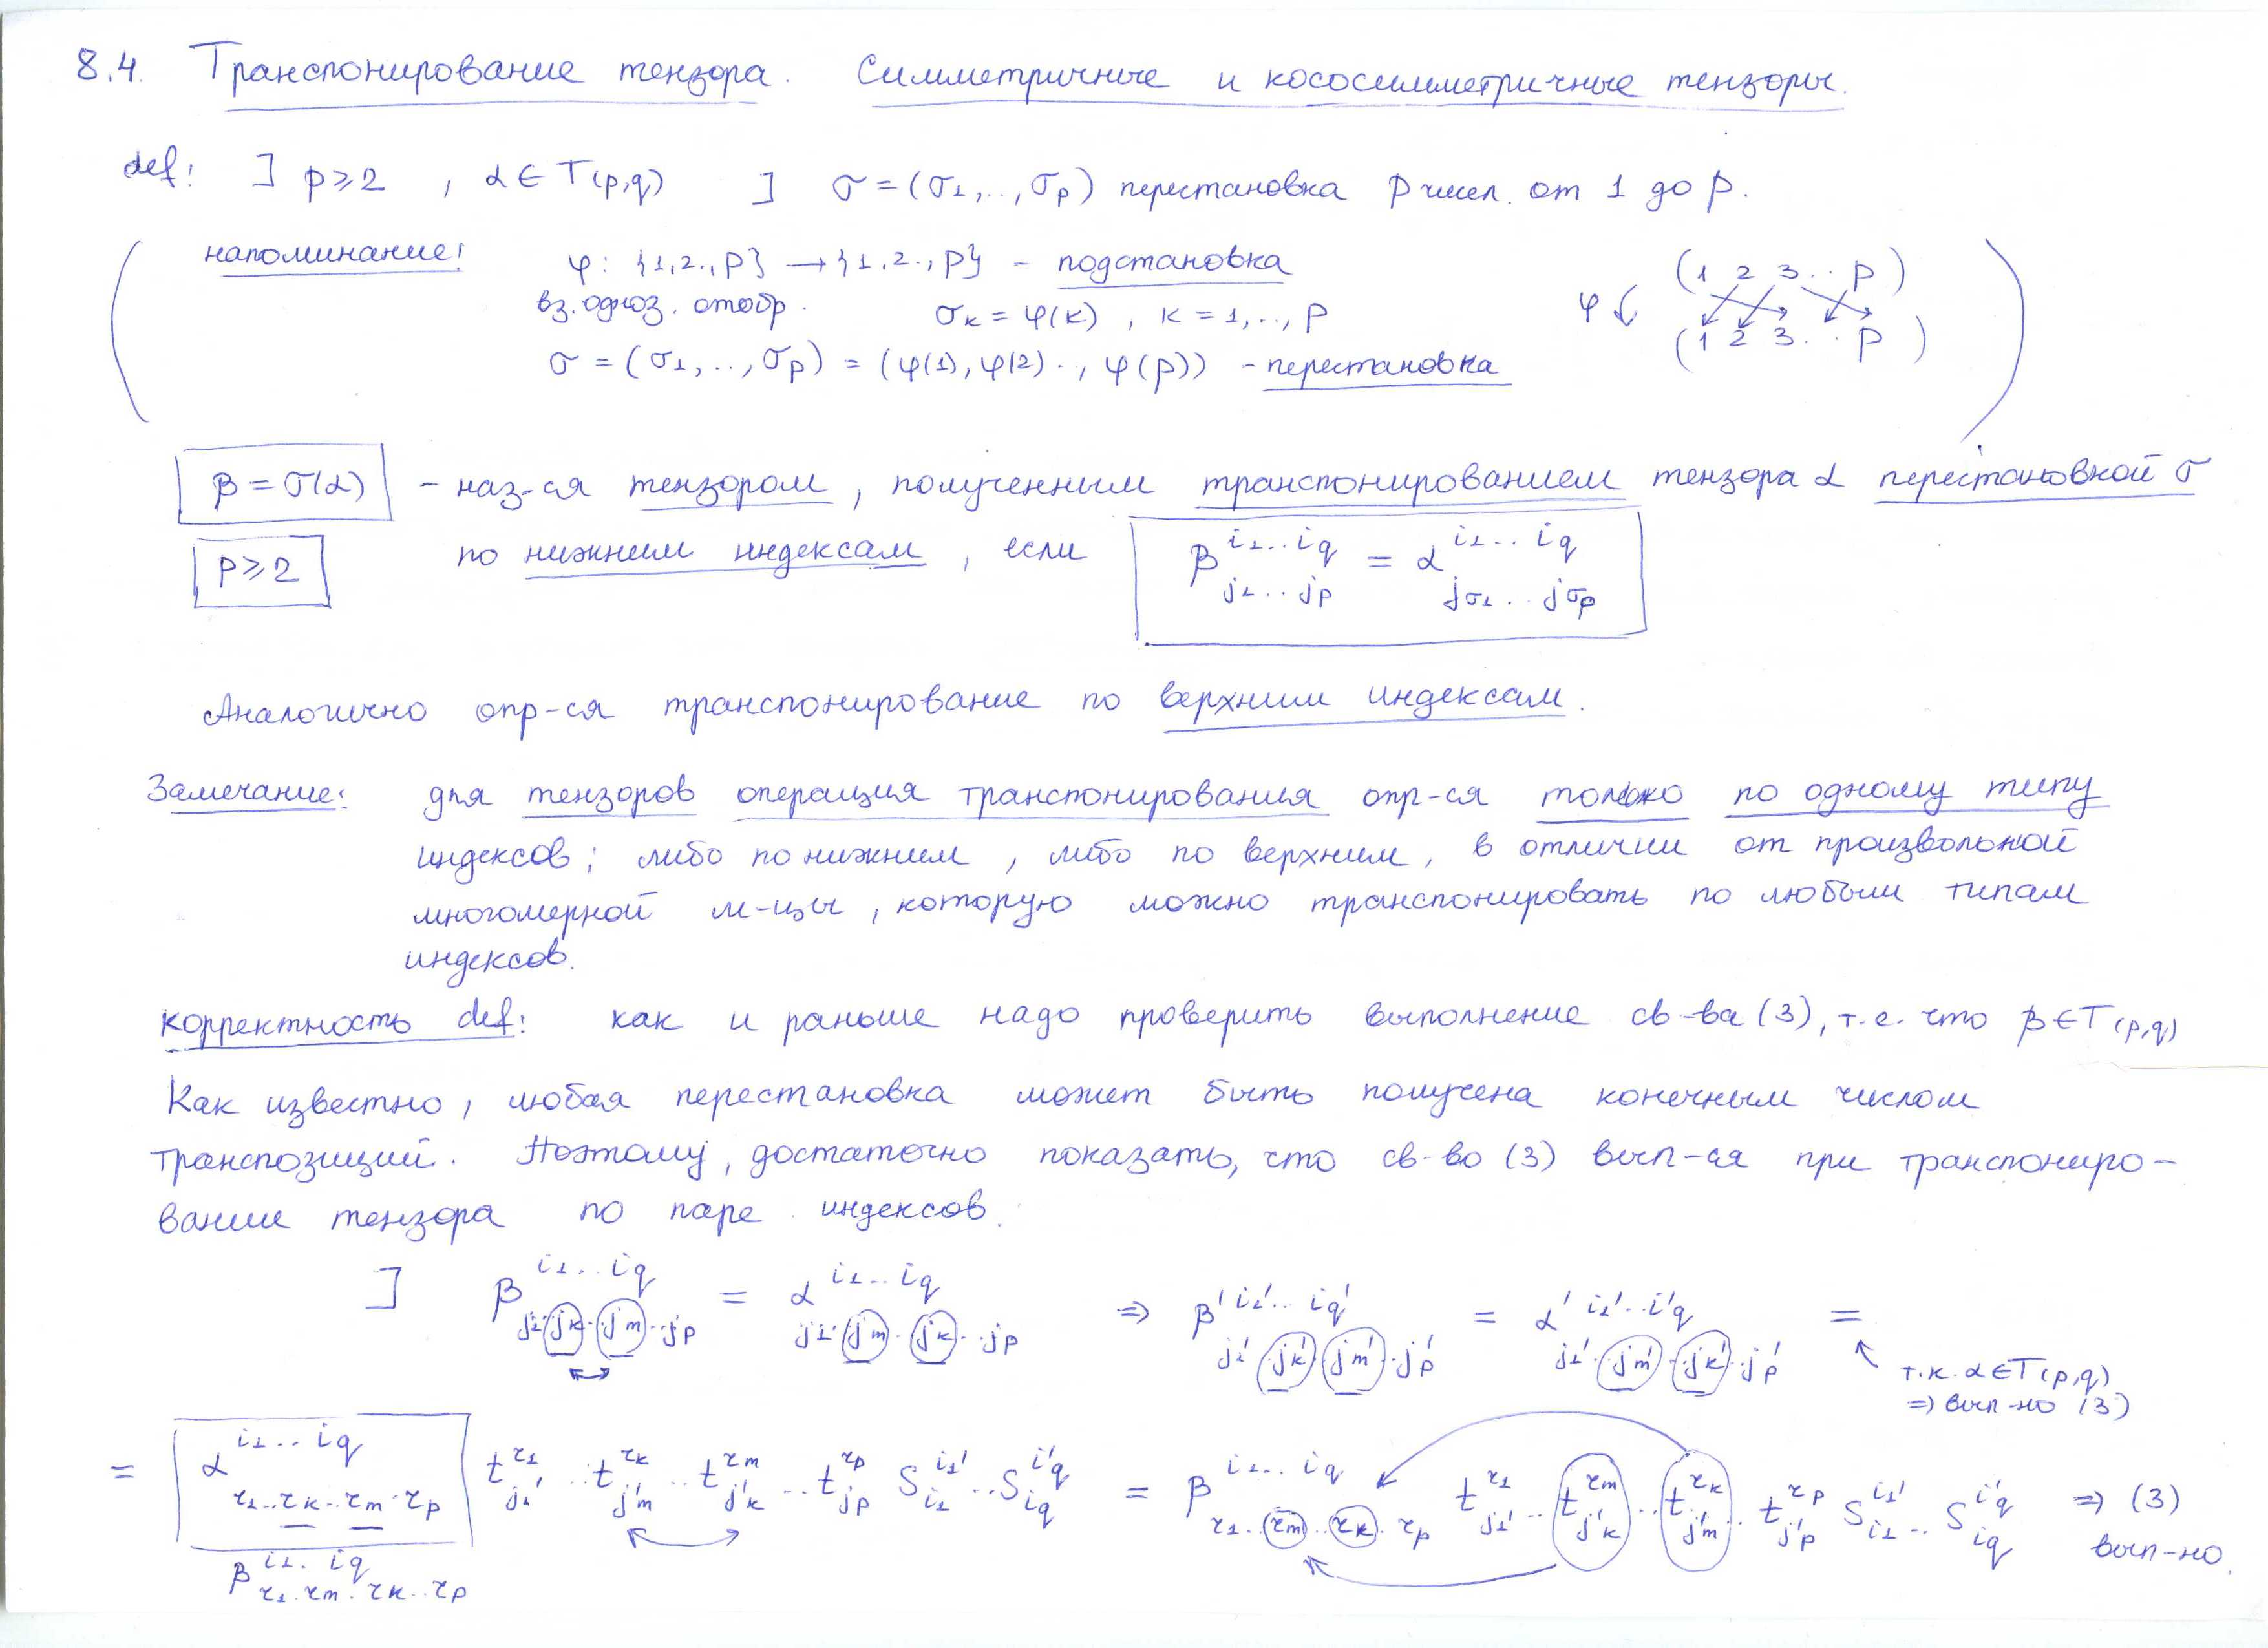
\includegraphics[height=0.49\textheight, width=\textwidth]{04001}	
		\n
		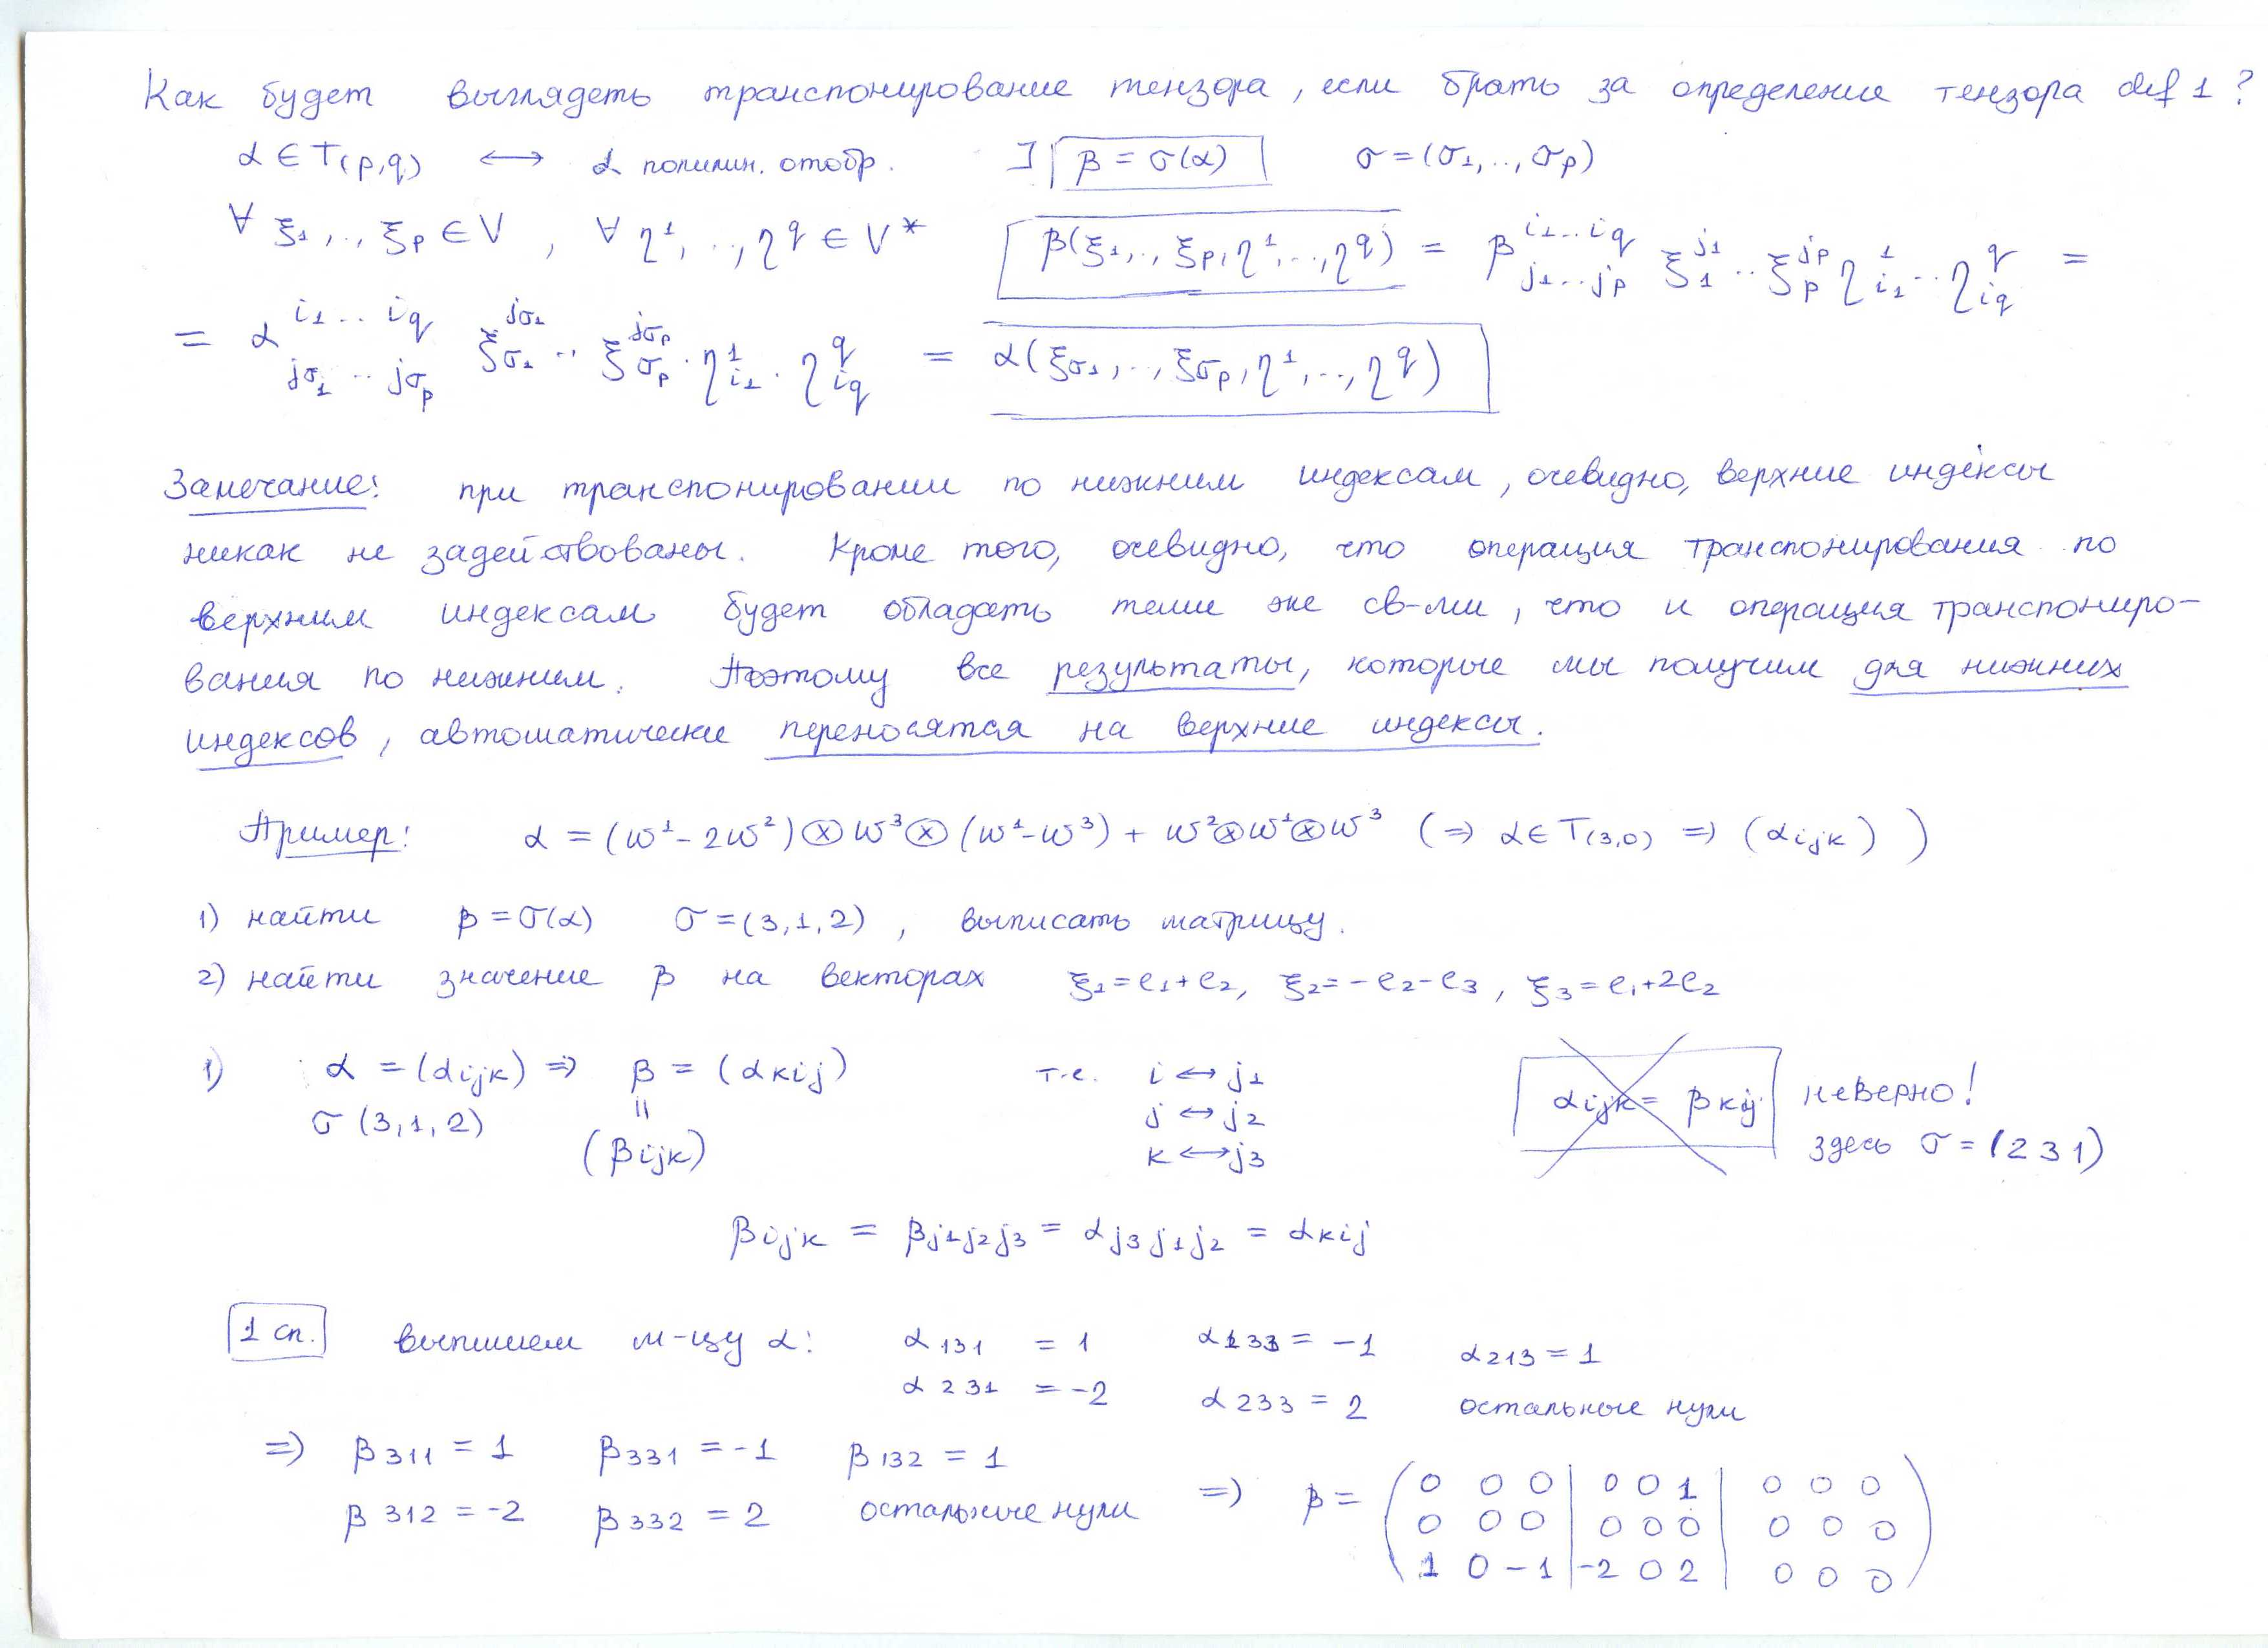
\includegraphics[height=0.49\textheight, width=\textwidth]{04002}	
		\n
		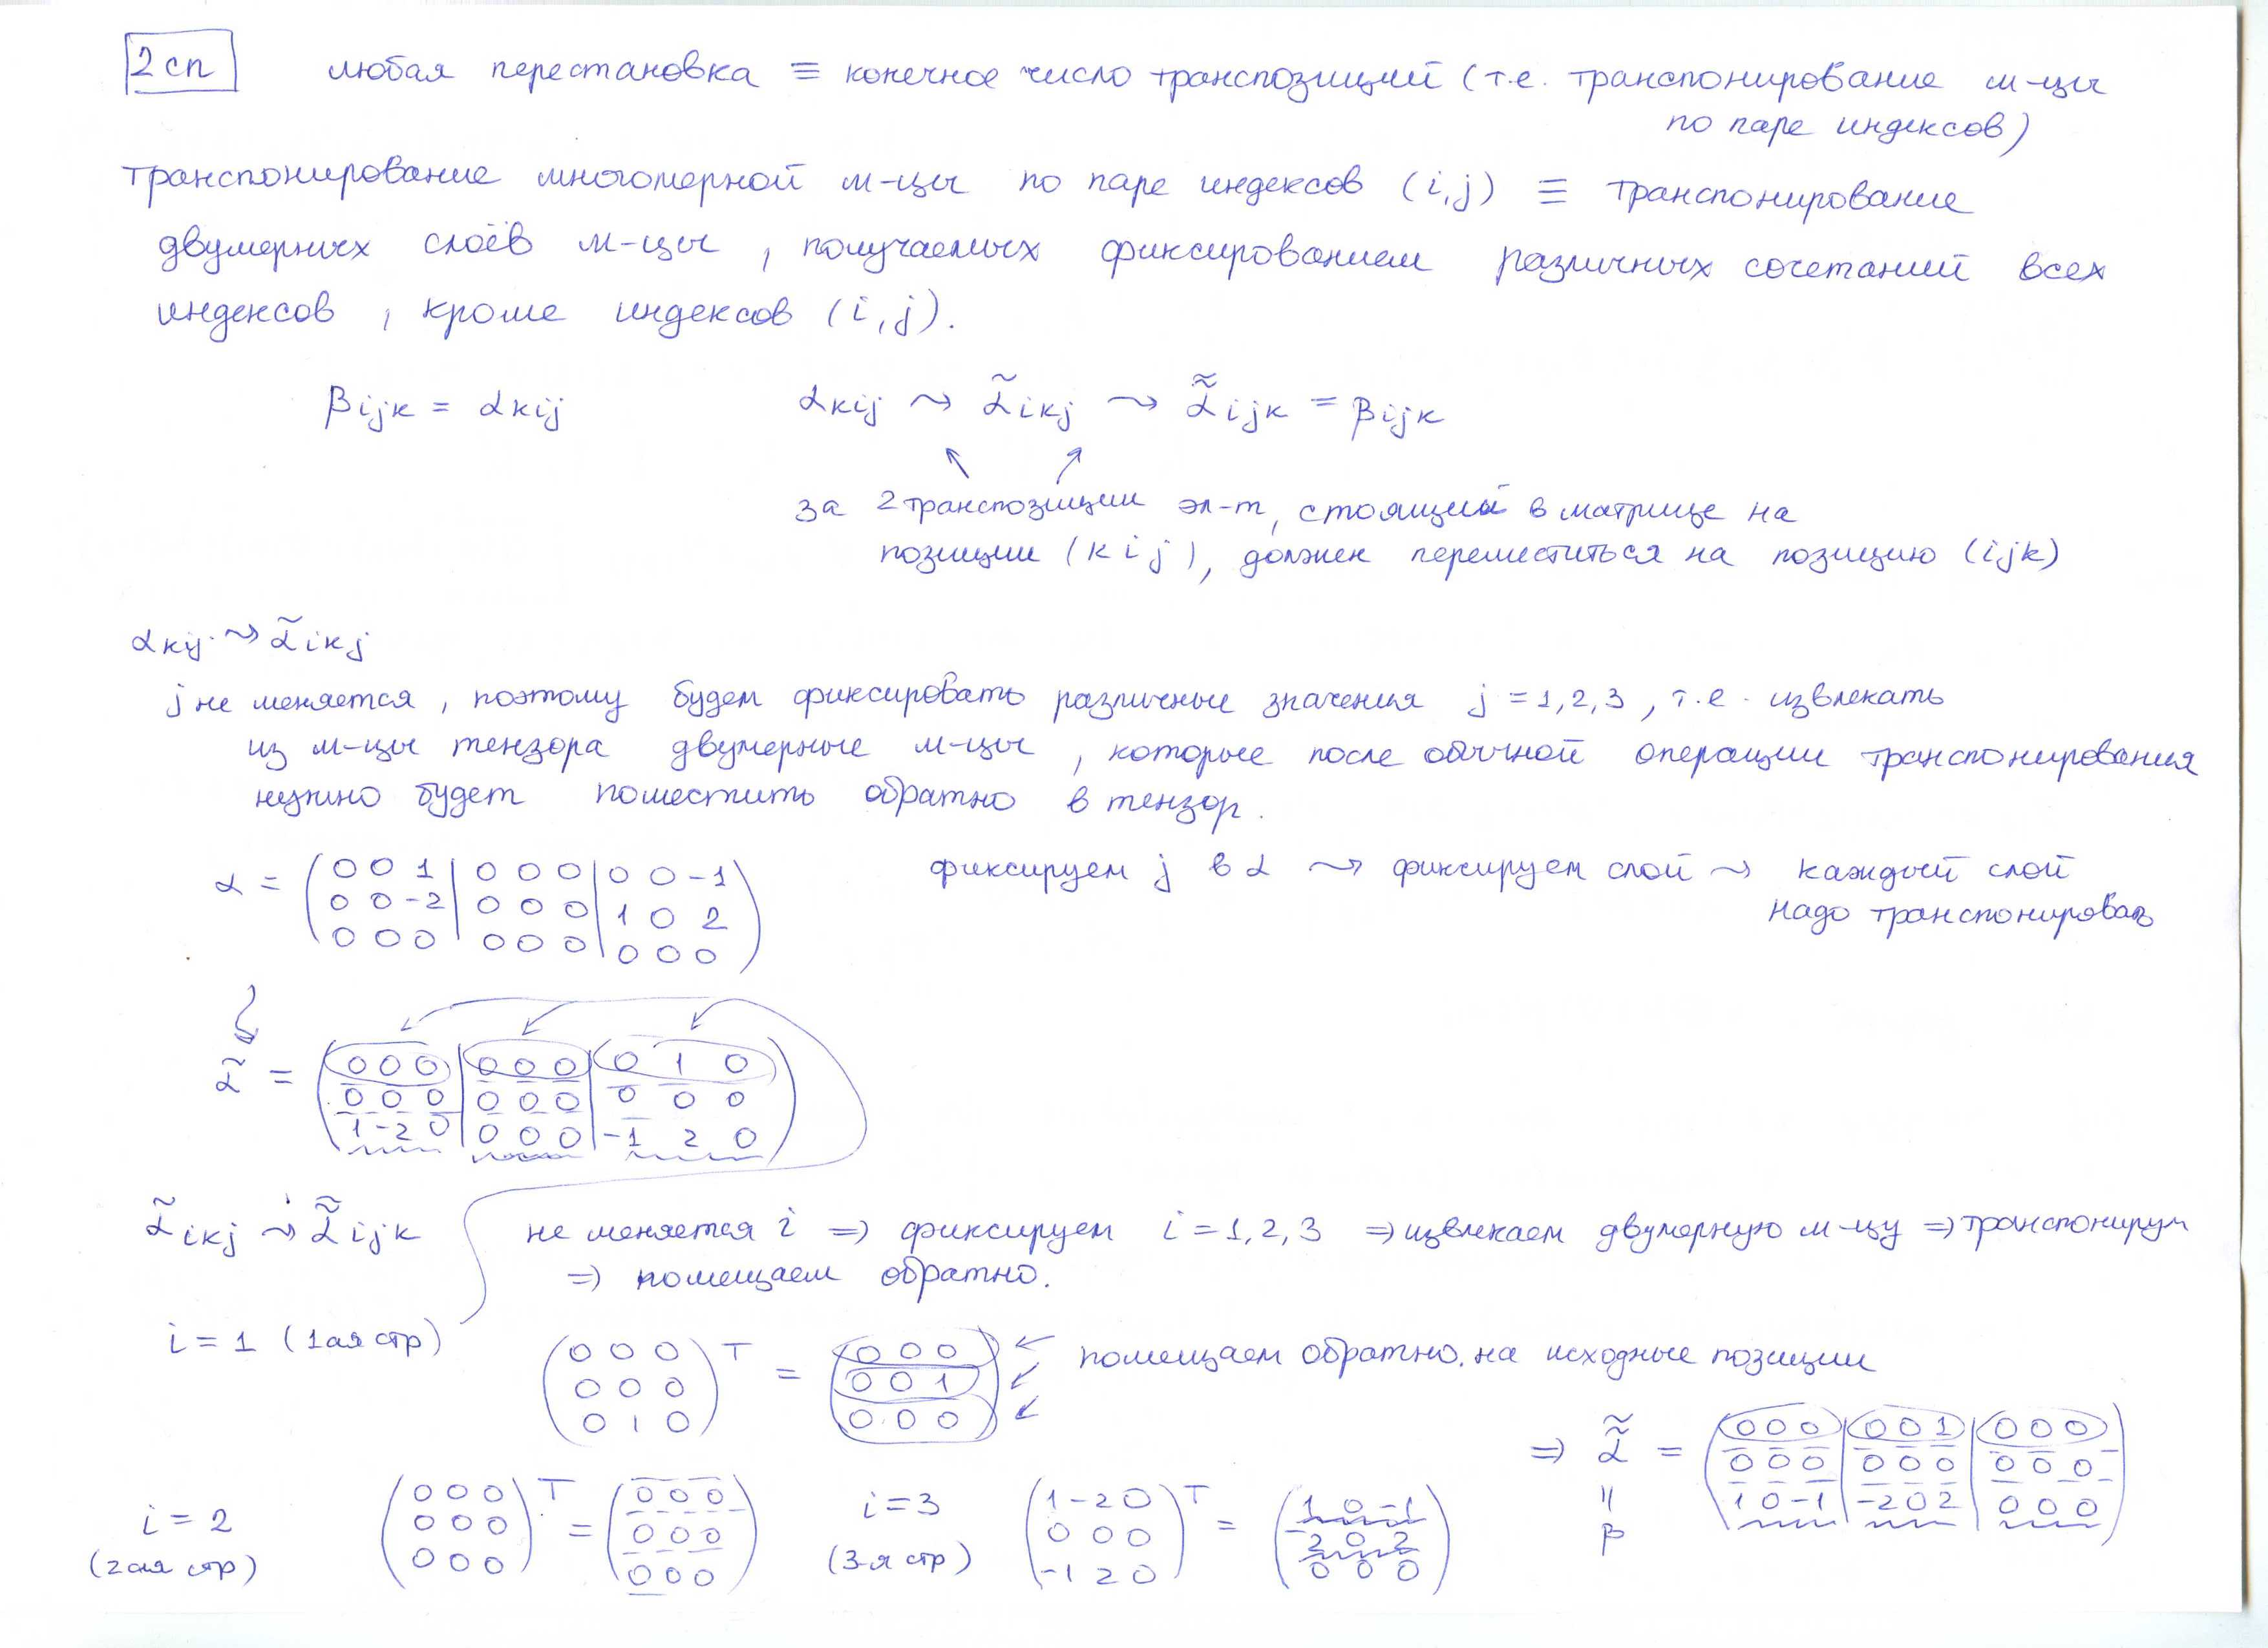
\includegraphics[height=0.49\textheight, width=\textwidth]{04003}	
		\n
		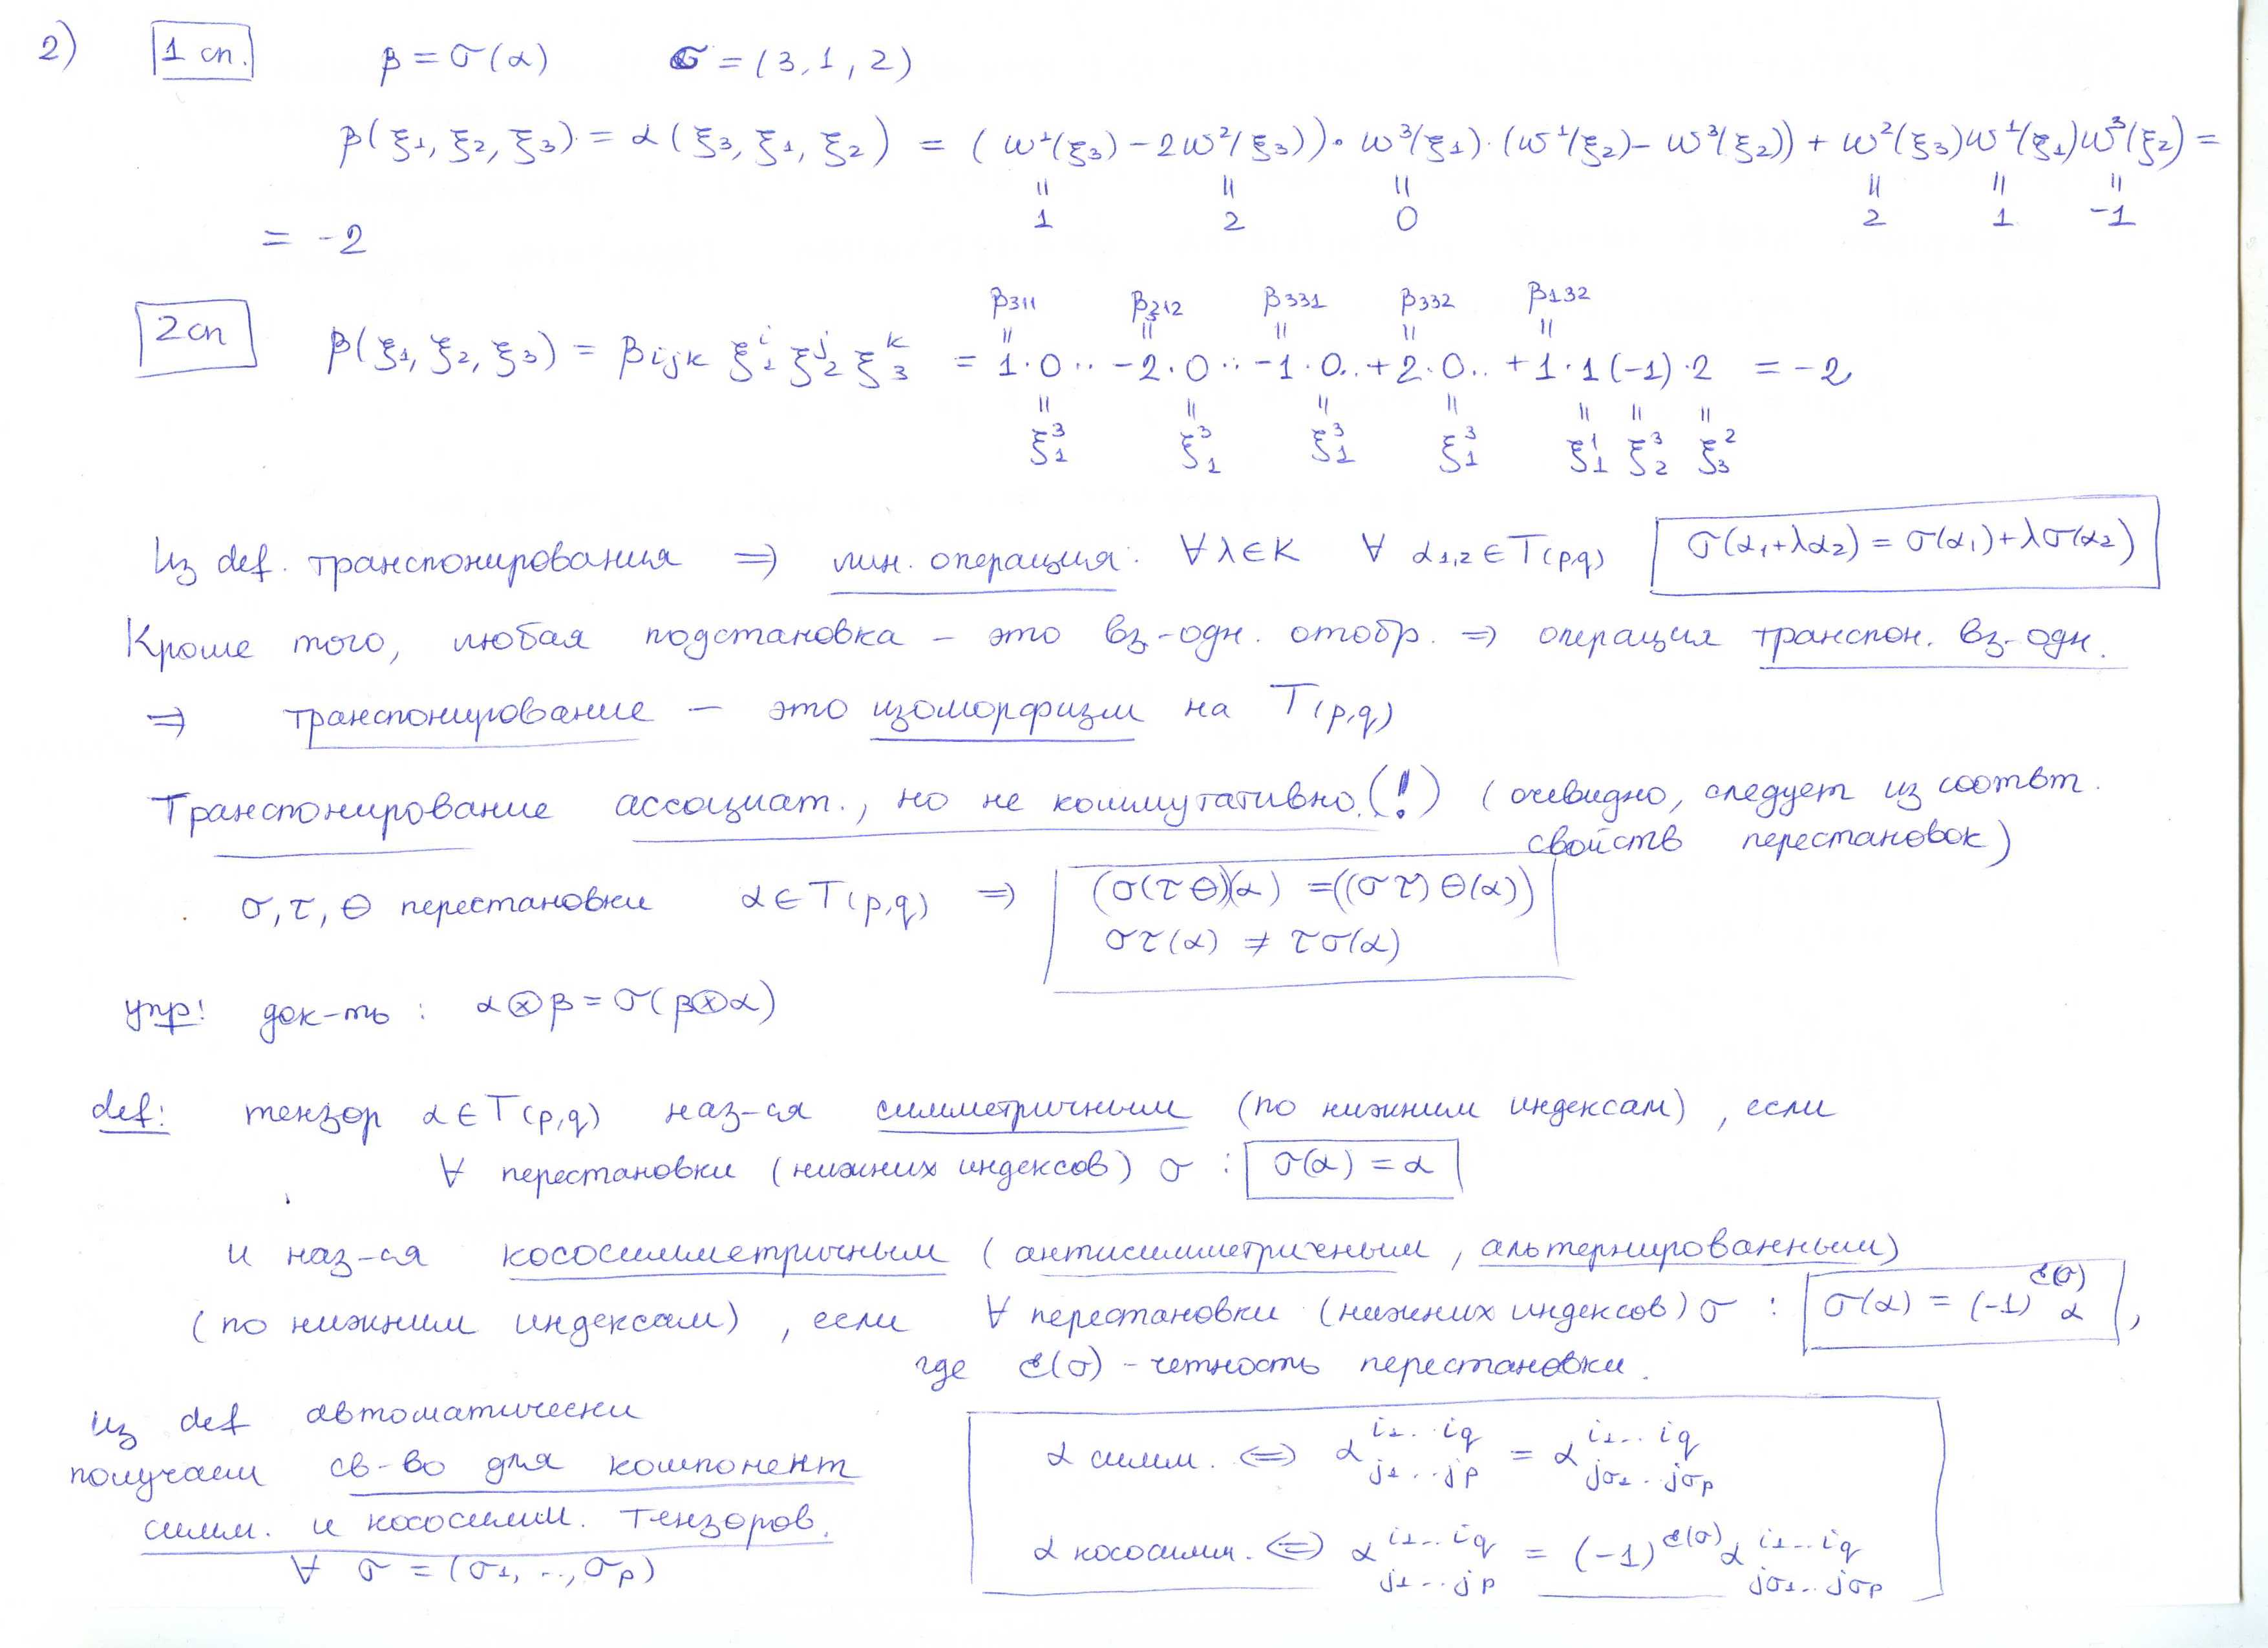
\includegraphics[height=0.49\textheight, width=\textwidth]{04004}	
		\n
		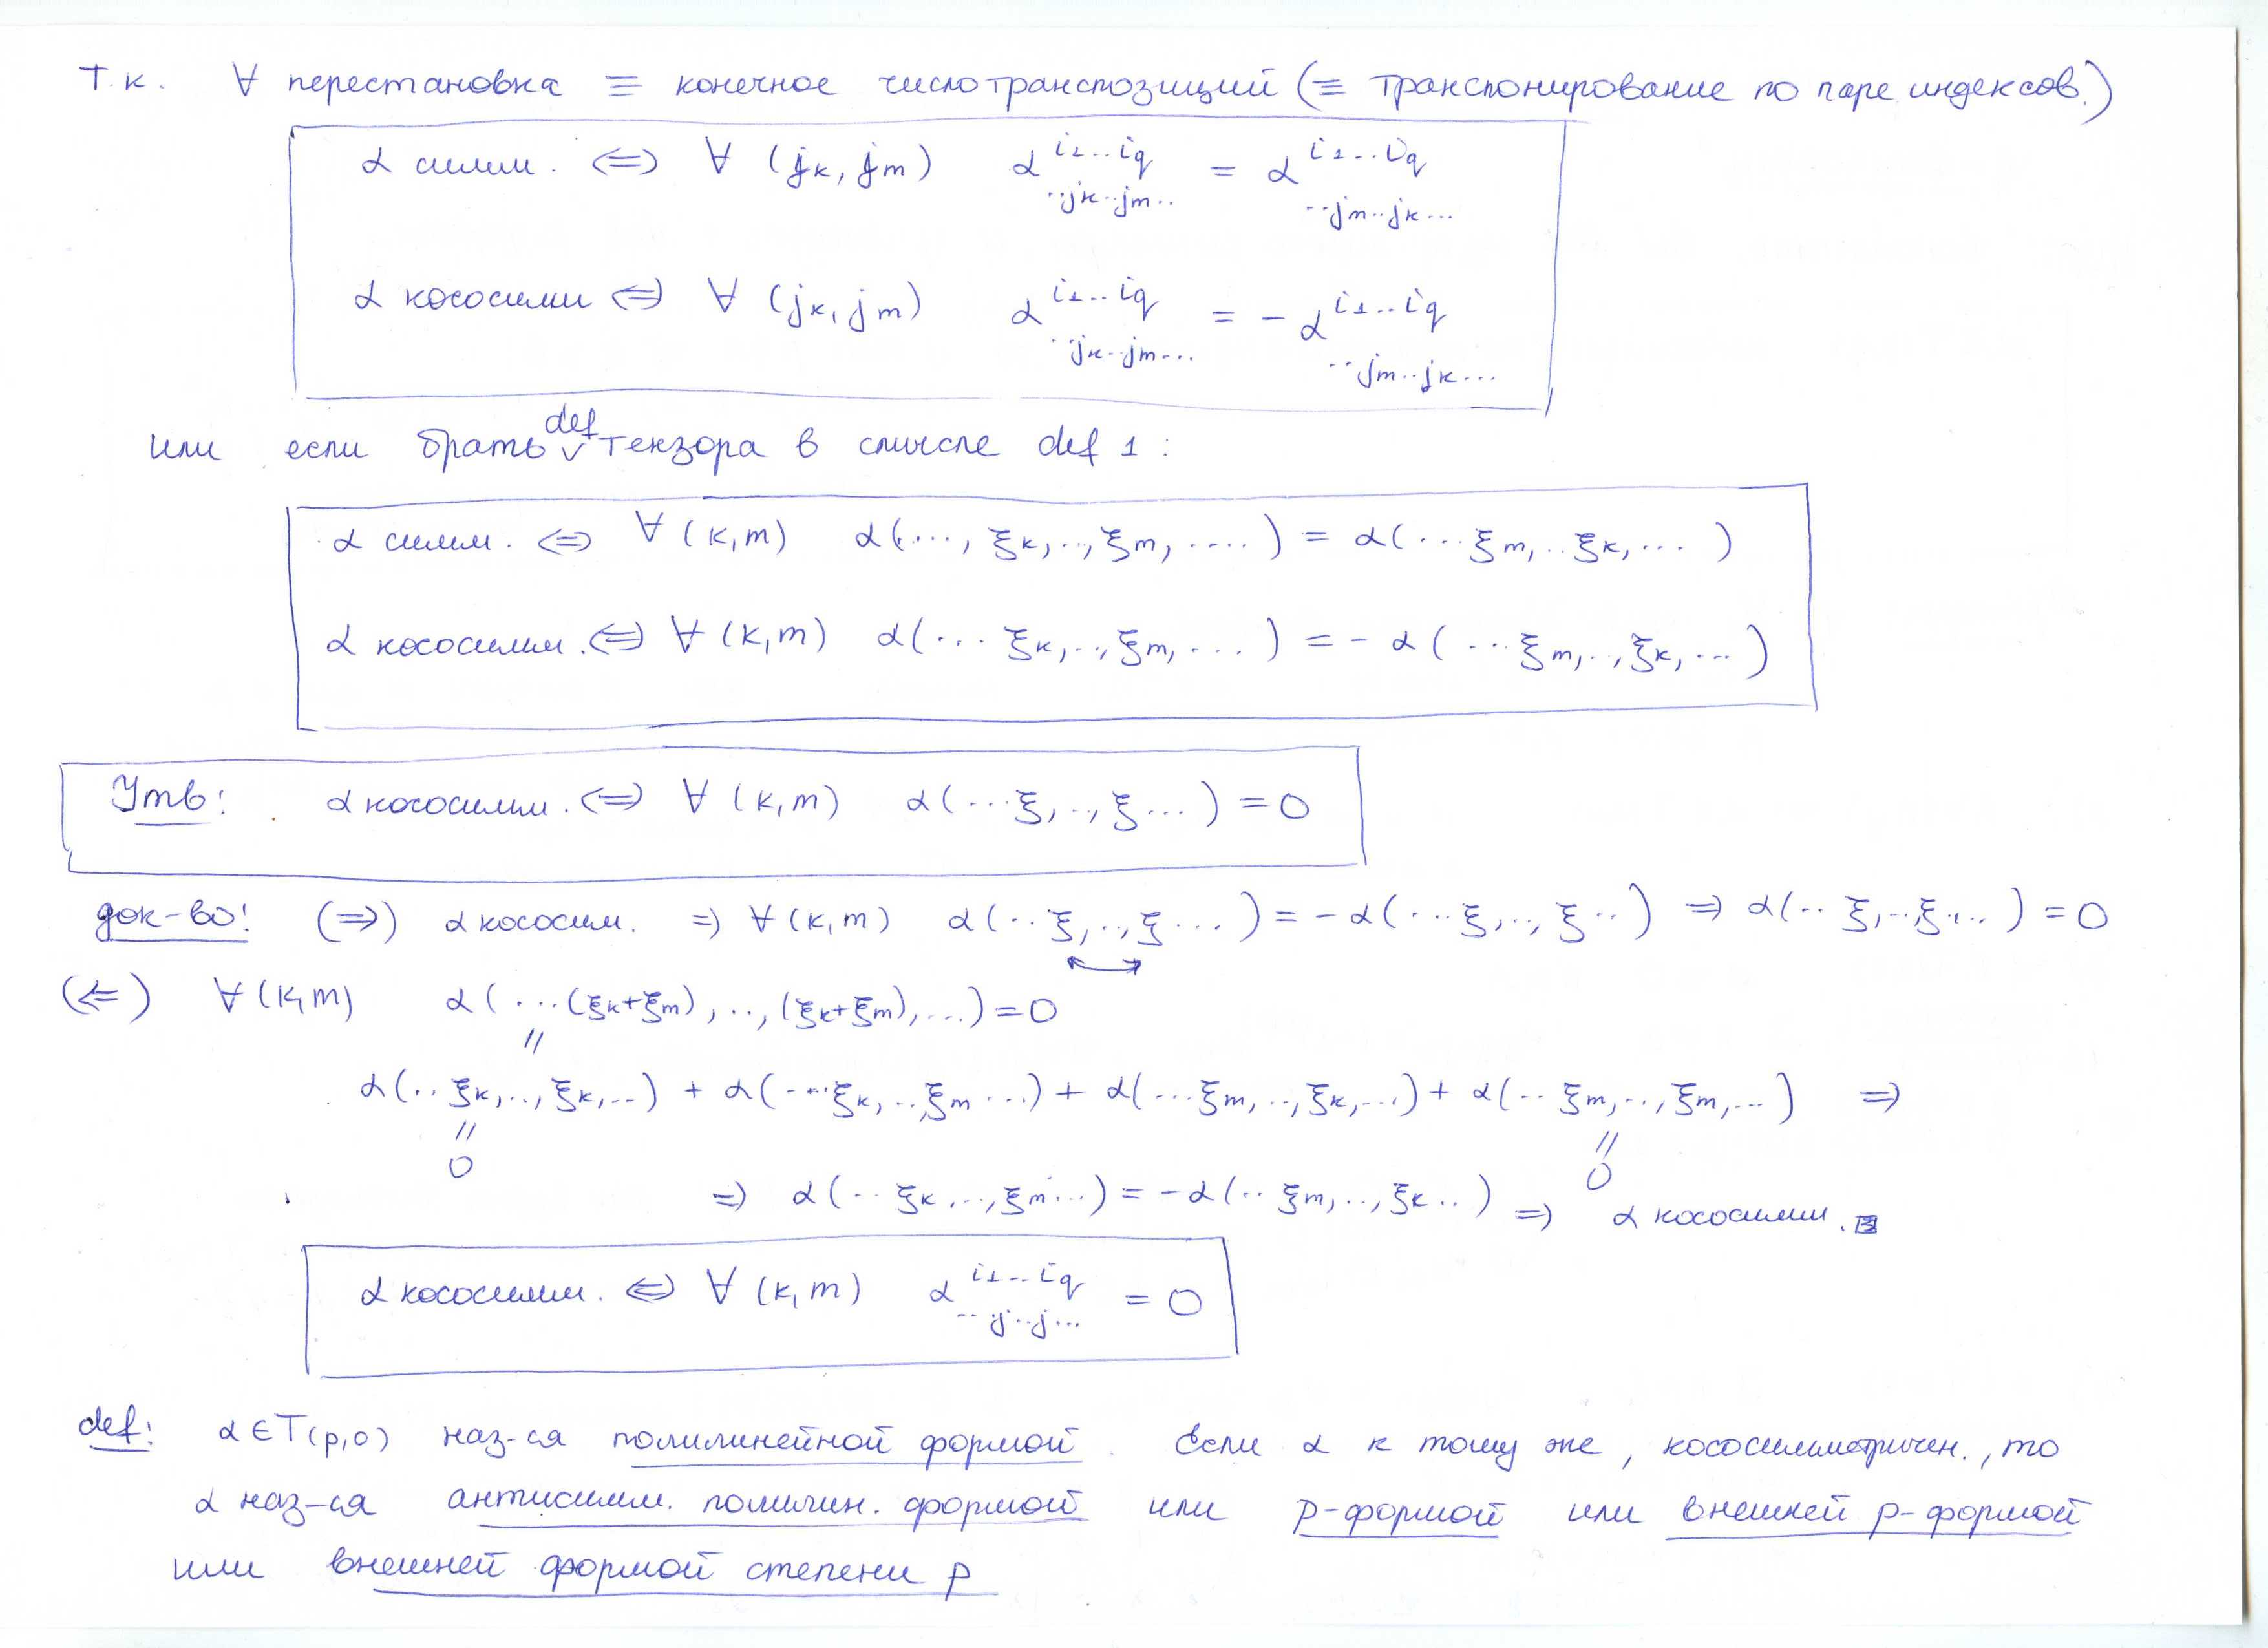
\includegraphics[height=0.49\textheight, width=\textwidth]{04005}	
		\n
		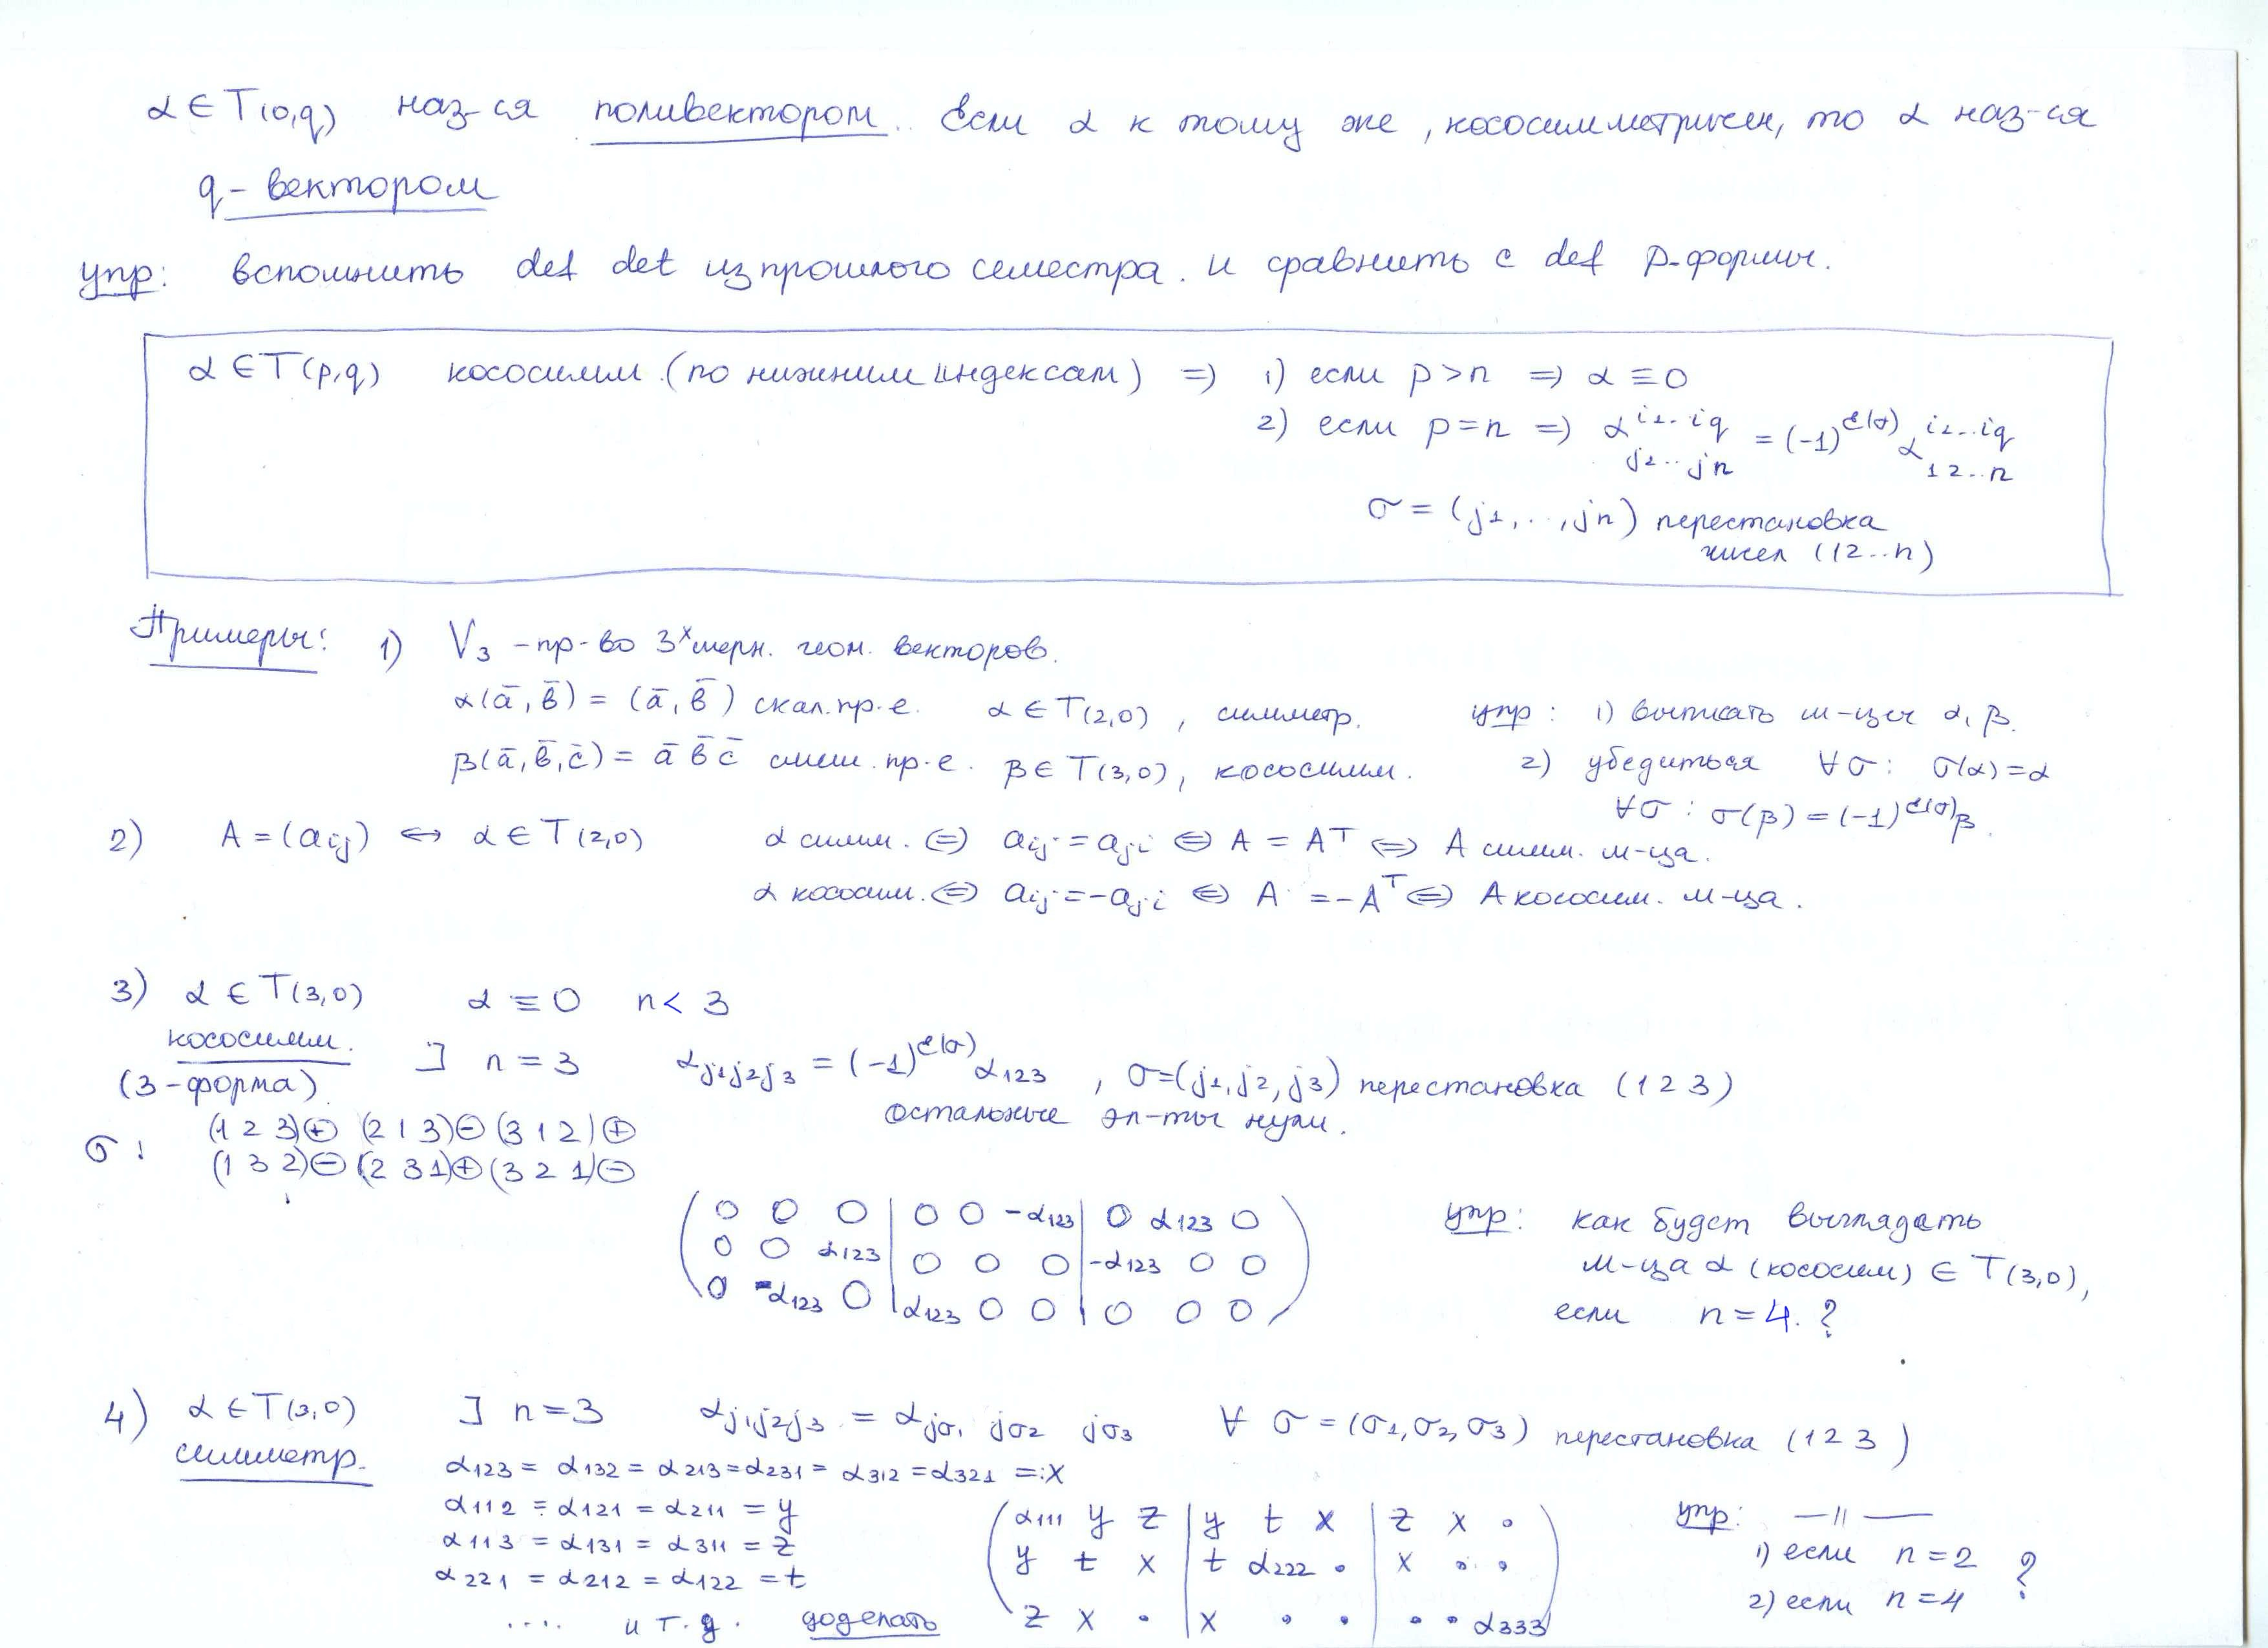
\includegraphics[height=0.49\textheight, width=\textwidth]{04006}	
		\n			
		
		
	\subsection{Операции альтернирования и симметрирования тензоров}
	 	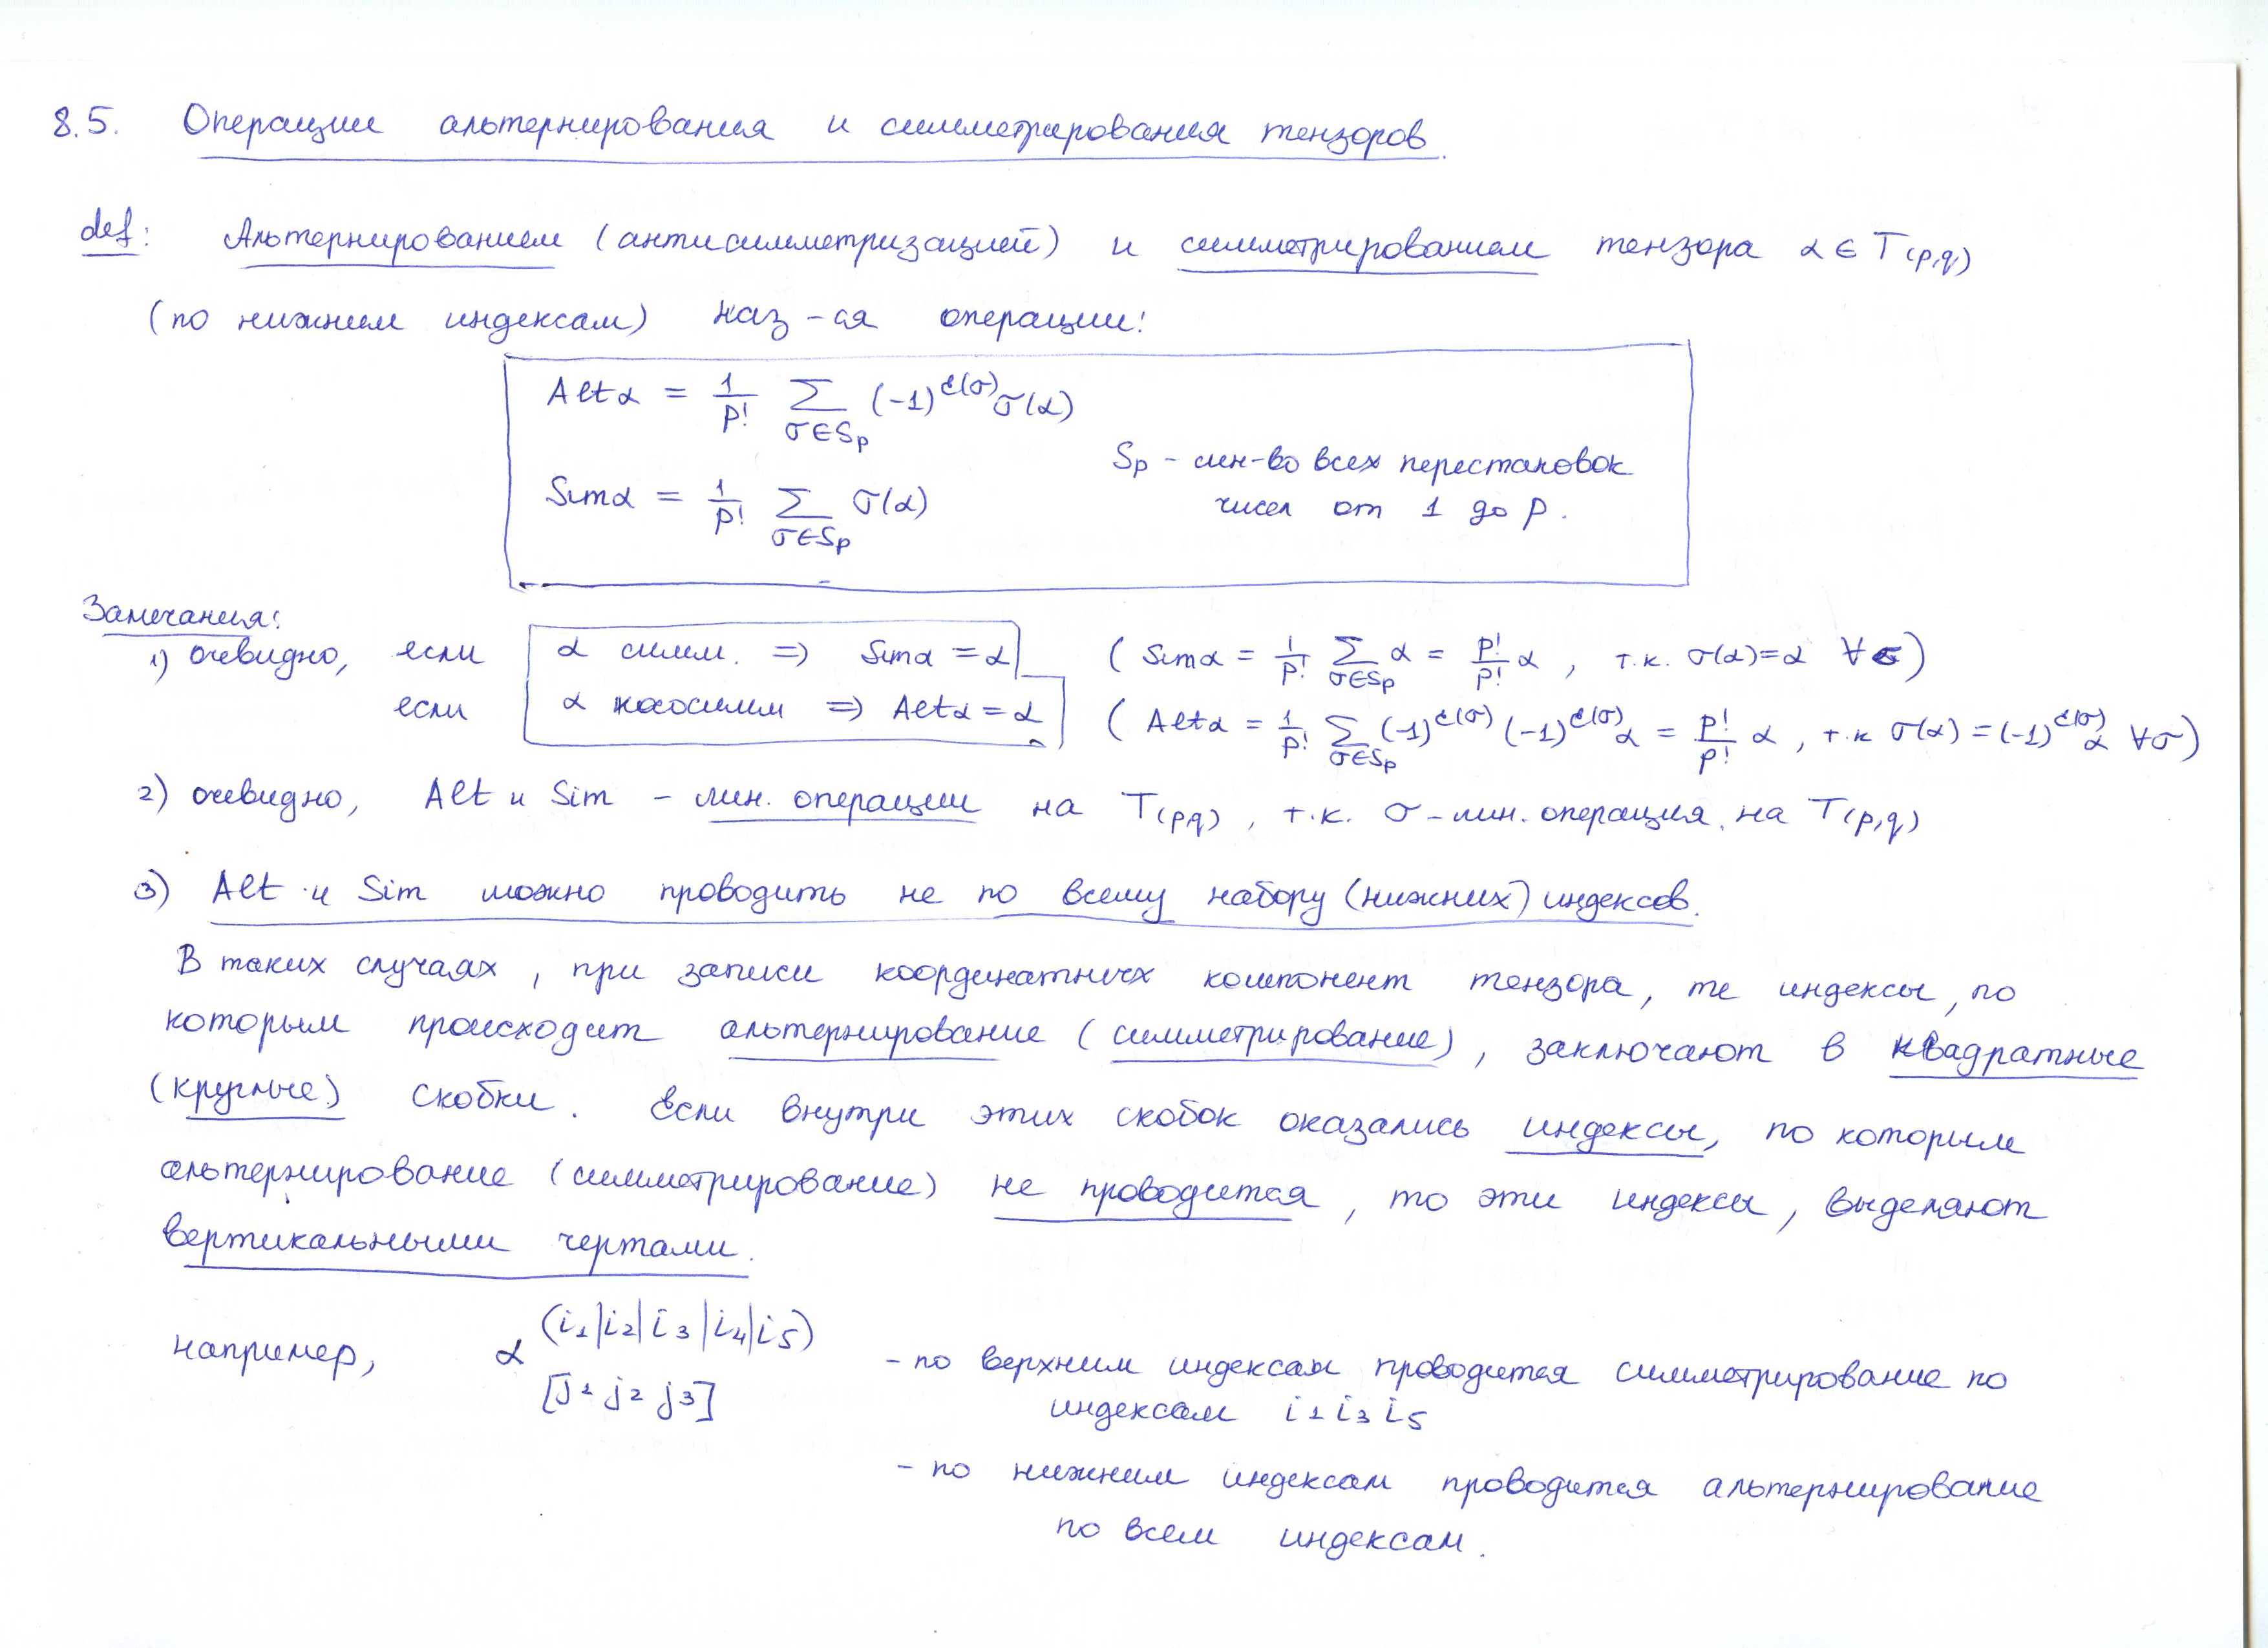
\includegraphics[height=0.49\textheight, width=\textwidth]{04007}	
		\n
		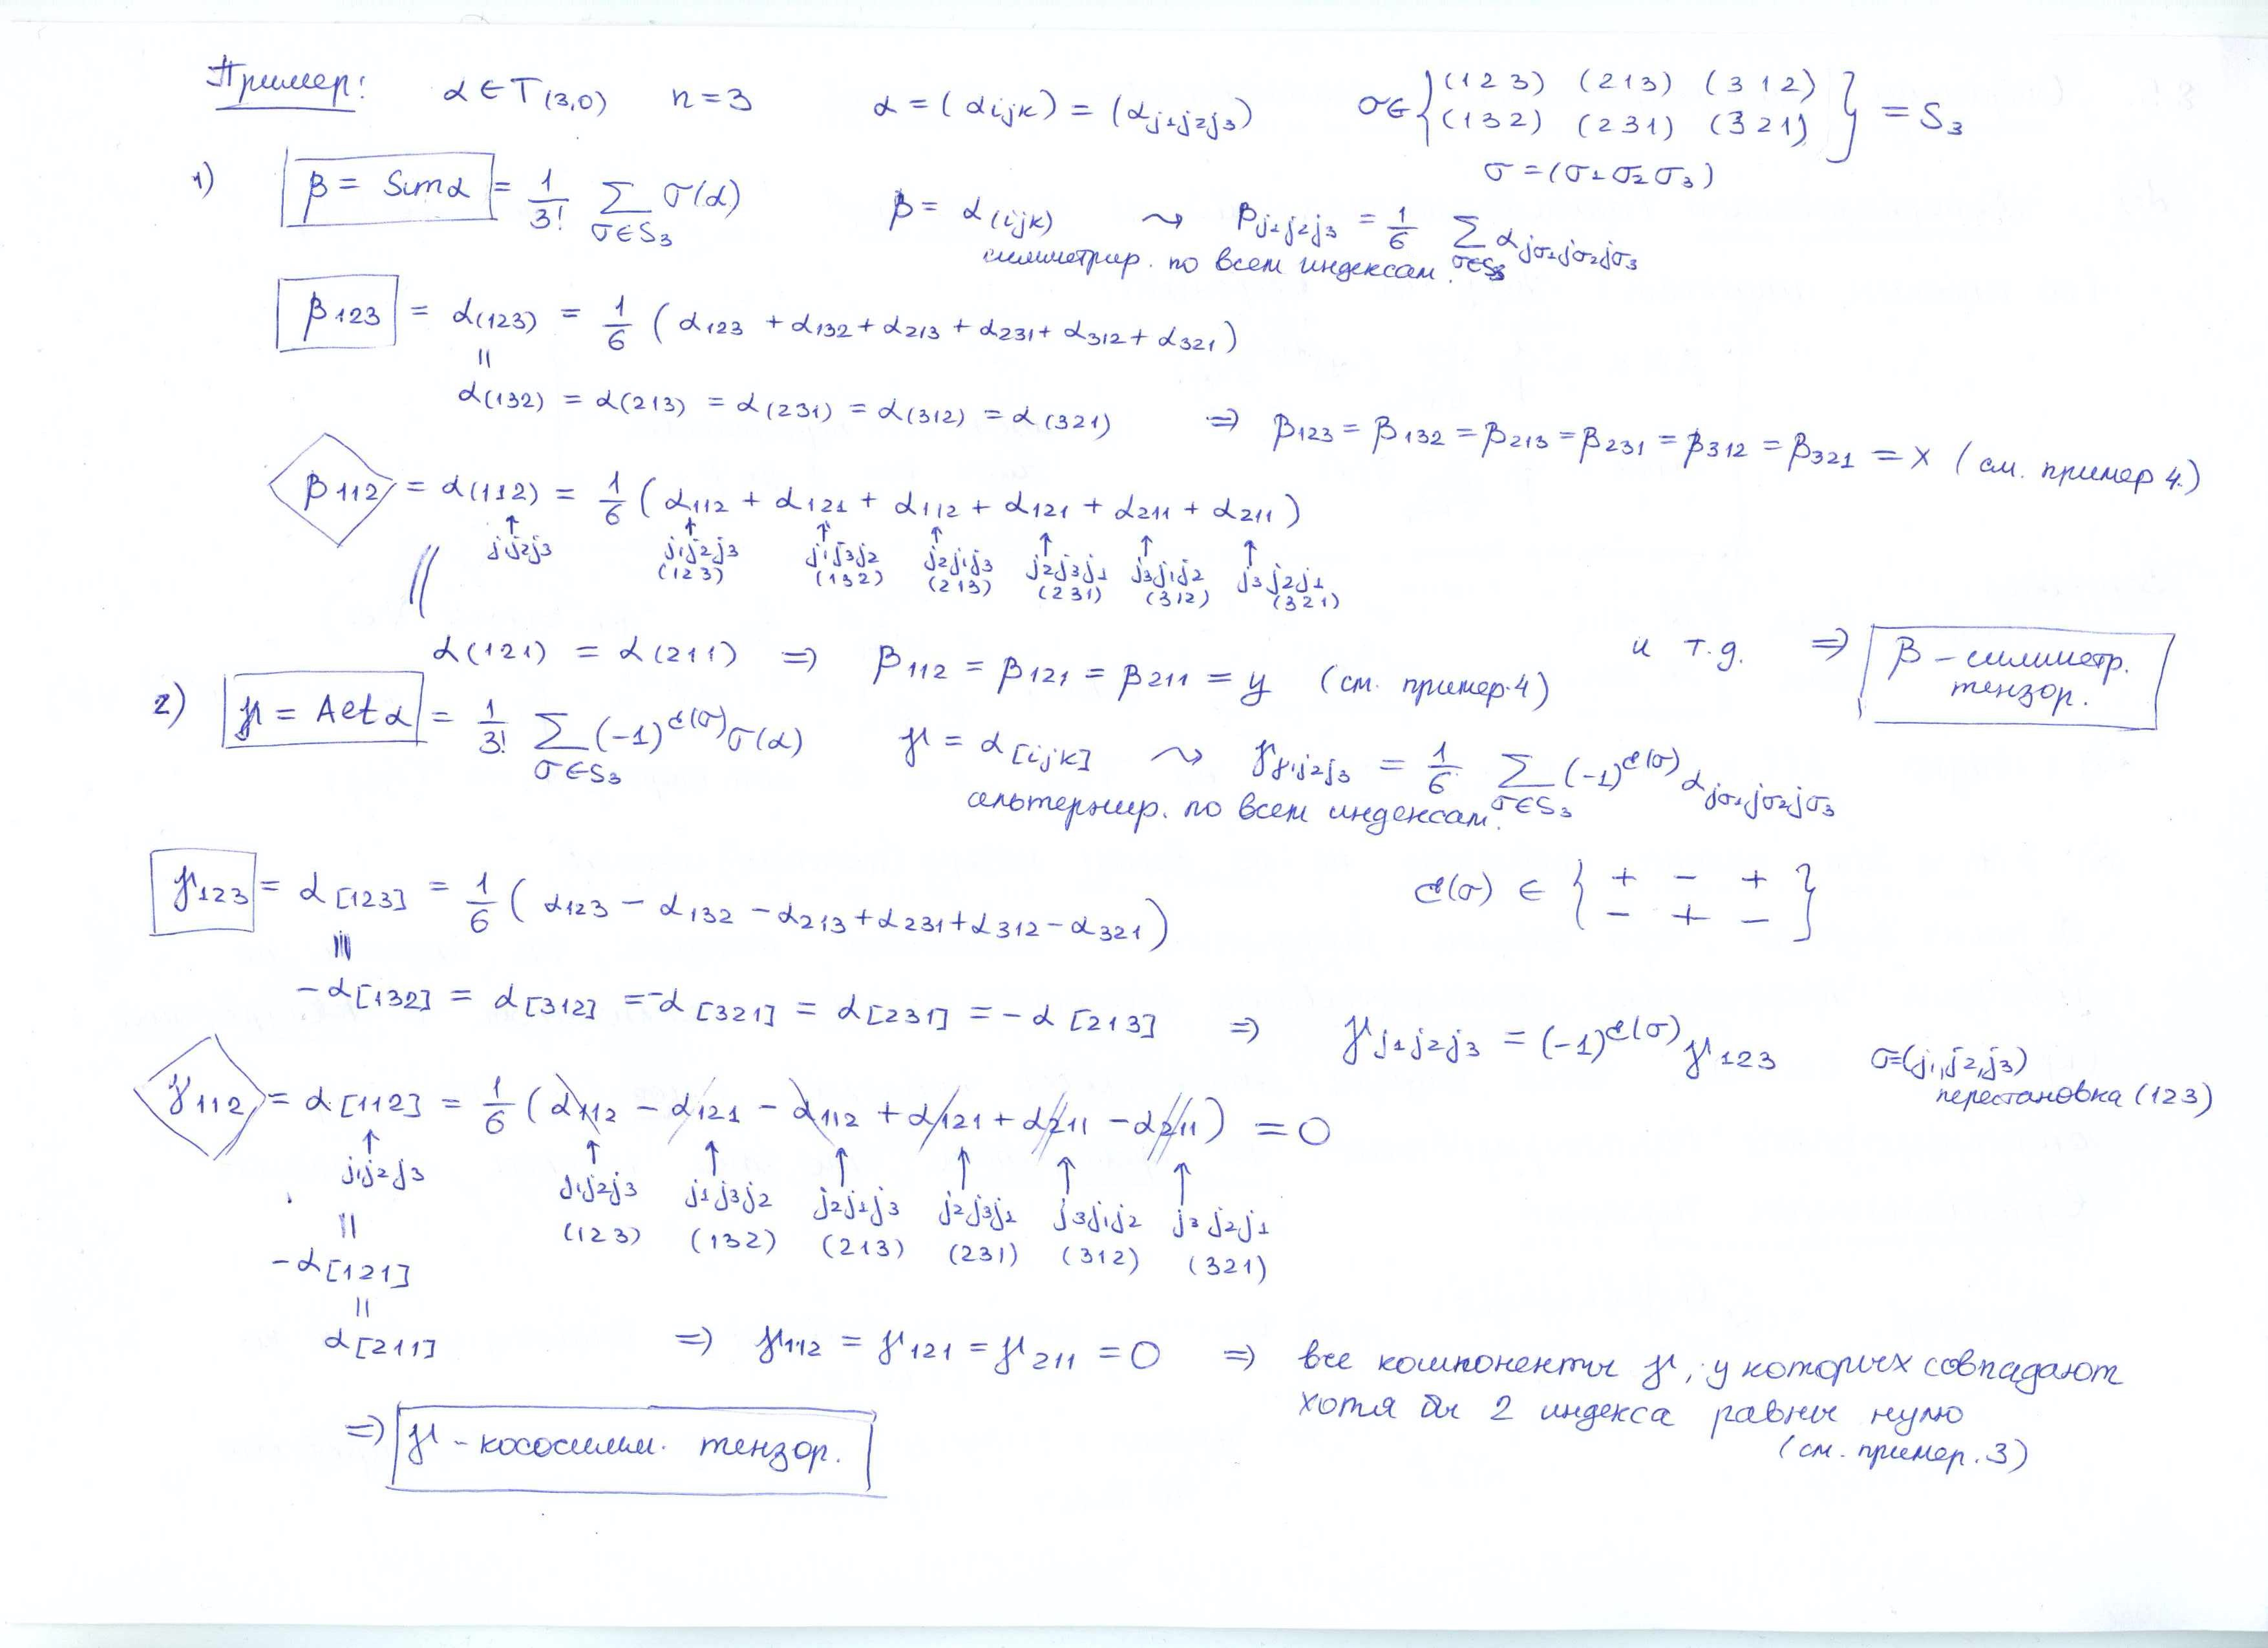
\includegraphics[height=0.49\textheight, width=\textwidth]{04008}	
		\n
		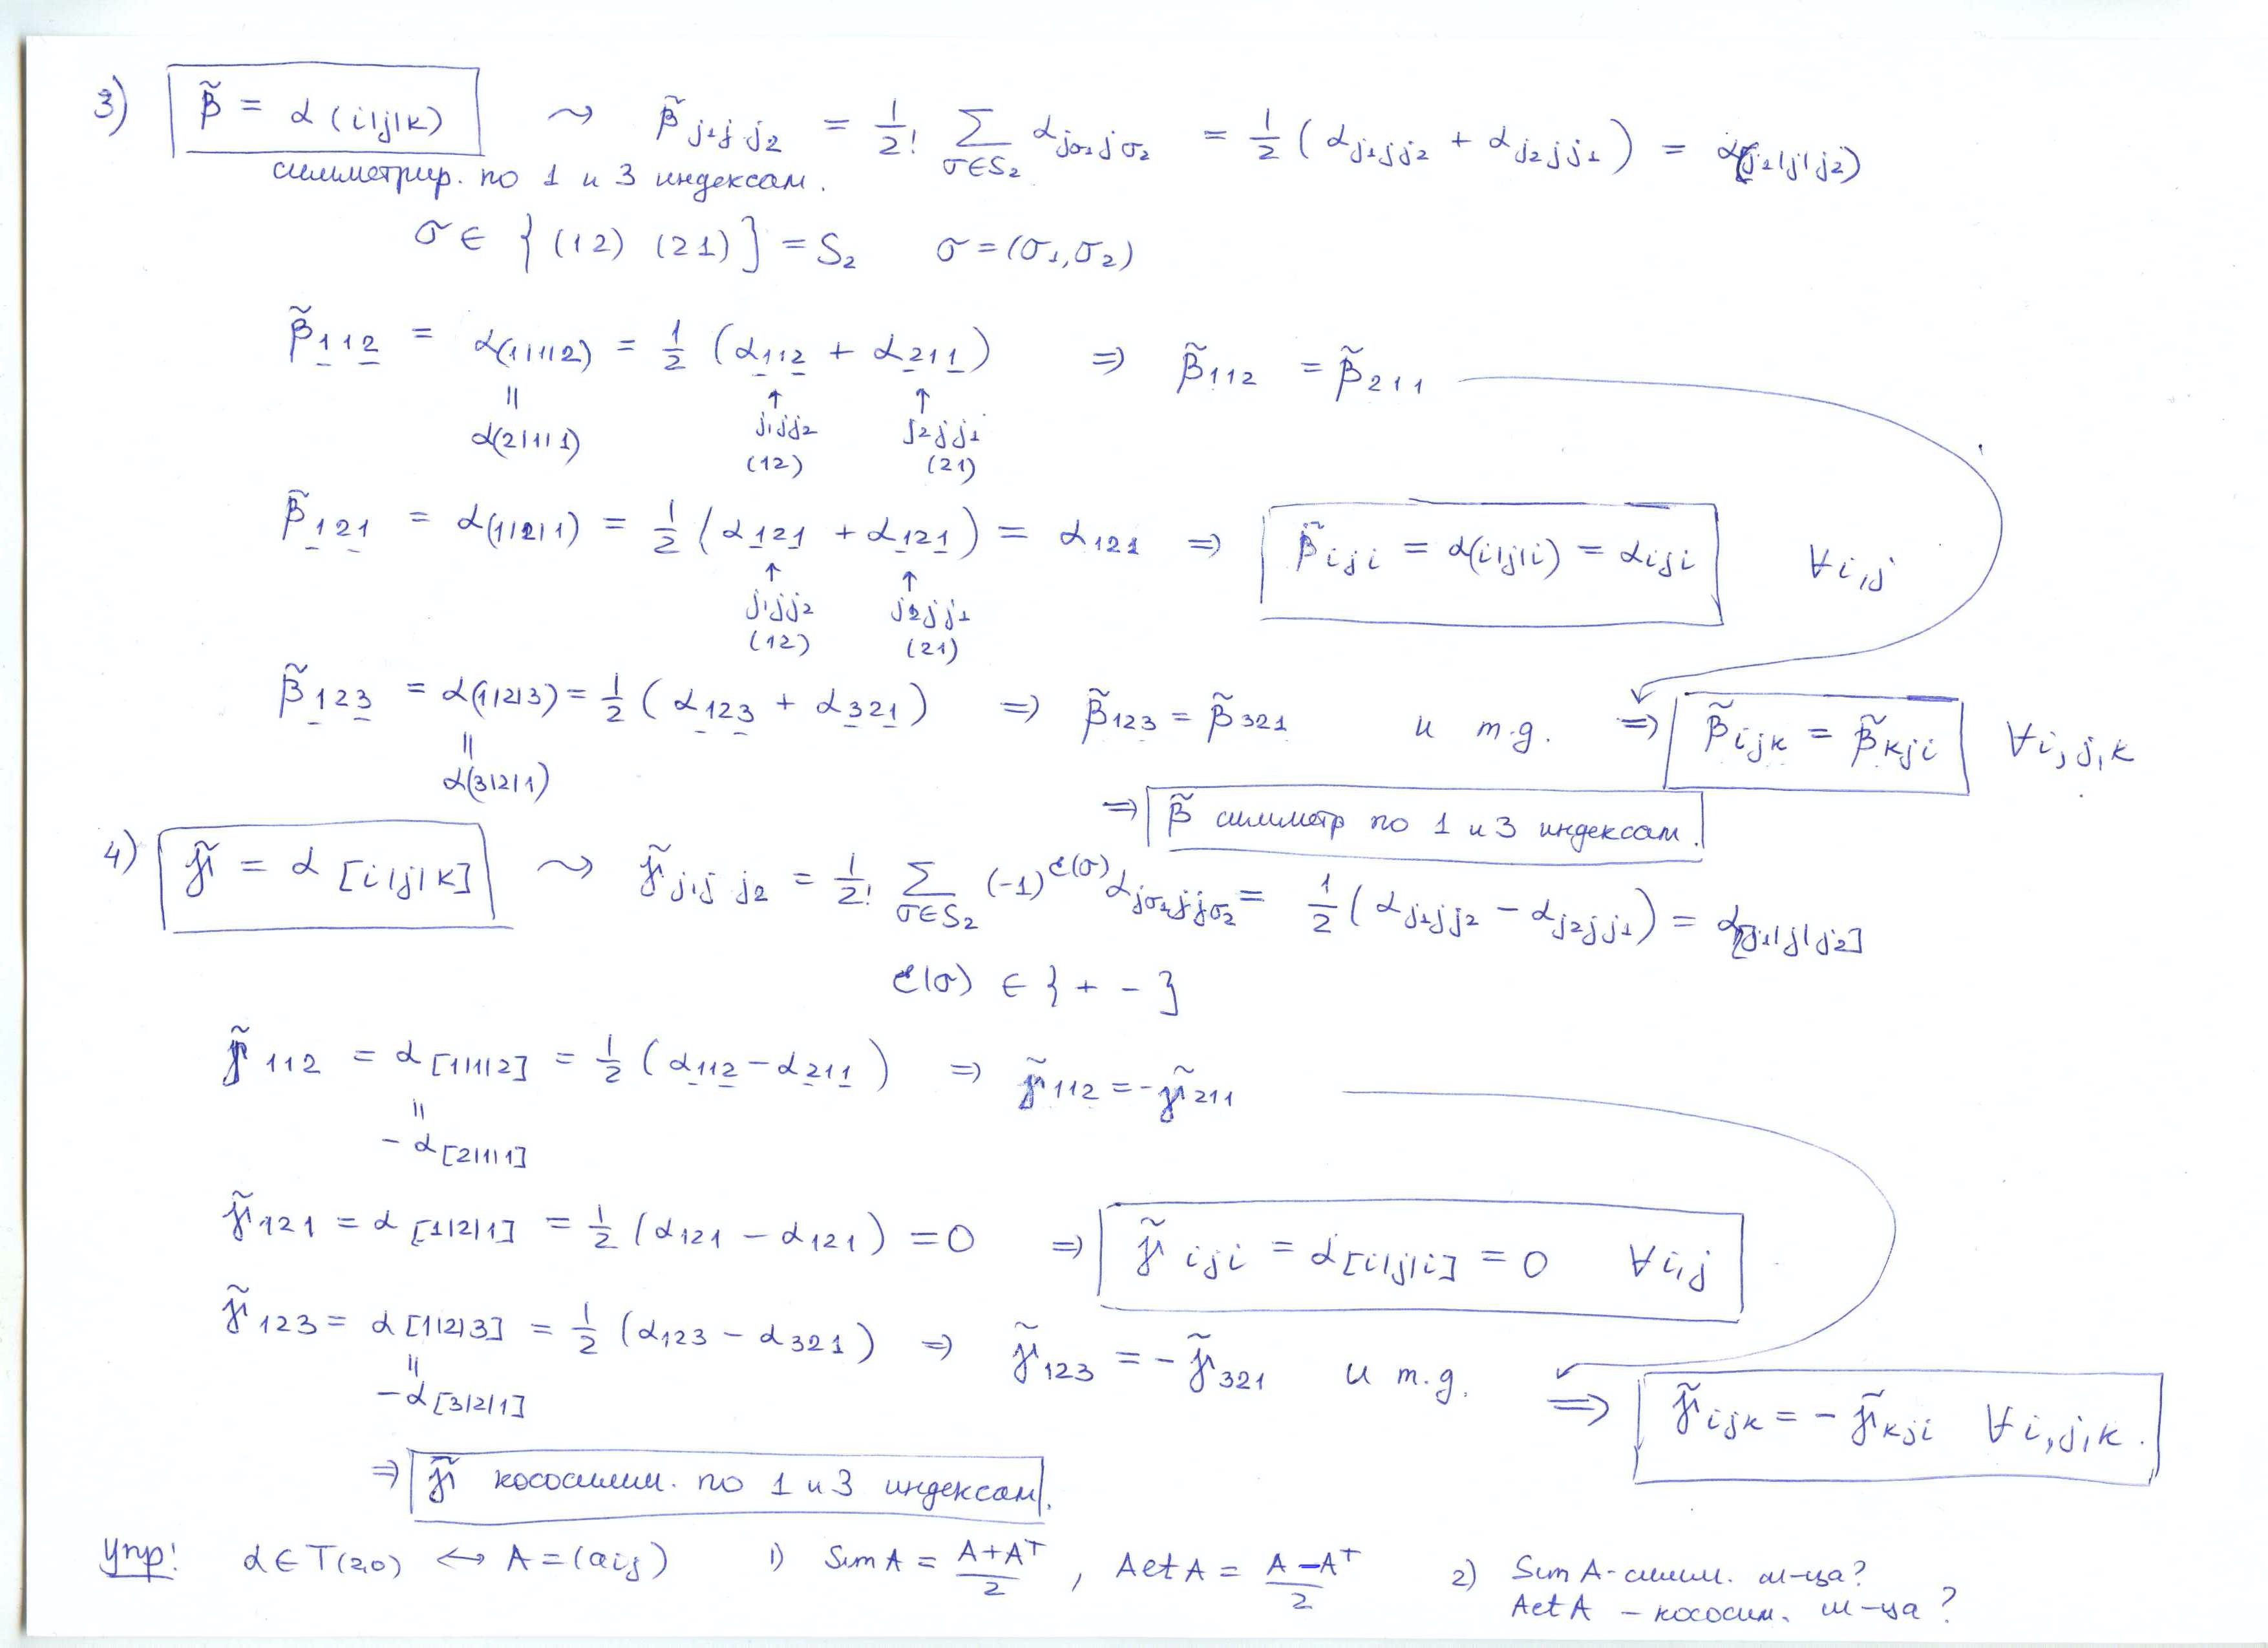
\includegraphics[height=0.49\textheight, width=\textwidth]{04009}
		\n
		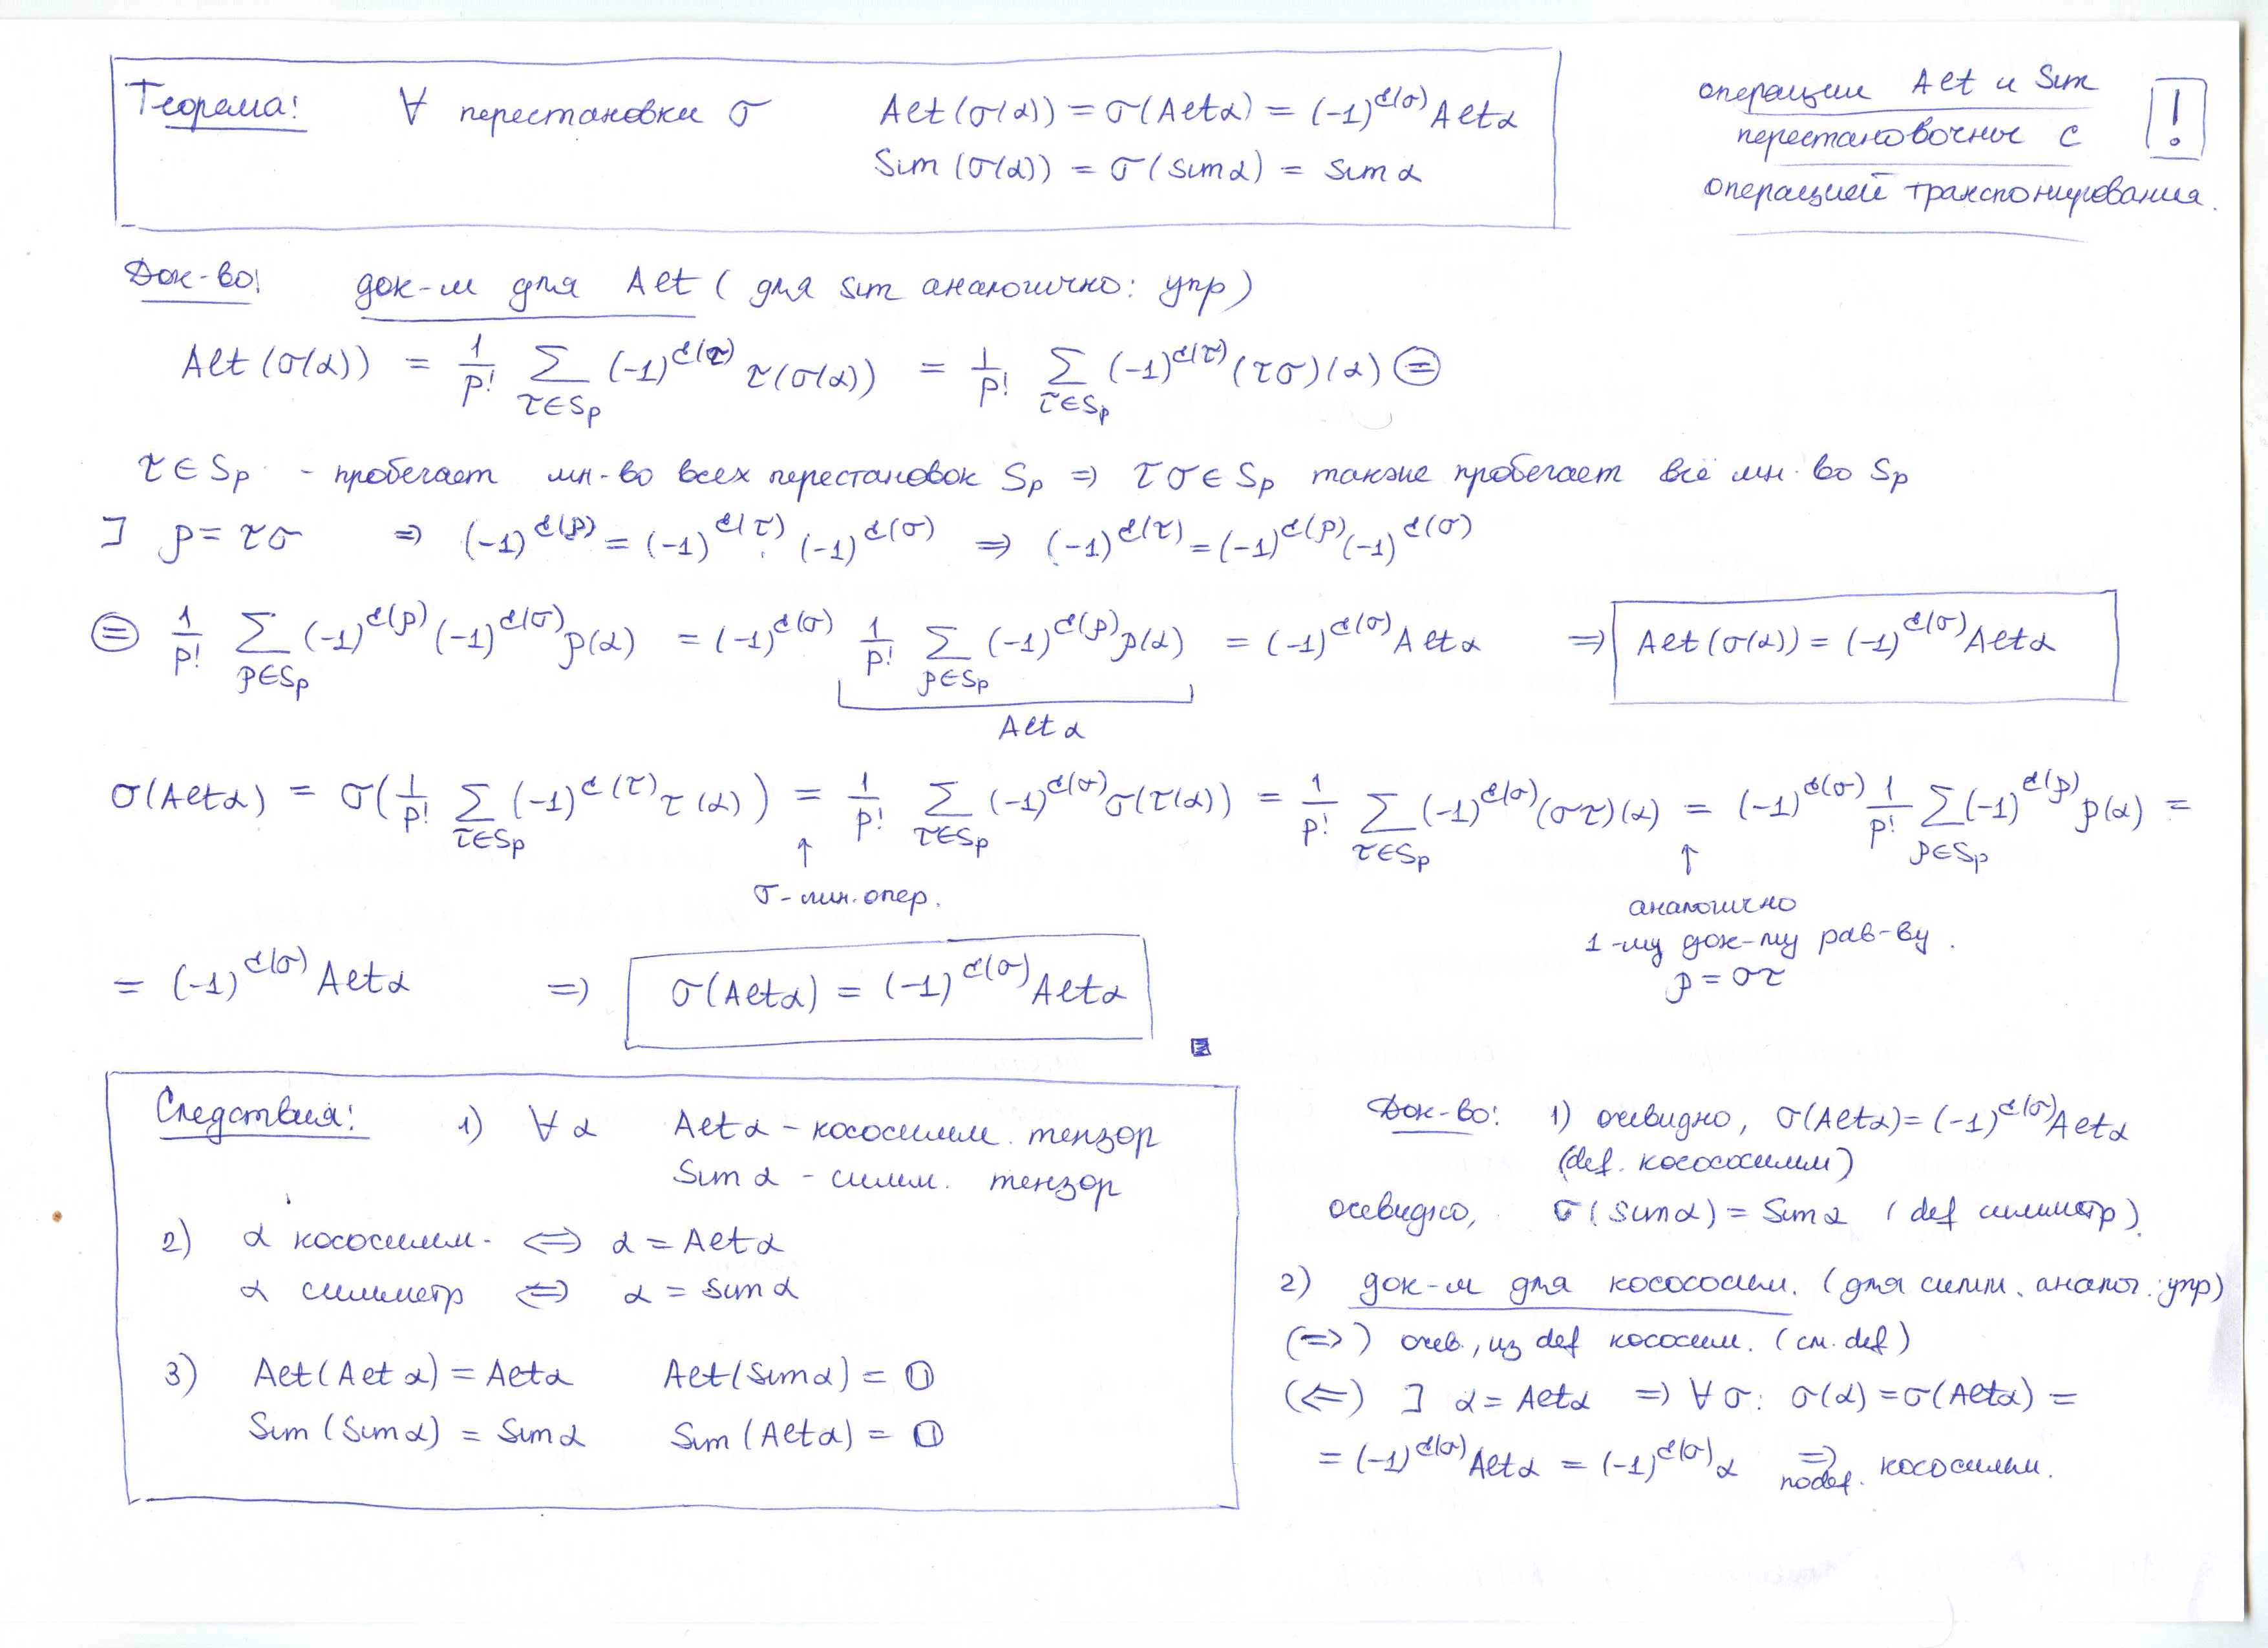
\includegraphics[height=0.49\textheight, width=\textwidth]{05001}
		\n
		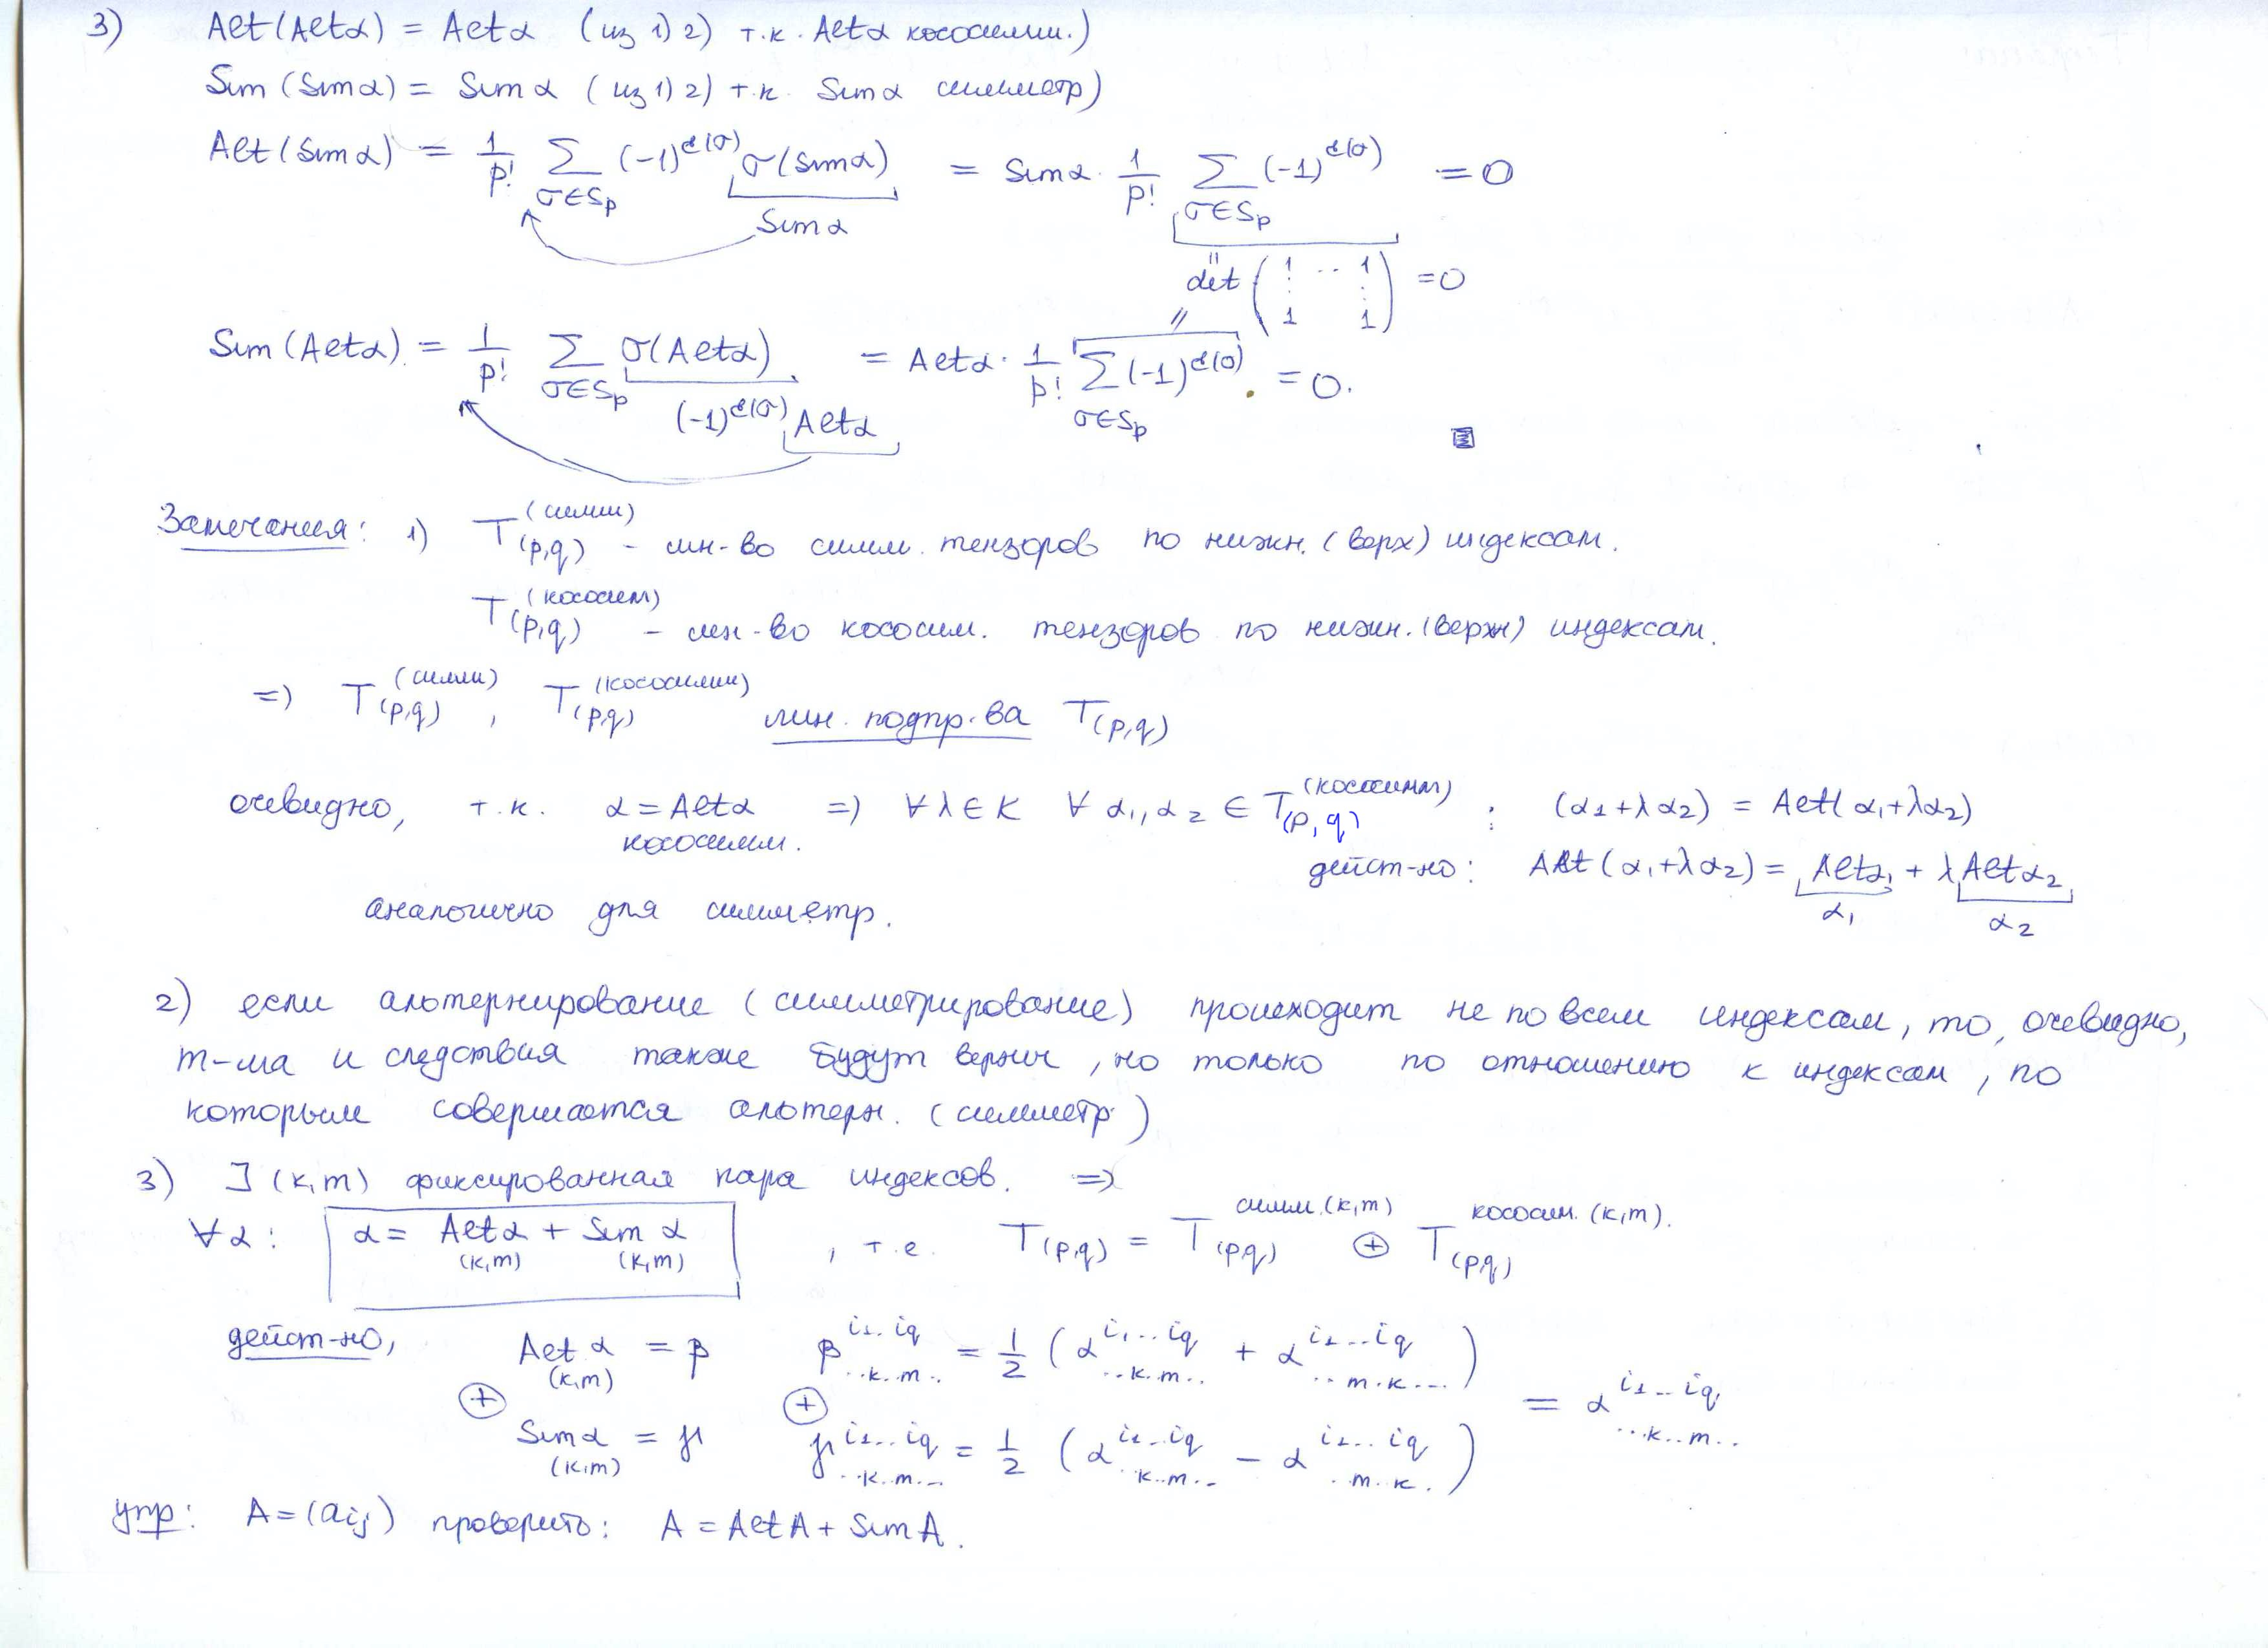
\includegraphics[height=0.49\textheight, width=\textwidth]{05002}
	\subsection{$p$-формы. Внешнее произведение $p$-формы.}
		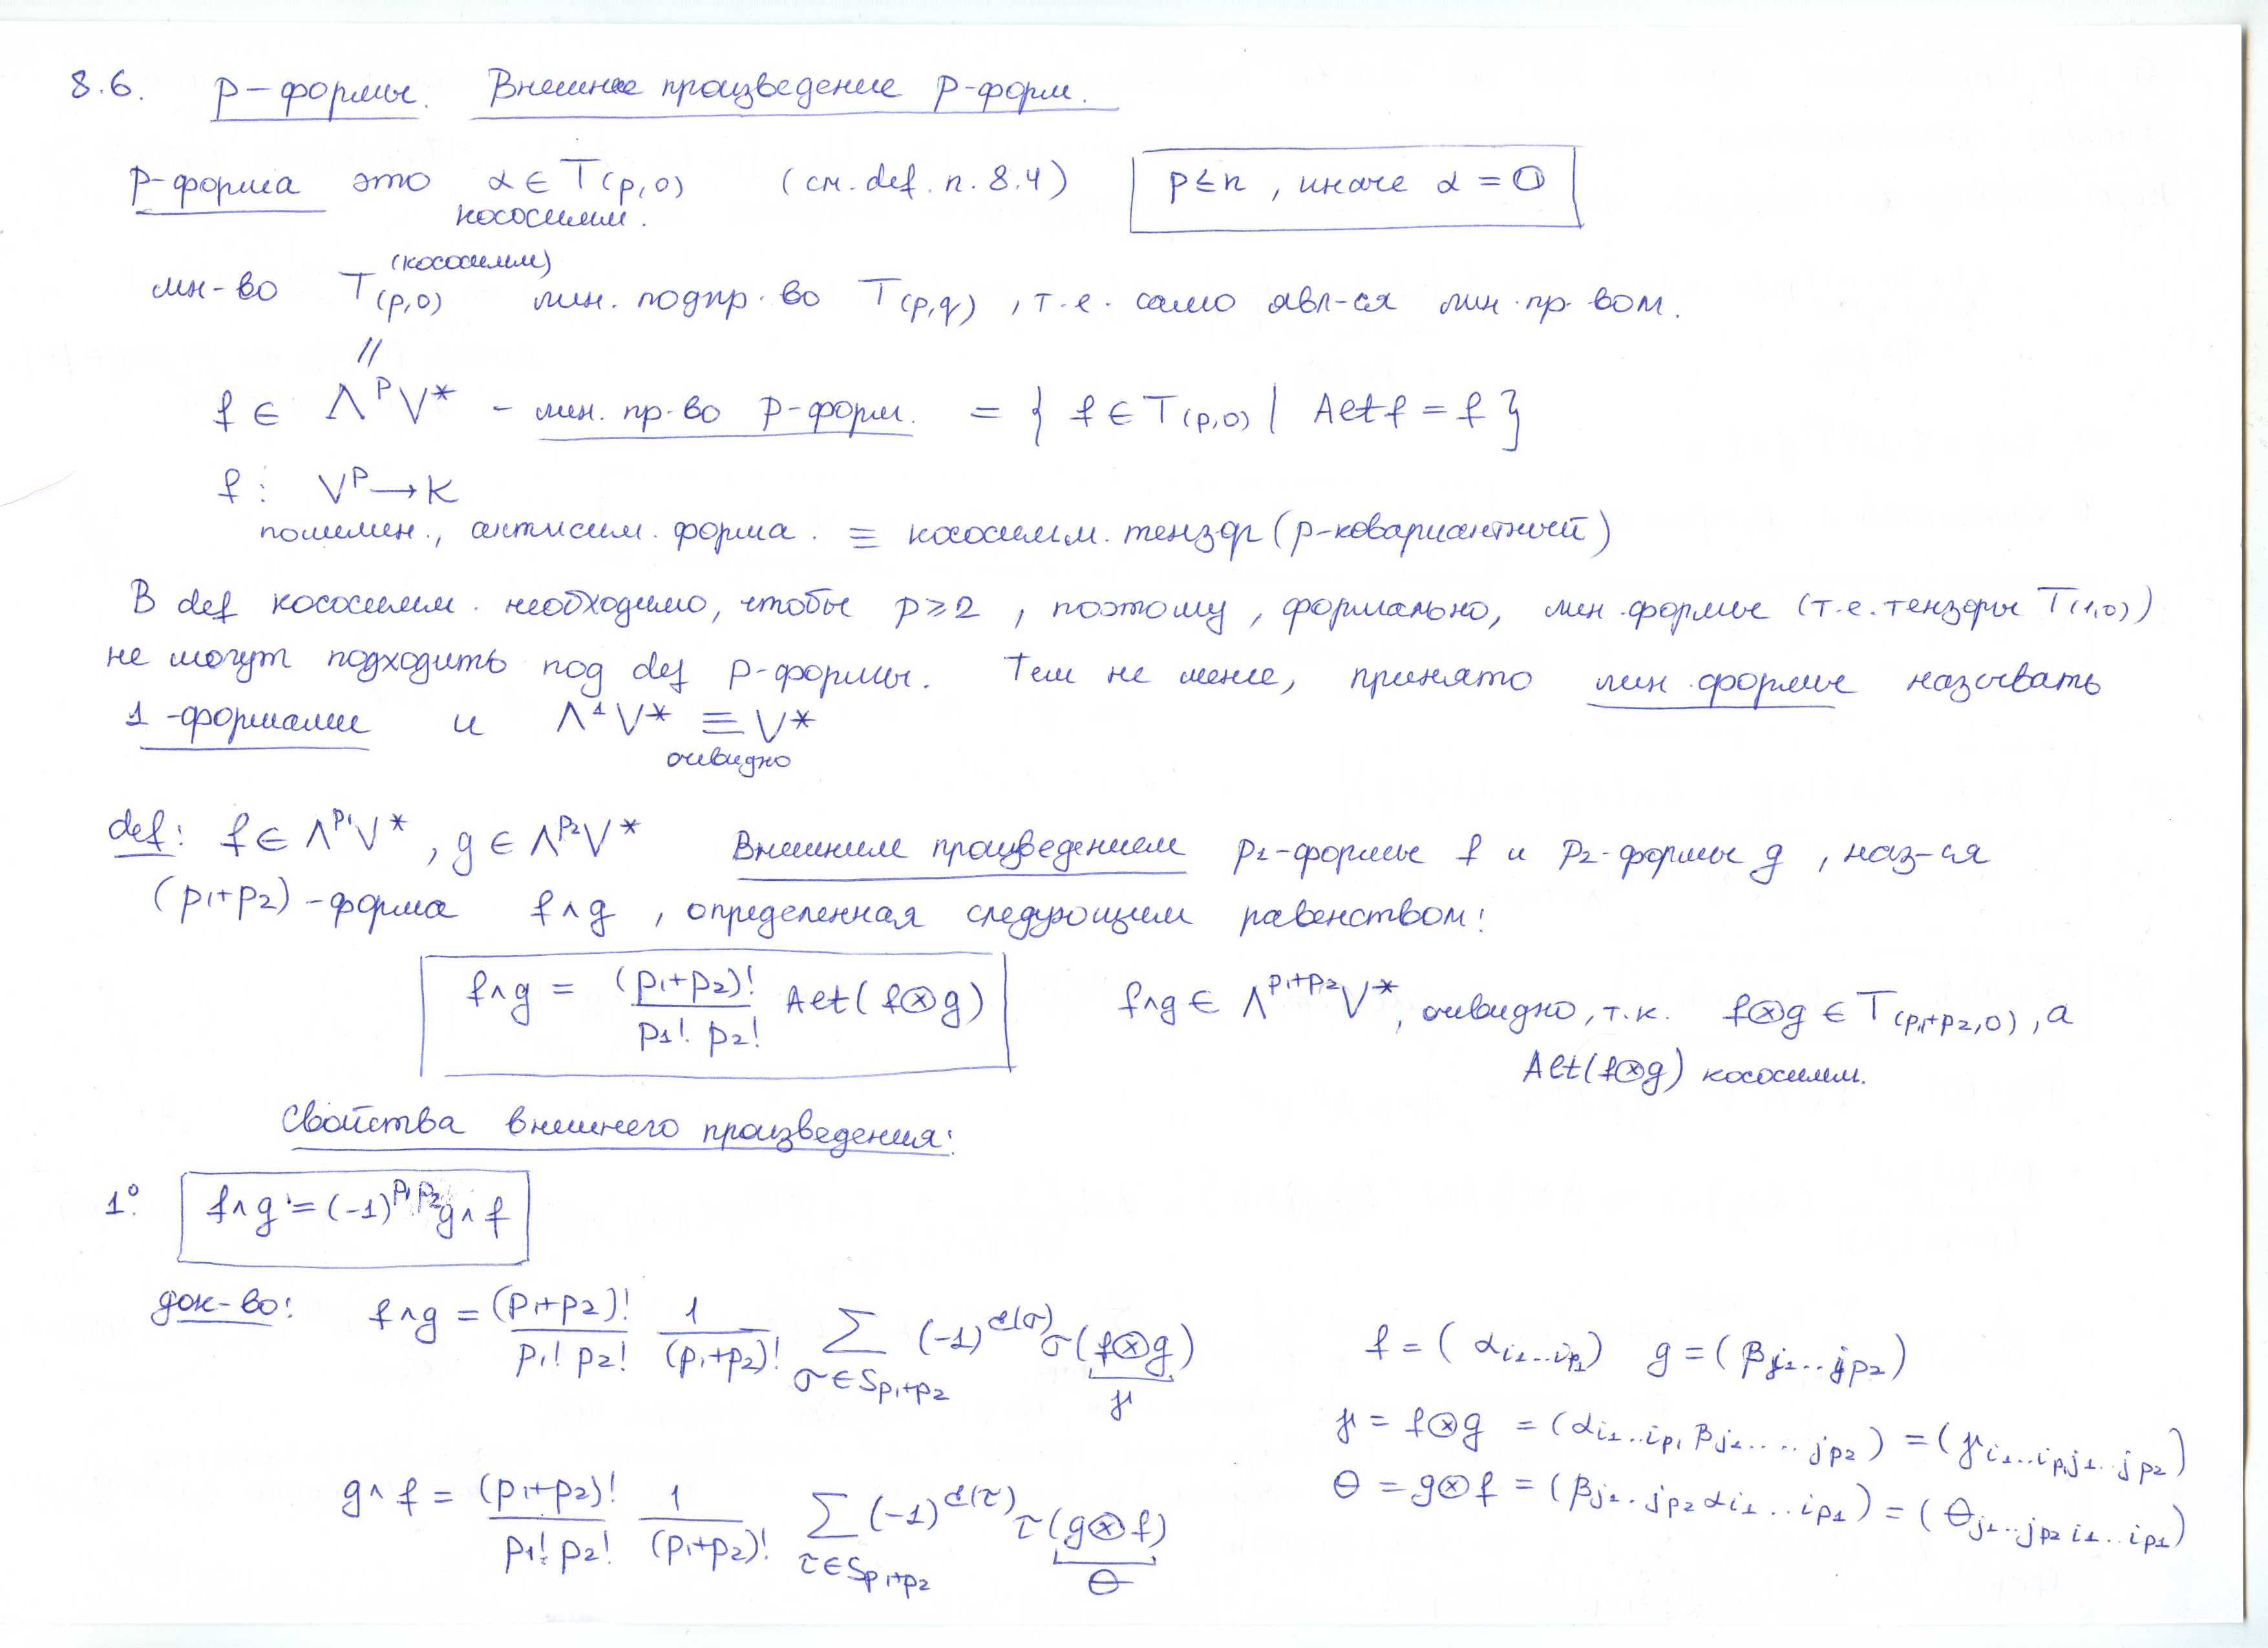
\includegraphics[height=0.49\textheight, width=\textwidth]{05003}
		\n
		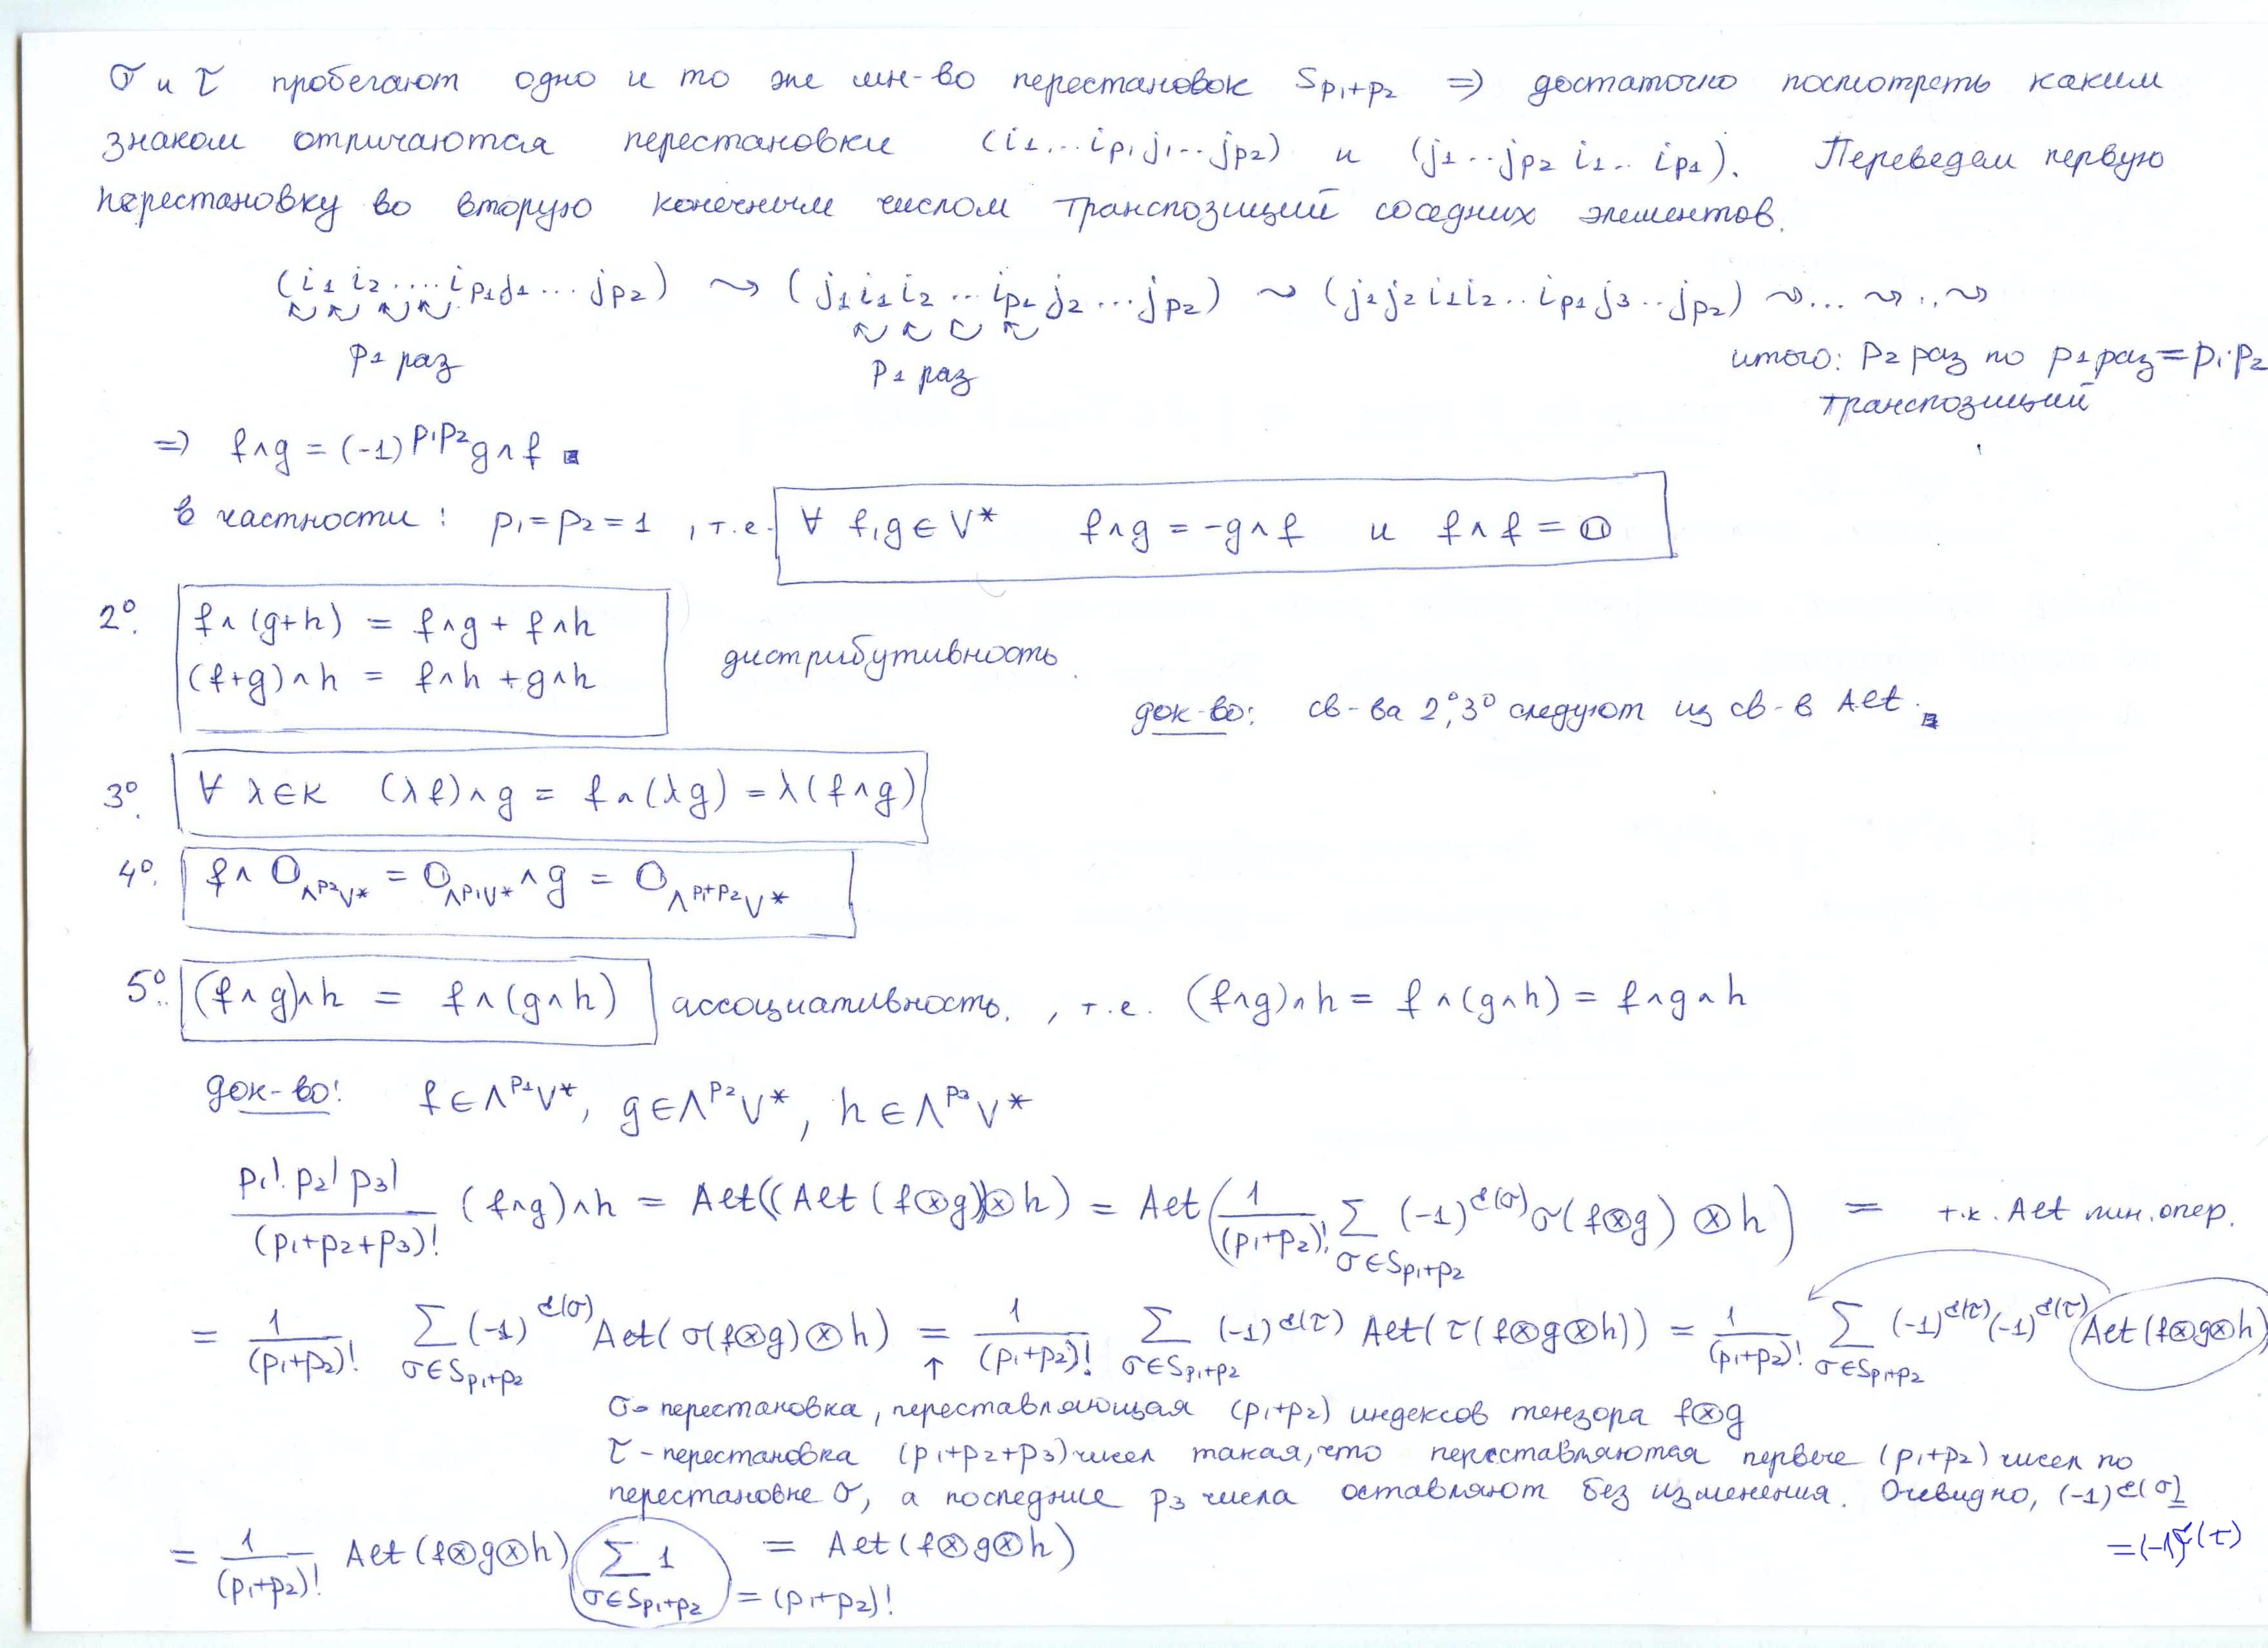
\includegraphics[height=0.49\textheight, width=\textwidth]{05004}
		\n
		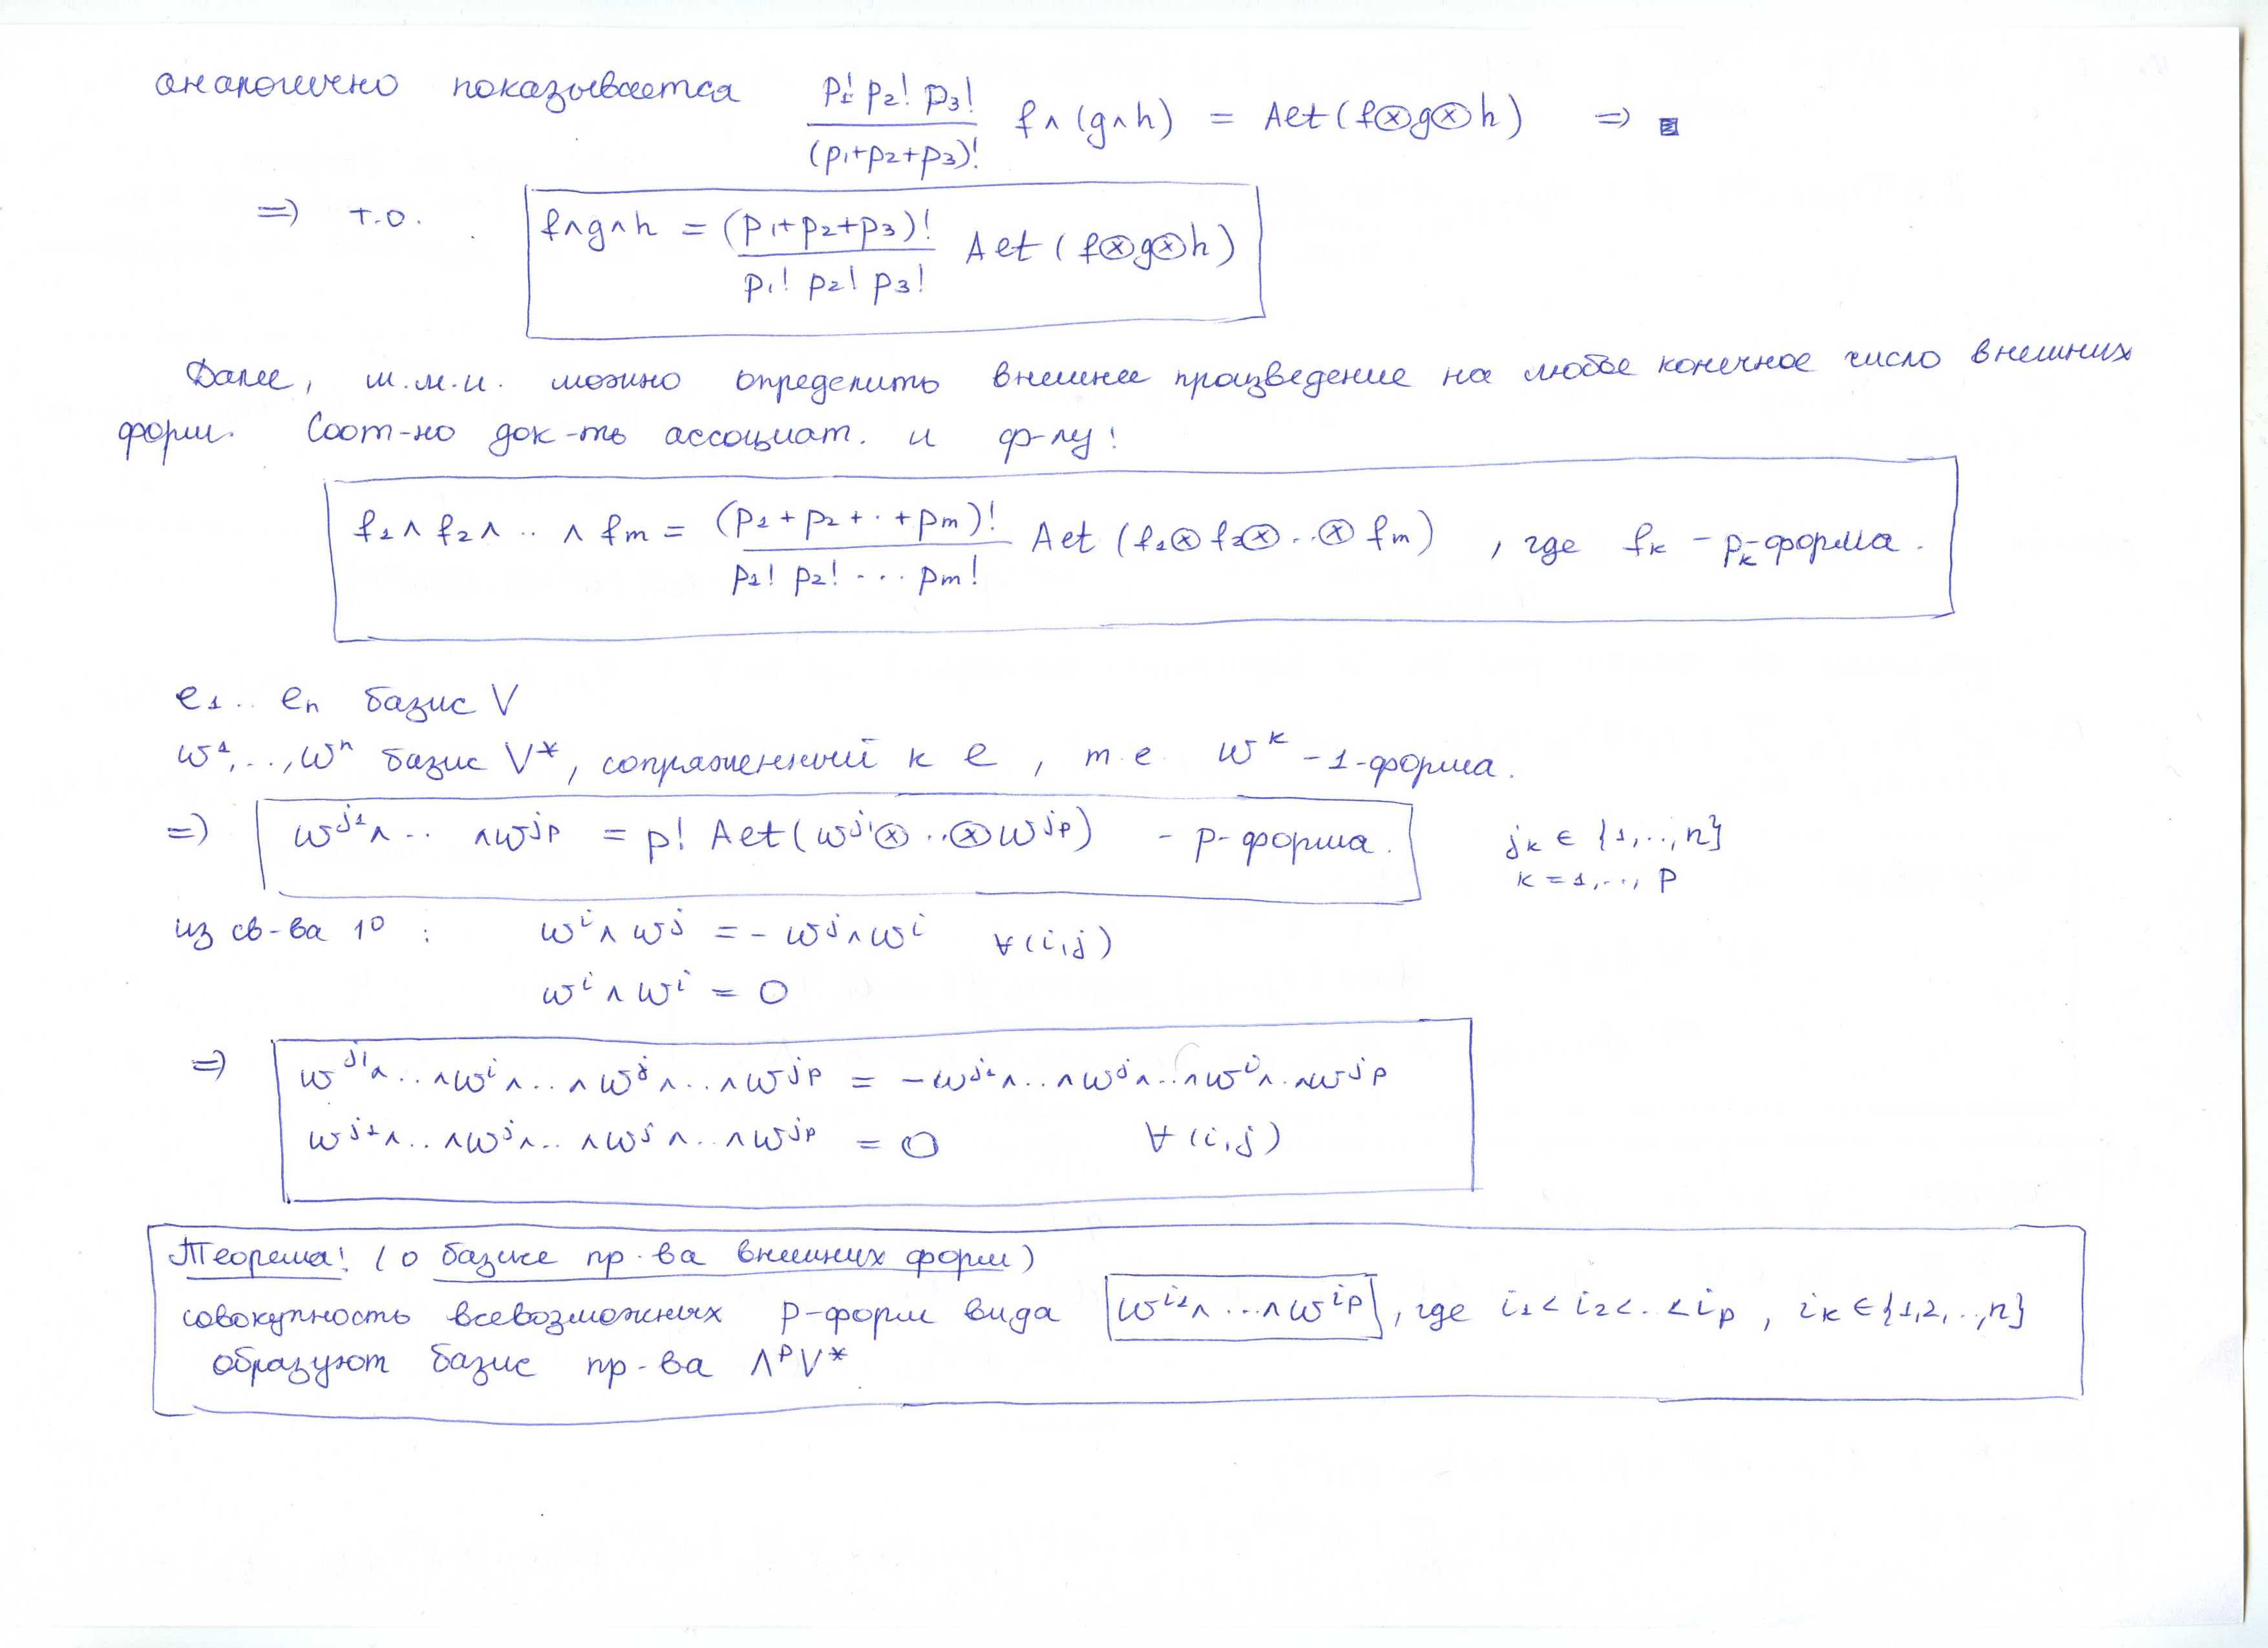
\includegraphics[height=0.49\textheight, width=\textwidth]{05005}
		\n
		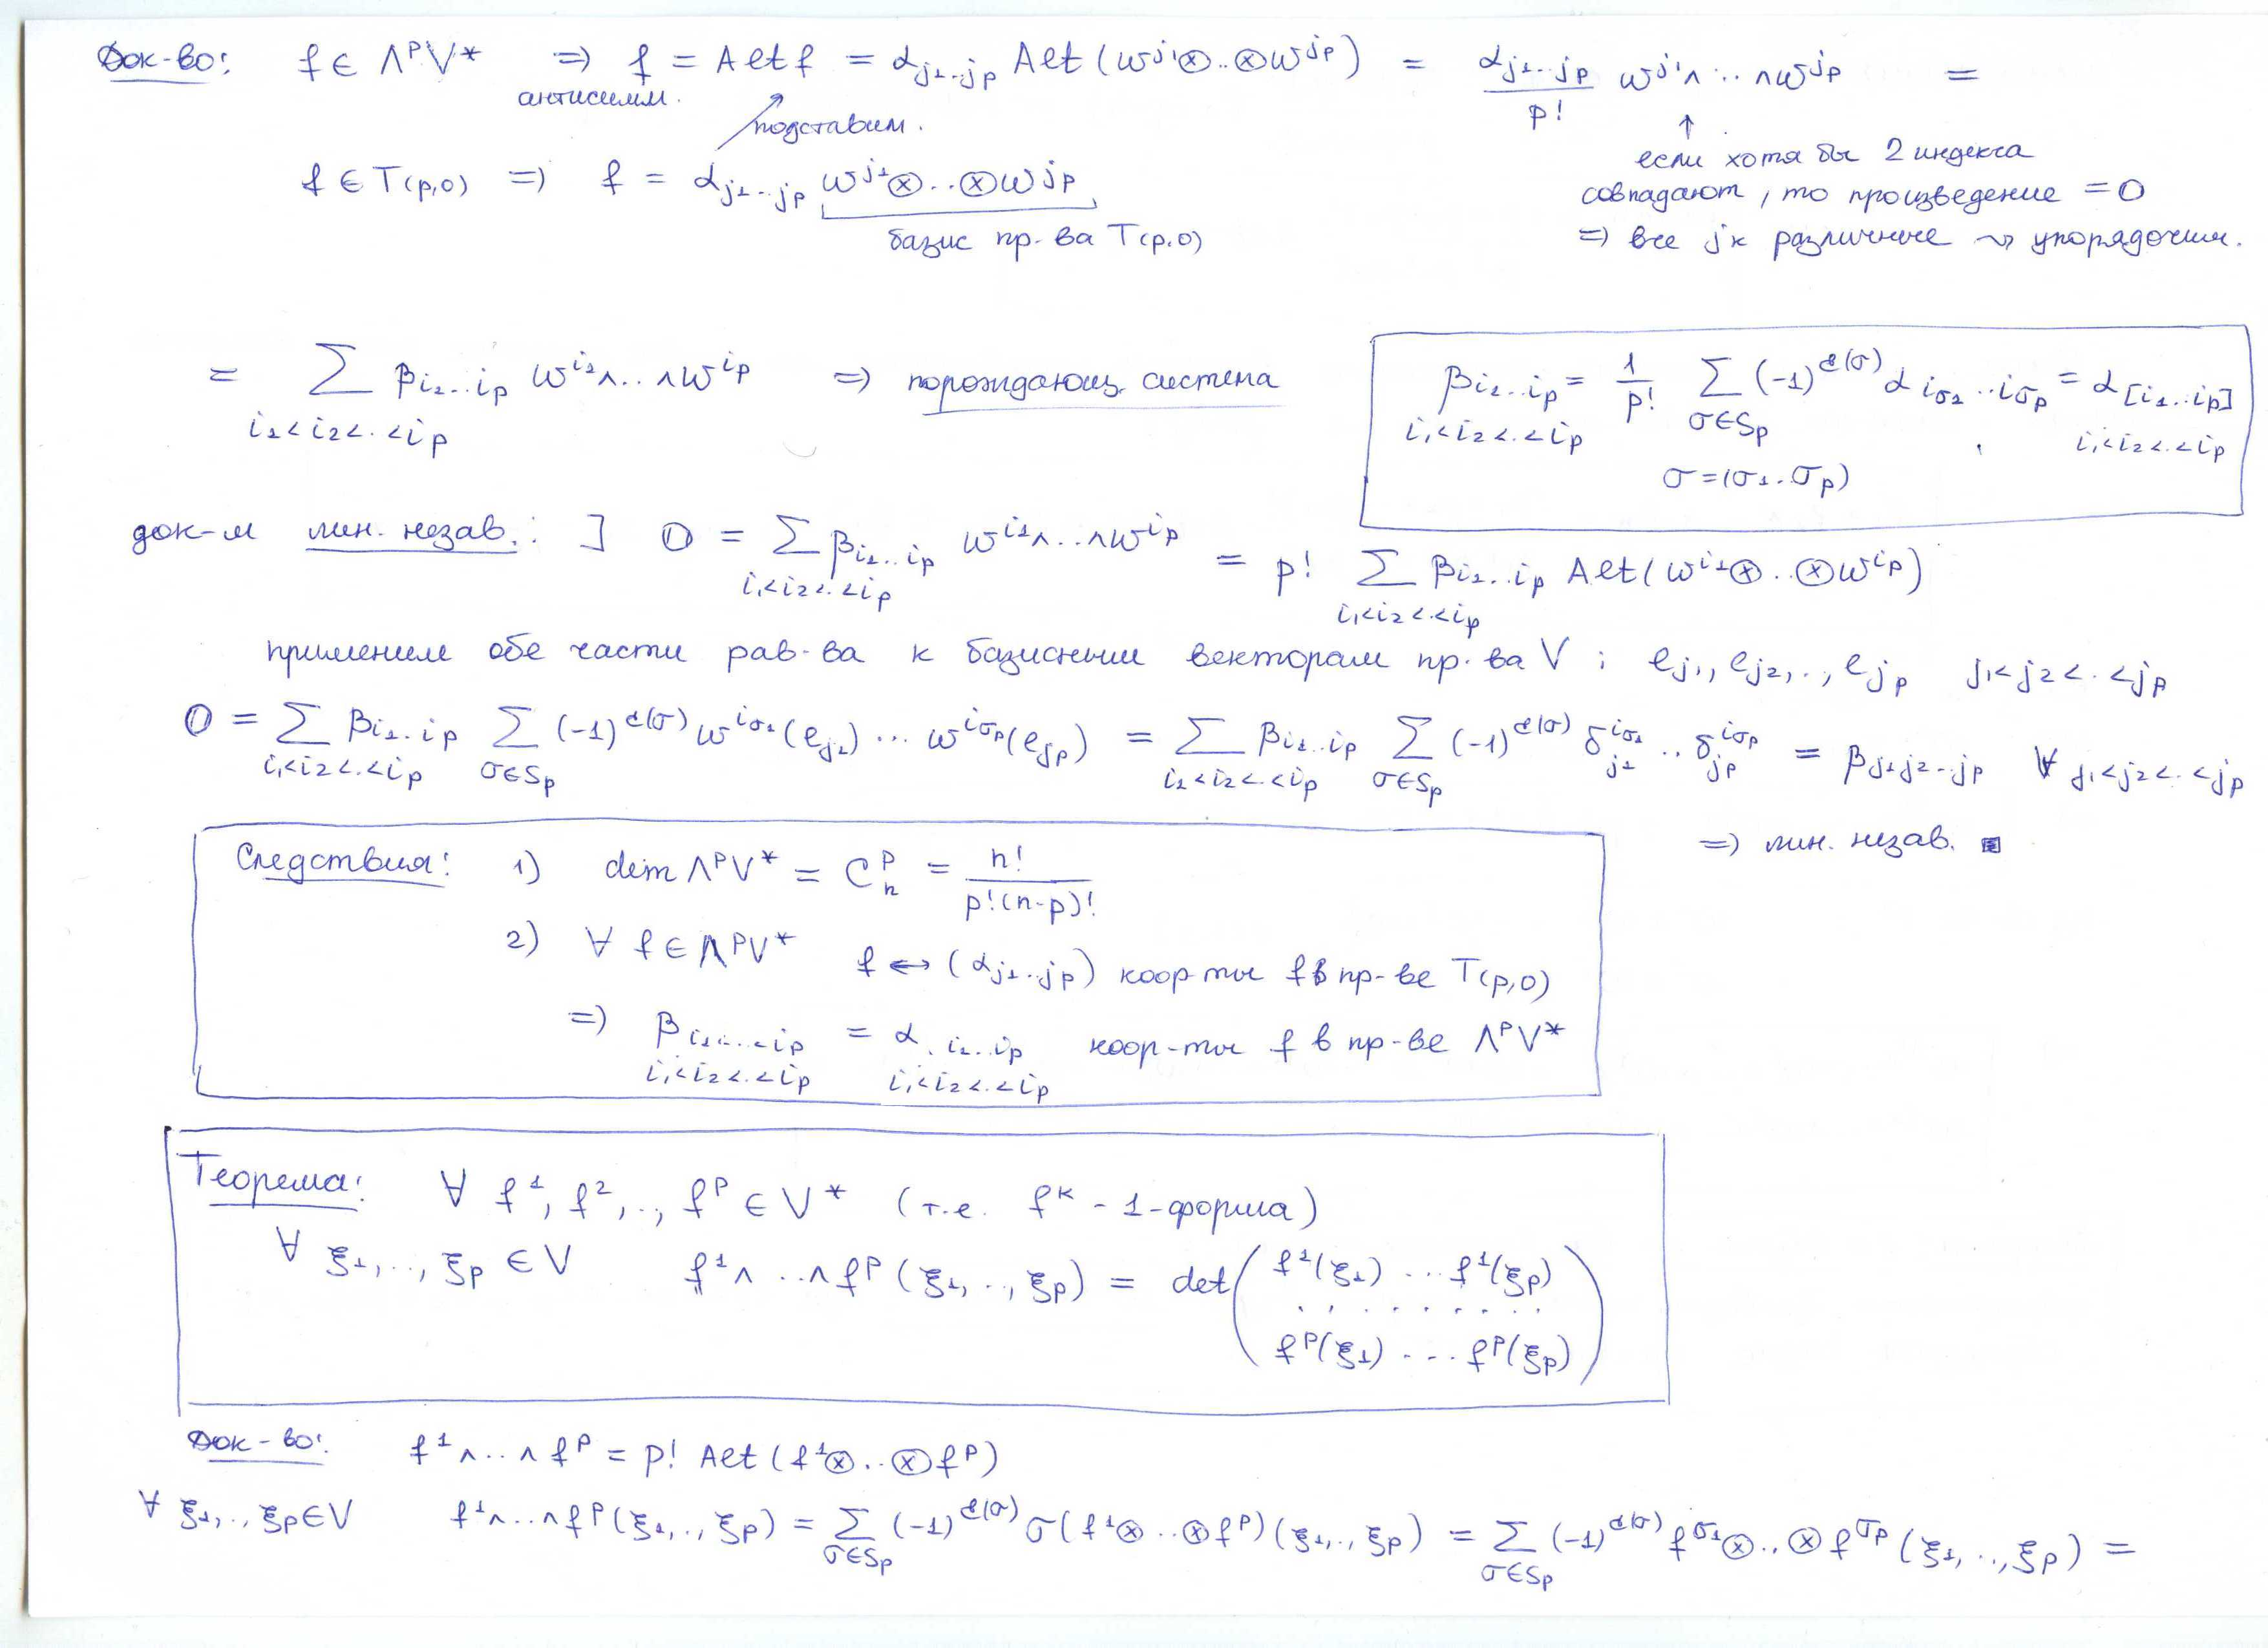
\includegraphics[height=0.49\textheight, width=\textwidth]{05006}
		\n
		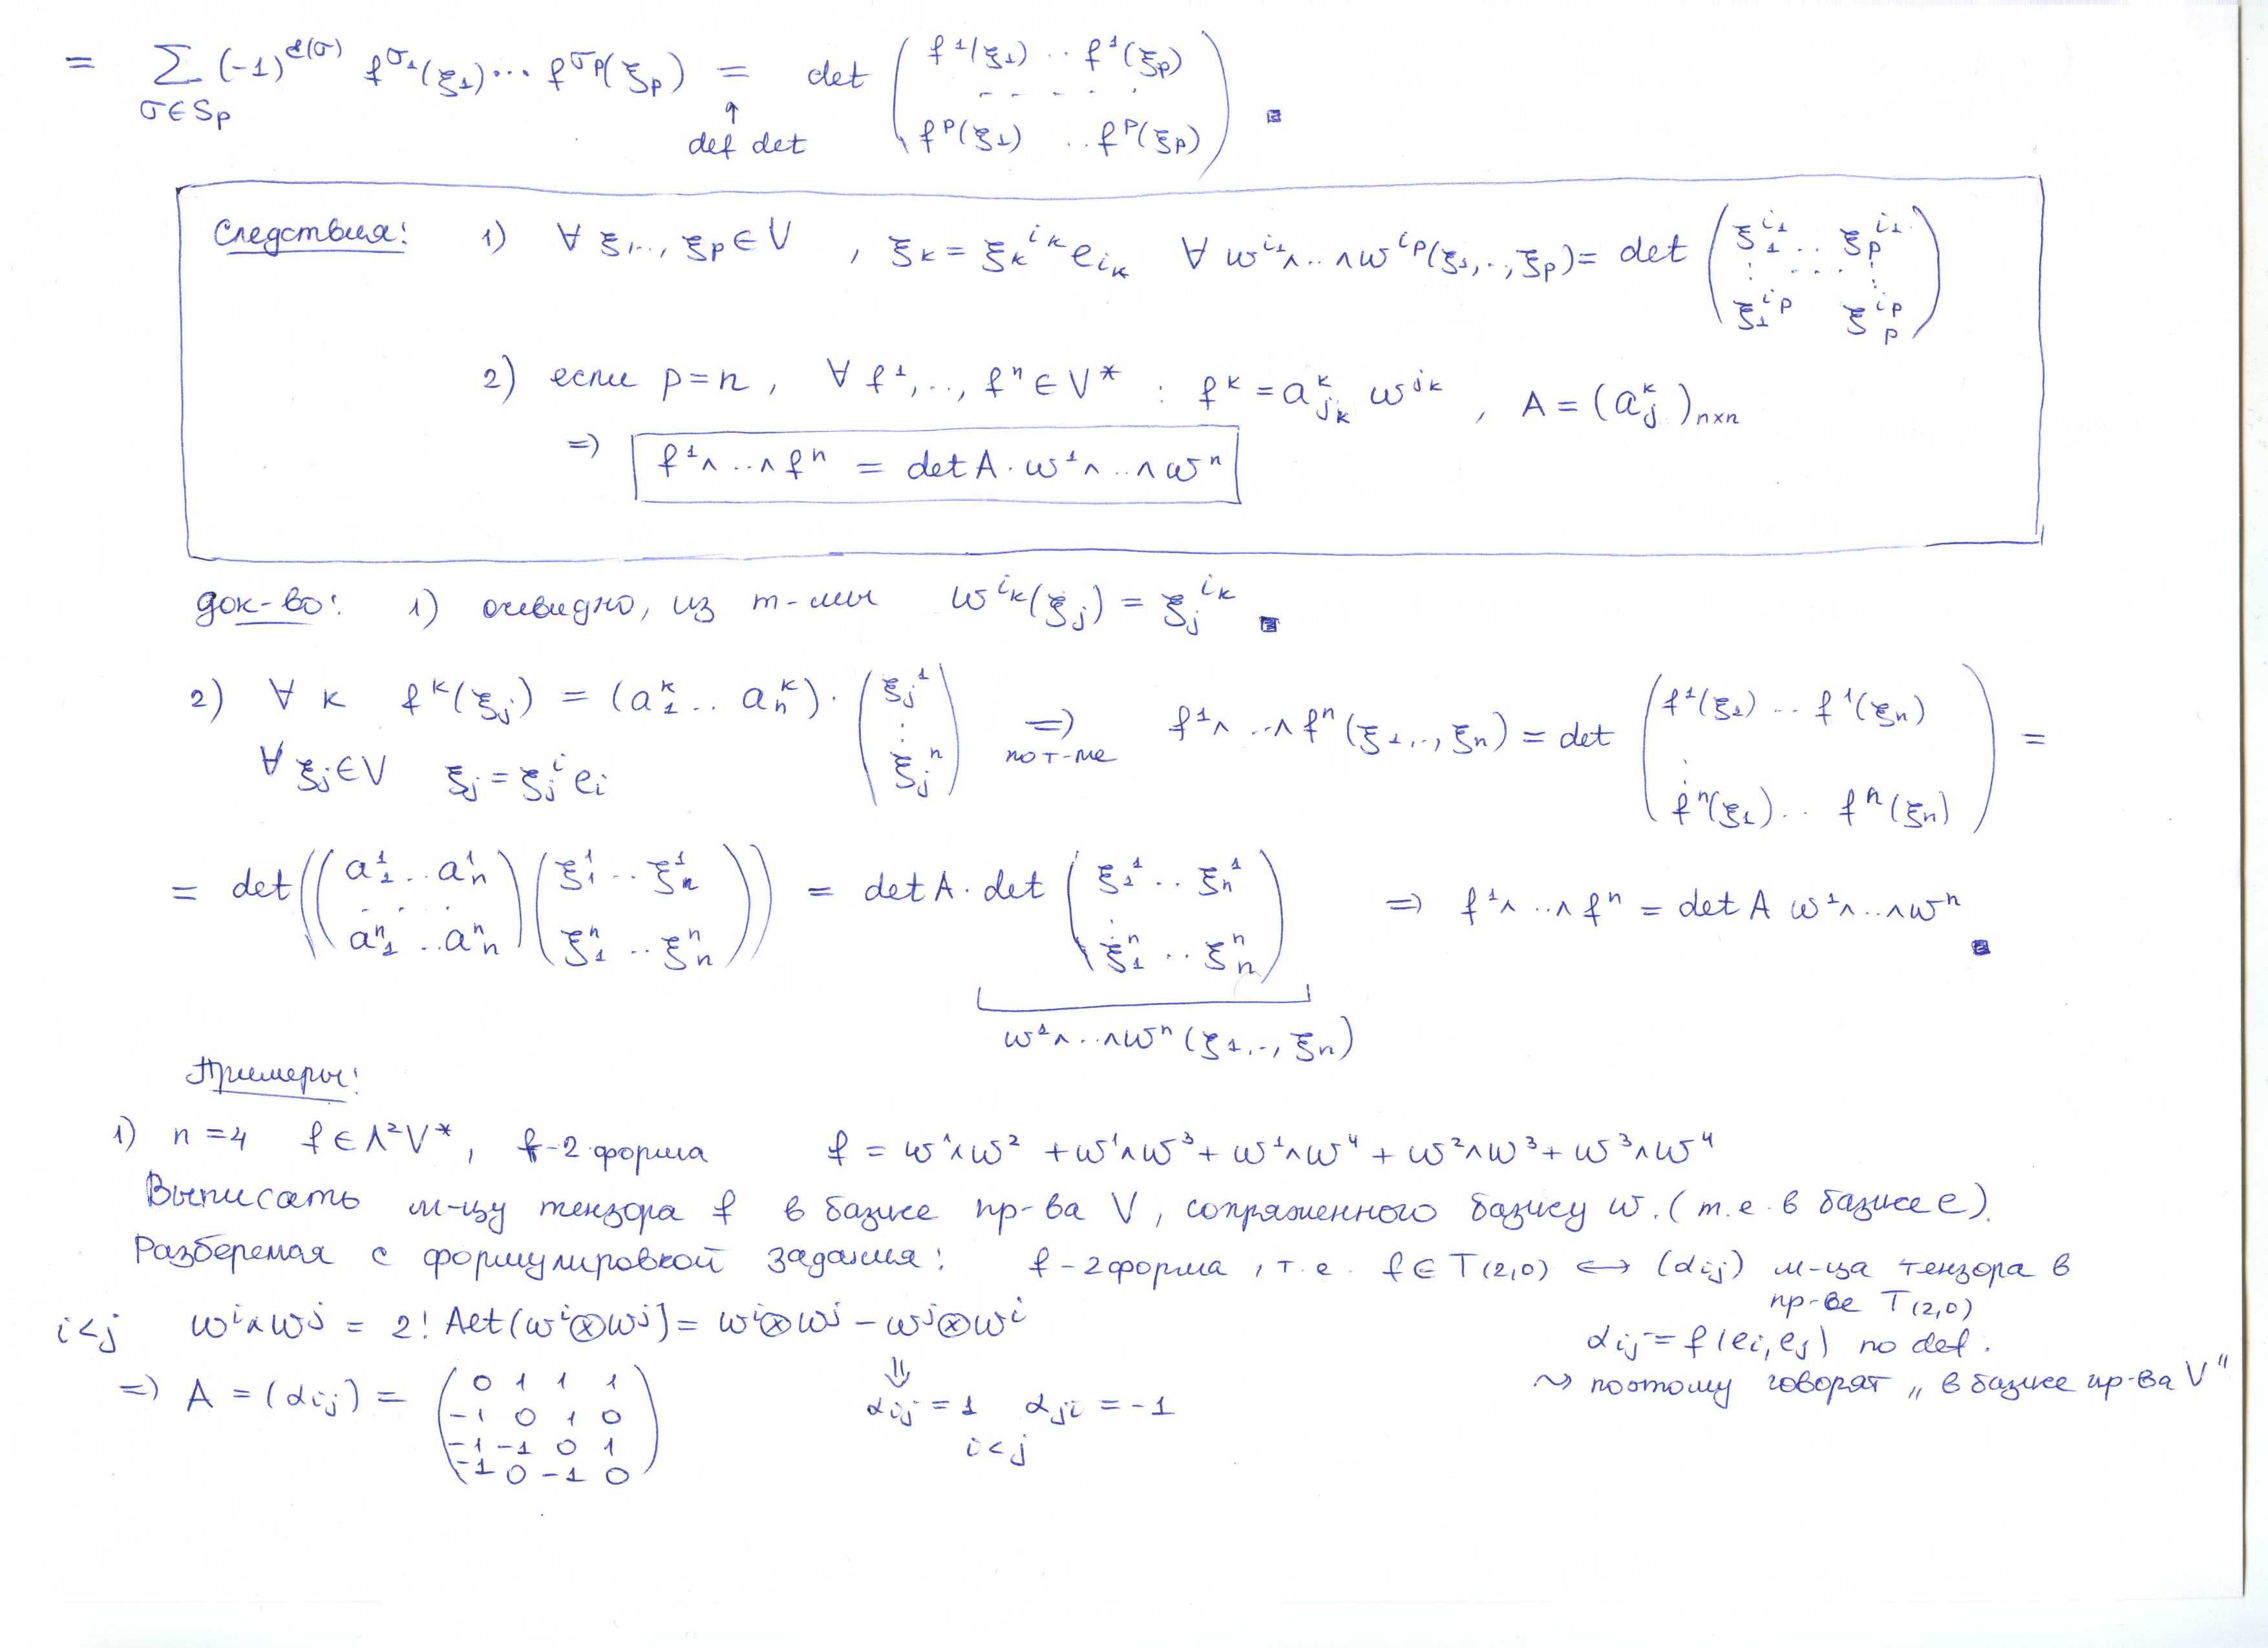
\includegraphics[height=0.49\textheight, width=\textwidth]{05007}
		\n
		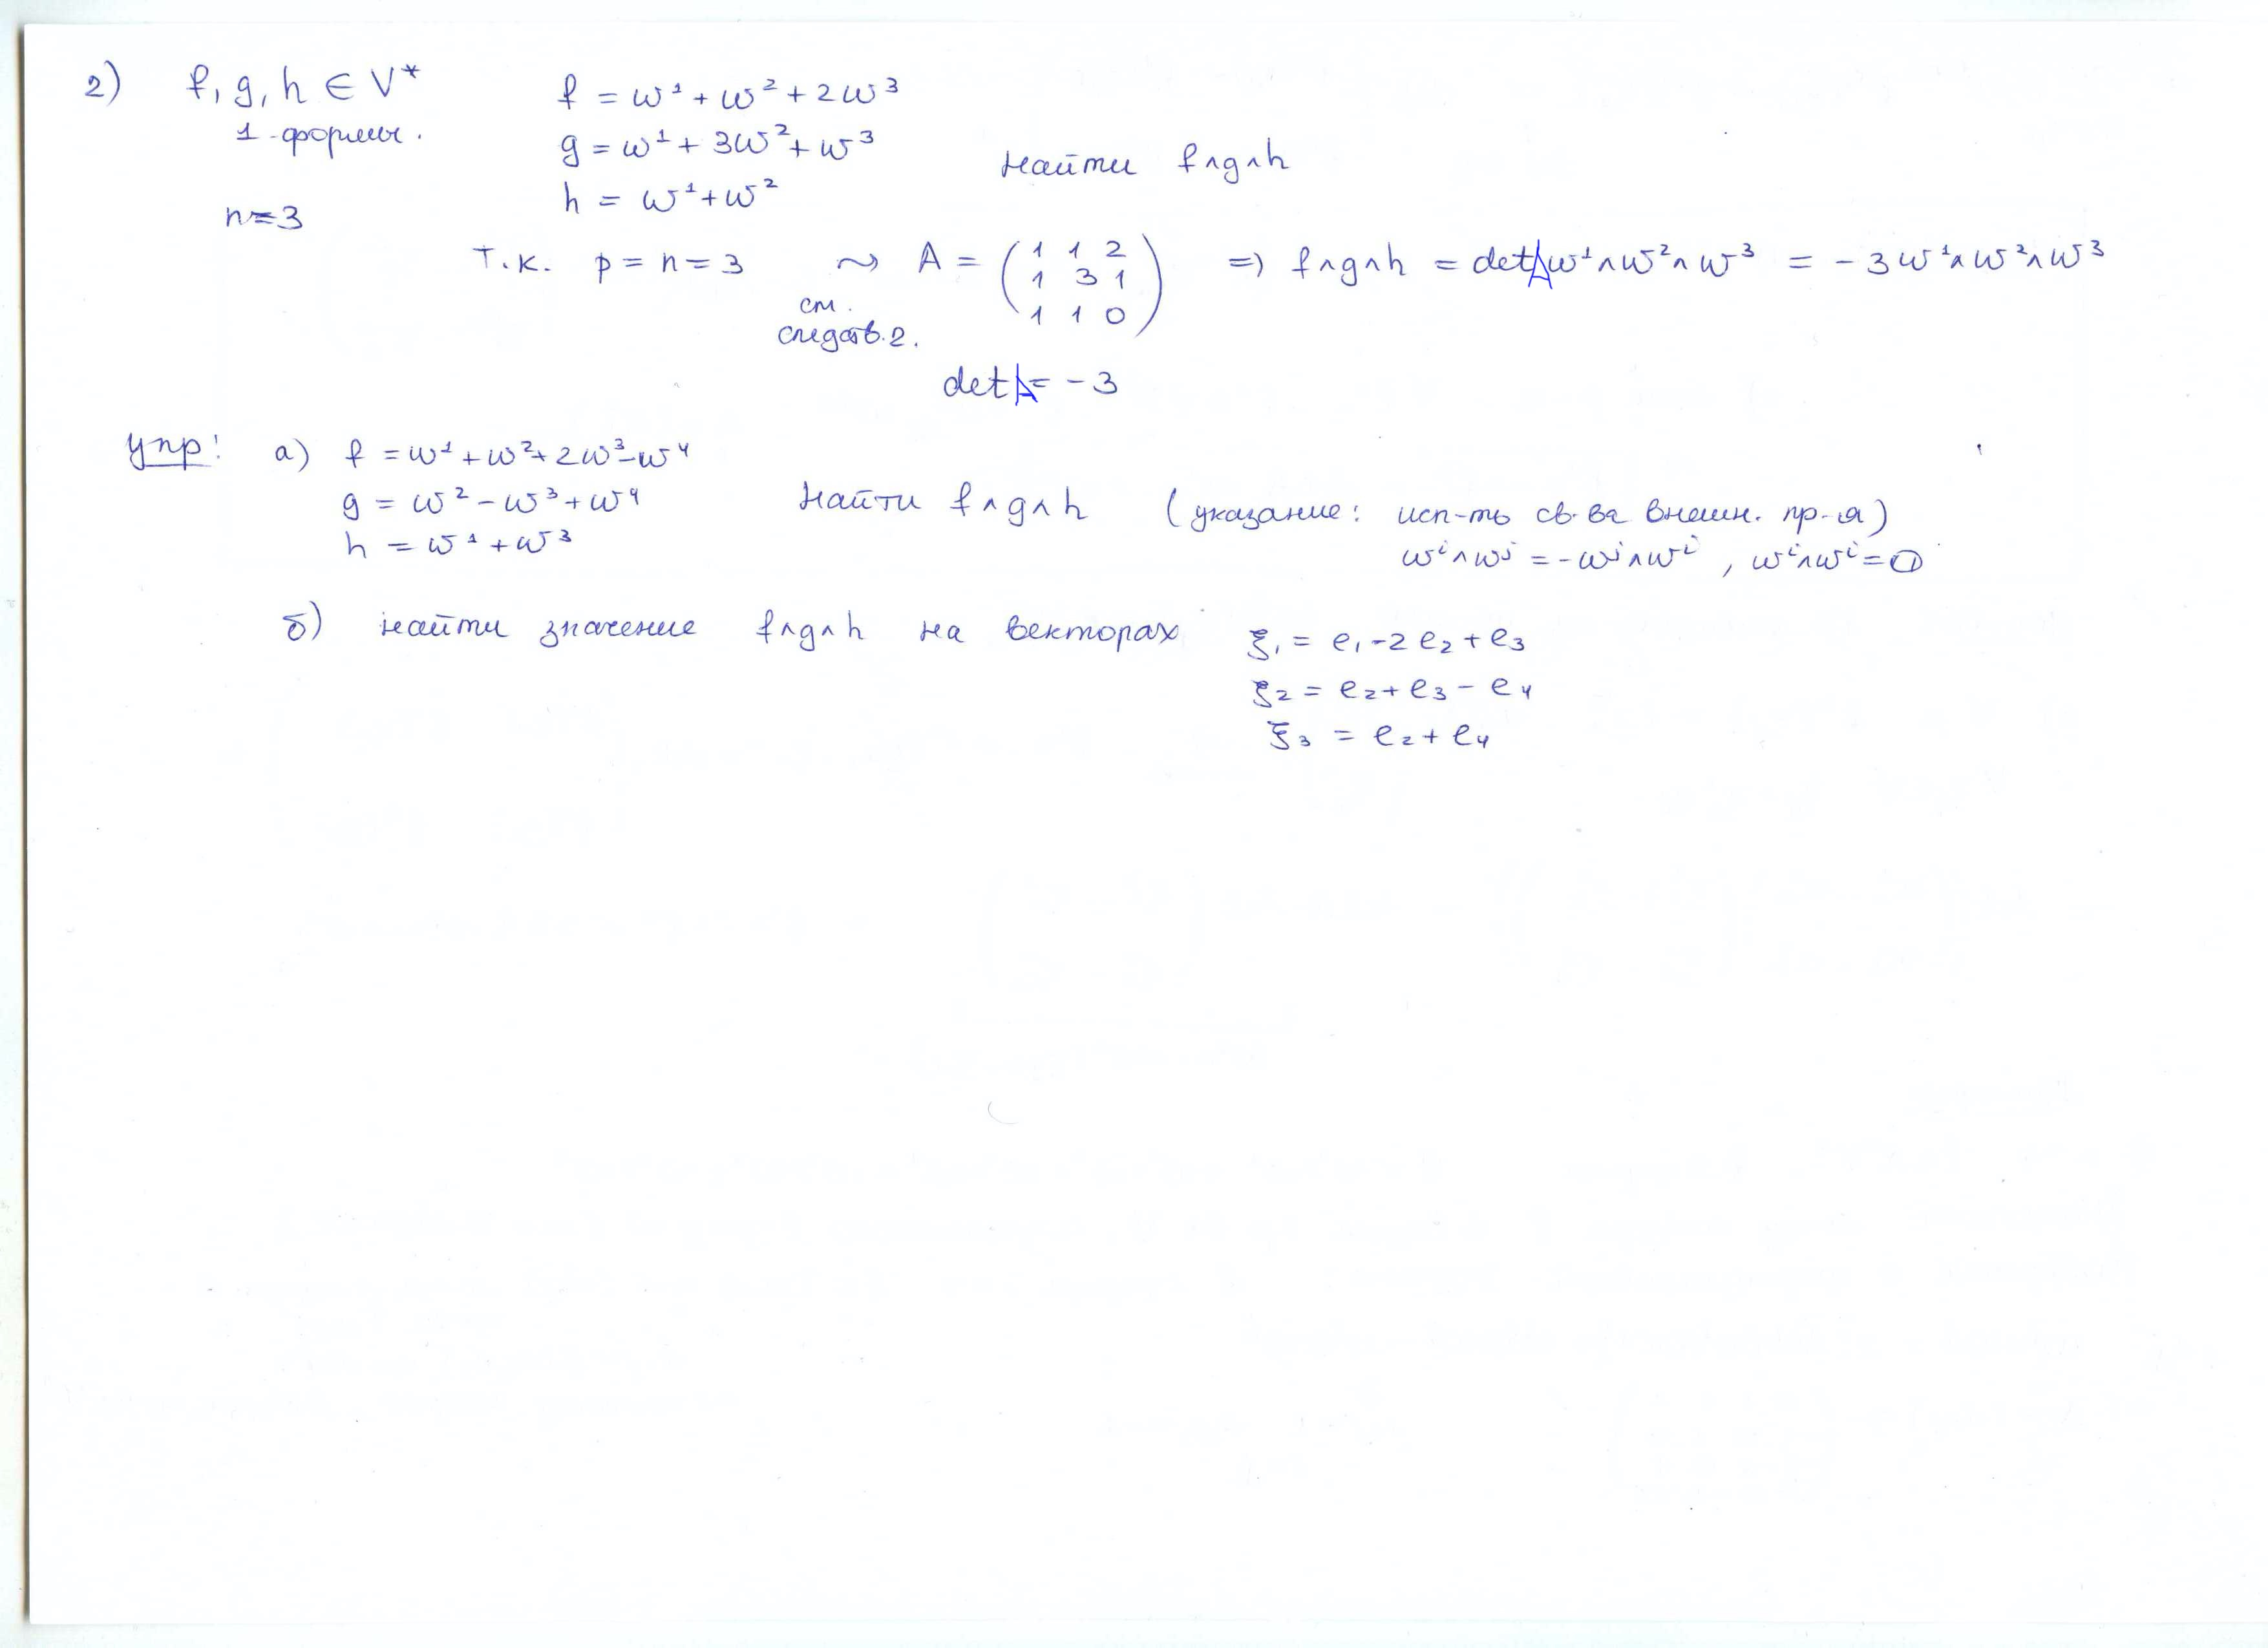
\includegraphics[height=0.49\textheight, width=\textwidth]{05008}
		\n
		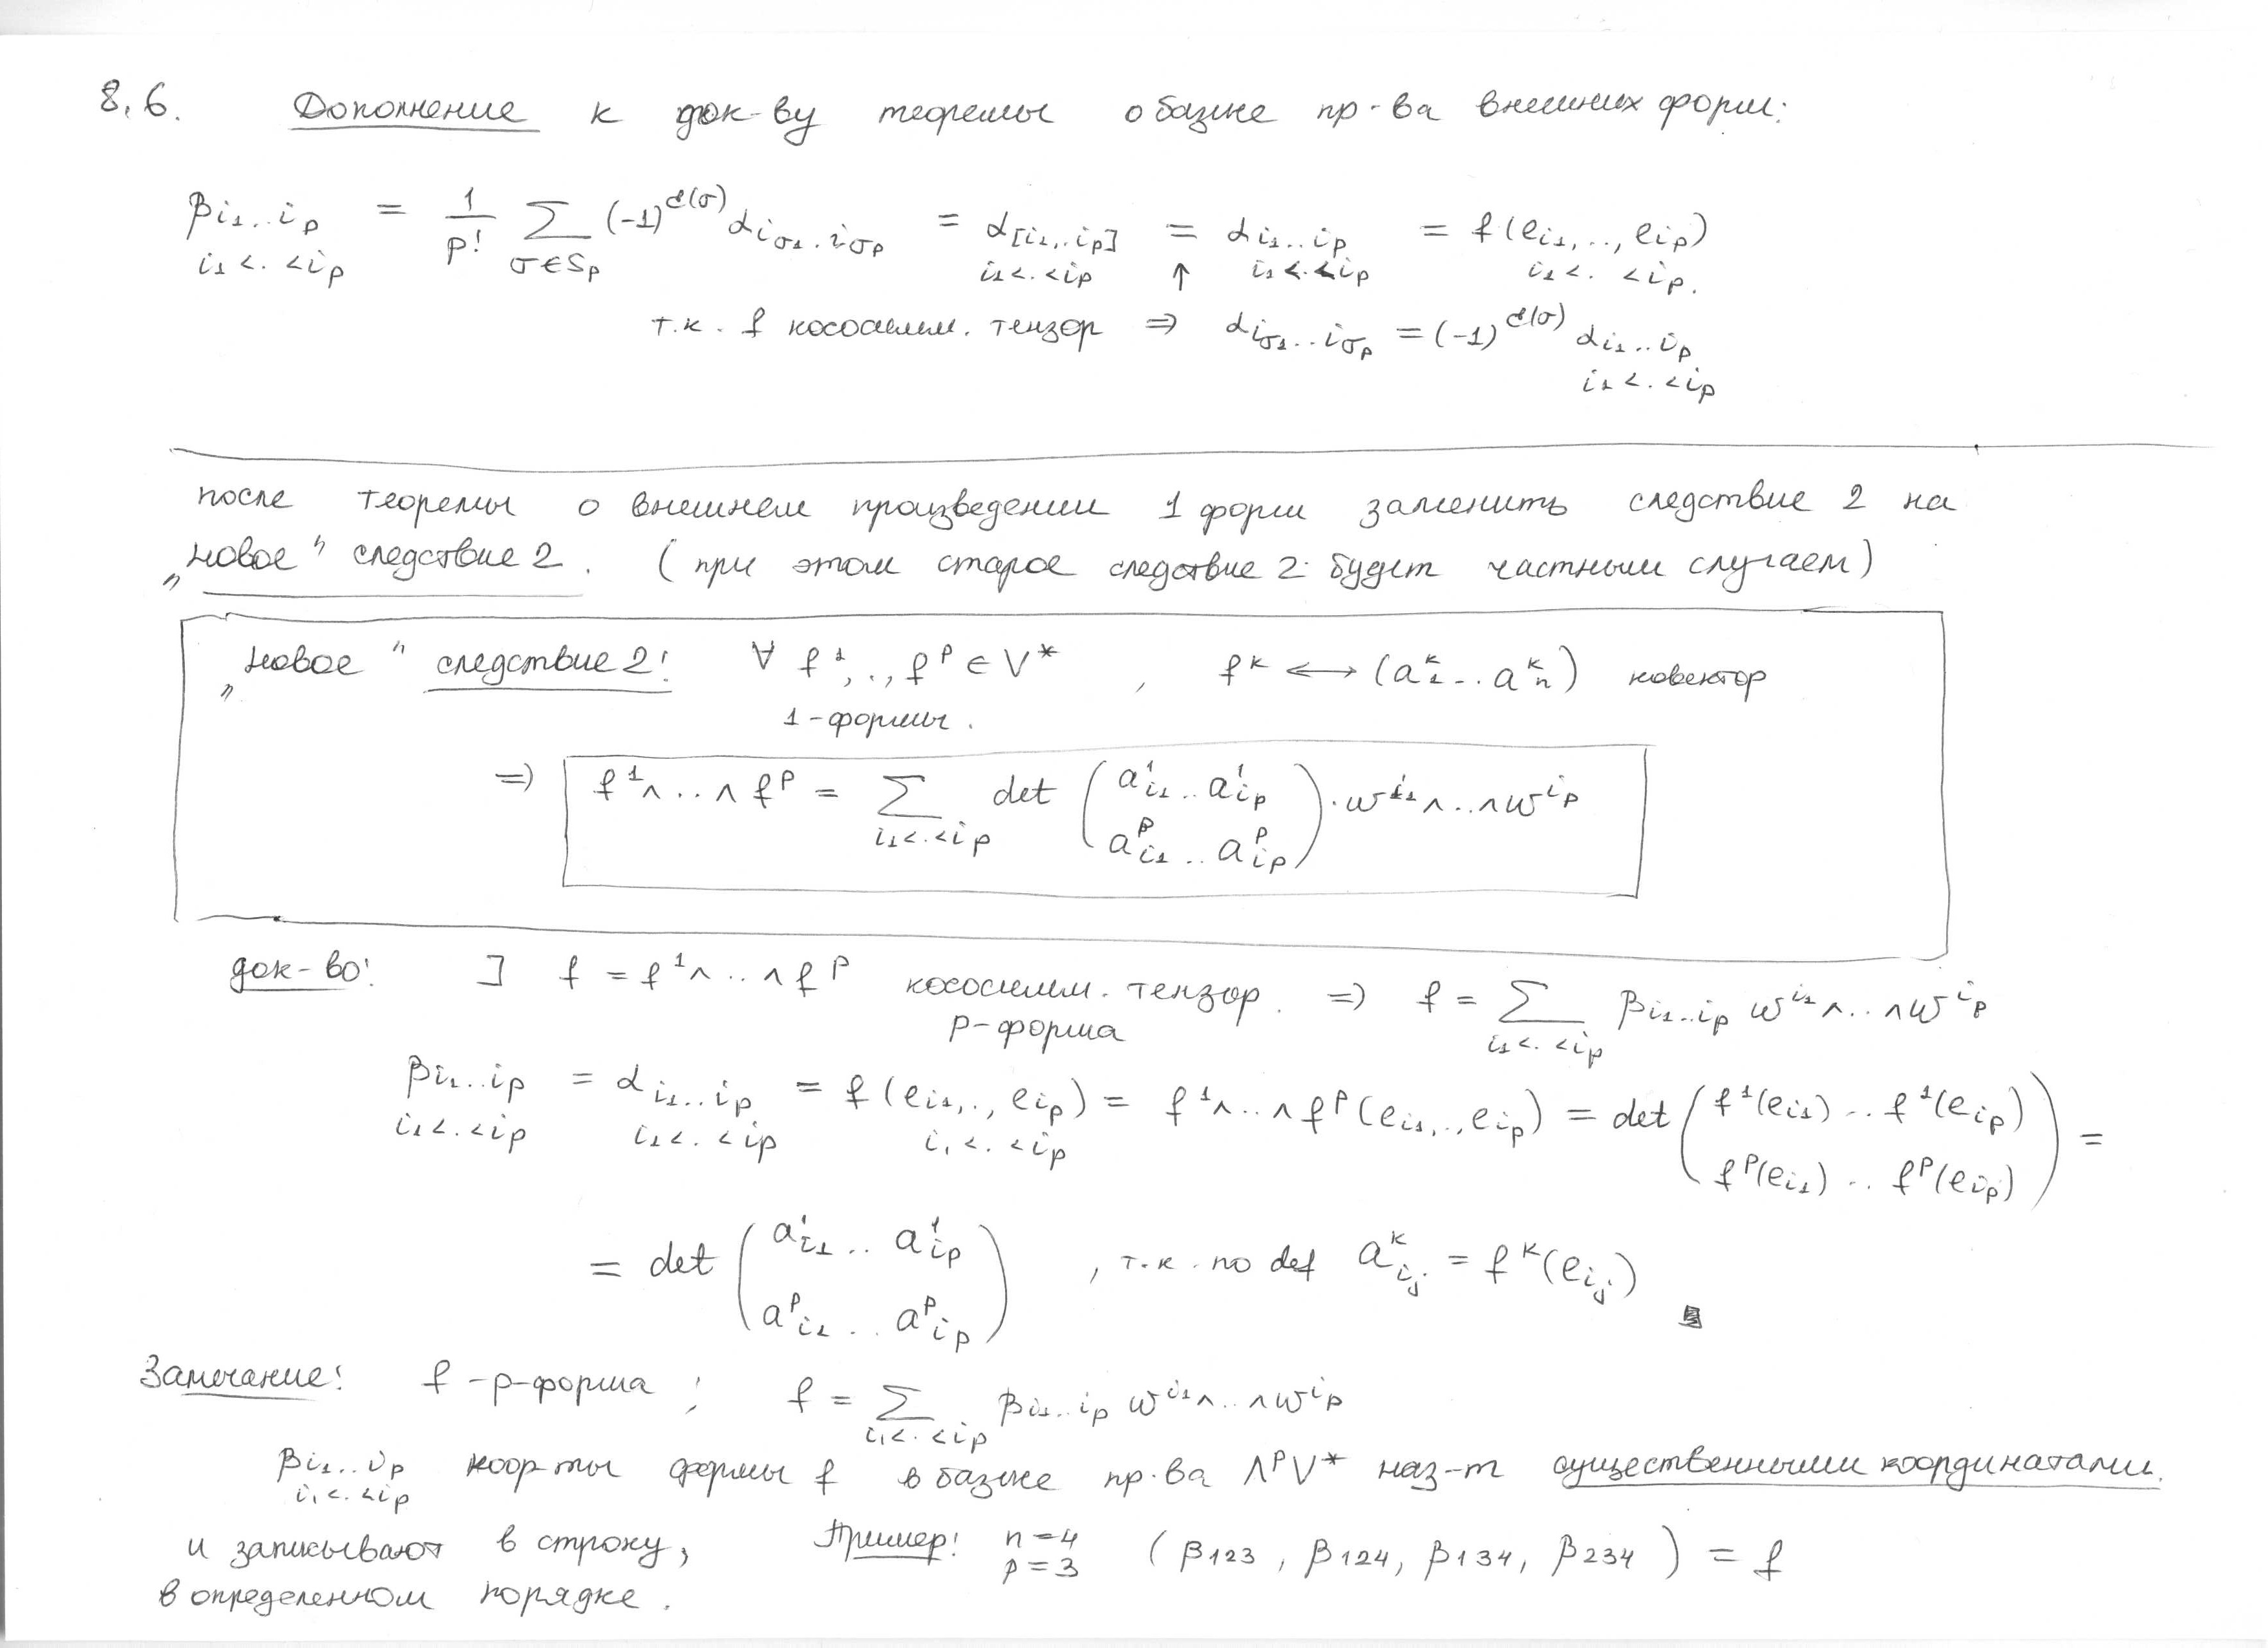
\includegraphics[height=0.49\textheight, width=\textwidth]{dopoln8_6}	
\end{document}